 vim: tw=80

\chapter{Measurement of the Triple-Differential Dijet Cross Section}
\label{sec:measurement}

The motivation for a triple-differential dijet cross section measurement which
optimally exploits the kinematics of the dijet system is given in
Chapter~\ref{sec:theory_predictions}. The theoretical considerations are completed
by providing a comprehensive measurement of these cross sections at the CMS
detector which allow detailed studies of the proton structure as discussed in
Chapter~\ref{sec:pdf_constraints}. 

Section~\ref{sec:datasets} discusses the
analyzed data samples, while the selection of dijet events meeting all quality
criteria are reviewed in Section~\ref{sec:event_selection}. A comparison with
simulated events and subsequently the correction of the measured data for
detector effects using an unfolding procedure is explained in detail in
Section~\ref{sec:simulated_events} and Section~\ref{sec:unfolding}. Uncertainty
Sources of experimental origin which affect the cross section measurement are

Finally, the comparison of unfolded data to NLO predictions is presented in
Section~\ref{sec:nlo_comparisons}. Comparisons to NLO calculations with matched
parton showers from the recently released Herwig~7 MC event generator are of
particular interest.

\section{Data samples}
\label{sec:datasets}

The measurement is based on a data sample collected by CMS in the 2012 run
period of the LHC at a center-of-mass energy of $\sqrt{s} = 8 \si{\TeV}$. The
accumulated data corresponds to a total integrated luminosity of $\mathcal{L} =
19.71 \si{\fbinv}$. 

The 2012 LHC run is divided into four periods A, B, C and D and the datasets are
split into samples according to the run period. Each dataset is further split up
into subsets containing only a fraction of the events triggered by a specific
group of triggers. The events triggered by a prescaled jet trigger were streamed
into the datasets \texttt{Jet} and \texttt{JetMon} while the events of the
unprescaled jet triggers are moved into the datasets \texttt{JetHT}. As this
assignment changed over the 2012 run period, great care has been taken to only
select the correct subset of events. The used datasets and the luminosity of
each dataset can be seen in Table~\ref{tab:data:datasets}.

\begin{table}[htbp]
    \centering
    \caption[Datasets of the 2012 LHC run period]
       {The complete 2012 data comprises 4 datasets collected in the run periods
           A, B, C and D. As the dataset names, in which the events selected by the
           jet triggers are stored, changed over time, great care has to be
           taken to select the correct subset of events from each dataset.}
    \label{tab:data:datasets}
    \begin{tabular}{llll}
    \toprule
    Run & Run Range & Dataset & Luminosity\\\midrule
    A & 190456--193621 & /Jet/Run2012A-22Jan2013-v1/AOD & \SI{0.88}{\fbinv}\\
    B & 193834--196531 & /Jet[Mon,HT]/Run2012B-22Jan2013-v1/AOD & \SI{4.49}{\fbinv}\\
    C & 198022--203742 & /Jet[Mon,HT]/Run2012C-22Jan2013-v1/AOD & \SI{7.06}{\fbinv}\\
    D & 203777--208686 & /Jet[Mon,HT]/Run2012C-22Jan2013-v1/AOD & \SI{7.37}{\fbinv}\\ 
    \bottomrule
    \end{tabular}
\end{table}

\subsection{Monte Carlo Samples}

To compare the data distributions with simulated events, two Monte-Carlo event
generators were considered. An overview about the Monte-Carlo generators is
given in Section~\ref{subsection:mc_generators}. Each MC generator is utilizing an
optimized tune to simulate the underlying event. Additionally the data samples
contain not only the hard interaction but also a model for pile-up collisions,
through which additional soft scattering events following the pile-up
distribution in data are mixed into the event.

The Madgraph+P6 Monte Carlo sample is generated with a multi-leg improved QCD
process. By using Madgraph, the LO matrix elements do not only contain the $2
\rightarrow 2$ matrix elements, but also the $2 \rightarrow 3$ matrix elements
which better describe multijet events, but have to be matched to subsequent
parton shower. The underlying event is modeled using the tune $Z2*$. The parton
shower and hadronization is carried out using the Pythia~6 event generator which
is interfaced to Madgraph by the LHE event record.

Furthermore a Pythia 8 data sample is analyzed. While including only the $2
\rightarrow 2$ LO matrix elements, the event simulation and the underlying event
tune are improved in this newer version of the Pythia Monte Carlo generator.

Both Monte-Carlo samples are processed through the complete CMS detector
simulation to allow studies of the detector response and compare to measured
data on detector level. 
\todo{add table with complete list, xs and events in appendix}
\begin{table}[htp]
    \centering
    \caption[Monte Carlo datasets]{The official MC production samples used in
    the analysis were generated as slices in the \pt or HT phasespace. A
    complete list of all subsamples and the corresponding sub-samples can be found
     in~\ref{mc_samples}.}
    \label{tab:montecarlo:datasets}
    \begin{tabular}{lc}
    \toprule
    Dataset Name & Dataset Identifier\\\midrule
    Madgraph & \makecell[l]{/QCD\_HT-XXToXX\_TuneZ2star\_8TeV-madgraph-pythia/\\
        \phantom{aaaa}Summer12\_DR53X-PU\_S10\_START53\_V7A-v1/AODSIM}\\
        Pythia 8 & \makecell[l]{/QCD\_Pt-XXtoXX\_Tune4C\_8TeV\_pythia8/\\
        \phantom{aaaa}Summer12\_DR53X-PU\_S10\_START53\_V7A-v1/AODSIM}\\
    \bottomrule
    \end{tabular}
\end{table}

Since jet cross sections which are measured as a function of the transverse
momentum fall steeply with increasing \pt, it is not possible to generate a
large number of high-\pt events in a reasonable time. Therefore the event
generation is split into different phase space region binned in HT, the scalar
sum of the transverse momentum of all jets, or the leading jet \pt. The
different phase space regions are then stitched together later in the data
analyses while taking into account the cross section in the different phase
space regions.  Table~\ref{tab:montecarlo:datasets} gives the employed Monte
Carlo datasets.

\section{Event selection}
\label{sec:event_selection}

The selection of dijet events is based on several quality criteria recommended by CMS
for jet analyses. Furthermore phase spaces cuts ensure the applicability and
comparison of NLO theory calculations.

\subsection{Certified Data Selection}

The first step in the event processing chain is to only pick data from runs and
luminosity sections (LS) which fullfill certain criteria. These include the
proper performance of all detector subsystem and the succesful passing of the
data quality monitoring (DQM) steps during the validation process. The good
lumisections within a run are announced using a JSON data file, called
\textit{Golden JSON}. The applied lumisection certification
file\footnote{\texttt{Cert\_190456-208686\_8TeV\_22Jan2013ReReco\_Collisions12\_JSON}}
in our analysis is based on the final event reconstruction of the 2012 datasets.

\subsection{Trigger Selection}

To measure and reconstruct the \ptavg spectrum of the dijet production, a set of
single jet triggers have been used. Single jet triggers consist of one L1
trigger seed and multiple HLT filters. The L1 trigger has a smaller threshold to
ensure full efficiency versus \pt for the HLT trigger. Table~\ref{tab:triggers}
shows the full set of single jet triggers employed. Since the \pt spectrum is
exponentially falling and the rates for low-\pt jets are very high, it is not
possible to use a single unprescaled trigger to select all interesting events.
Therefore a set of prescaled low-\pt triggers each with different prescales is
used to collect sufficient data in the lower part of the \pt spectrum.
Additionally one unprescaled trigger is used in the region where the jet rate is
sufficiently small to collect all events. The prescales are taken into account
again when the spectrum is reconstructed. 

\begin{table}[htbp]
    \centering
    \caption[Single Jet Trigger Paths]{Used trigger paths in the analysis. Each path is used in an mutually exclusive phase space in \ptavg. The
            $p_{\mathrm{T},.99\%}$ threshold gives the value at which a trigger reaches 99\% efficiency compared to lower
            reference trigger.}
    \label{tab:triggers}

    \begin{tabular}{lcccr}
        \toprule
        Trigger path  & L1 (\si{\GeV}) & HLT (\si{\GeV}) & $p_{\mathrm{T},.99\%}$ (\si{\GeV}) & Eff. Lumi \\\midrule
        HLT\_PFJet40  & 16                  & 40                   & --                     & 0.08 \si{\pbinv}\\
        HLT\_PFJet80  & 36                  & 80                   & 123                    & 2.12 \si{\pbinv}\\
        HLT\_PFJet140 & 68                  & 140                  & 192                    & 55.67 \si{\pbinv}\\
        HLT\_PFJet200 & 92                  & 200                  & 263                    & 0.26 \si{\si{\fbinv}}\\
        HLT\_PFJet260 & 128                 & 260                  & 353                    & 1.06 \si{\si{\fbinv}}\\
        HLT\_PFJet320 & 128                 & 320                  & 412                    & 19.71 \si{\si{\fbinv}}\\
        \bottomrule
    \end{tabular}
\end{table}


\begin{figure}[htbp]
    \centering
    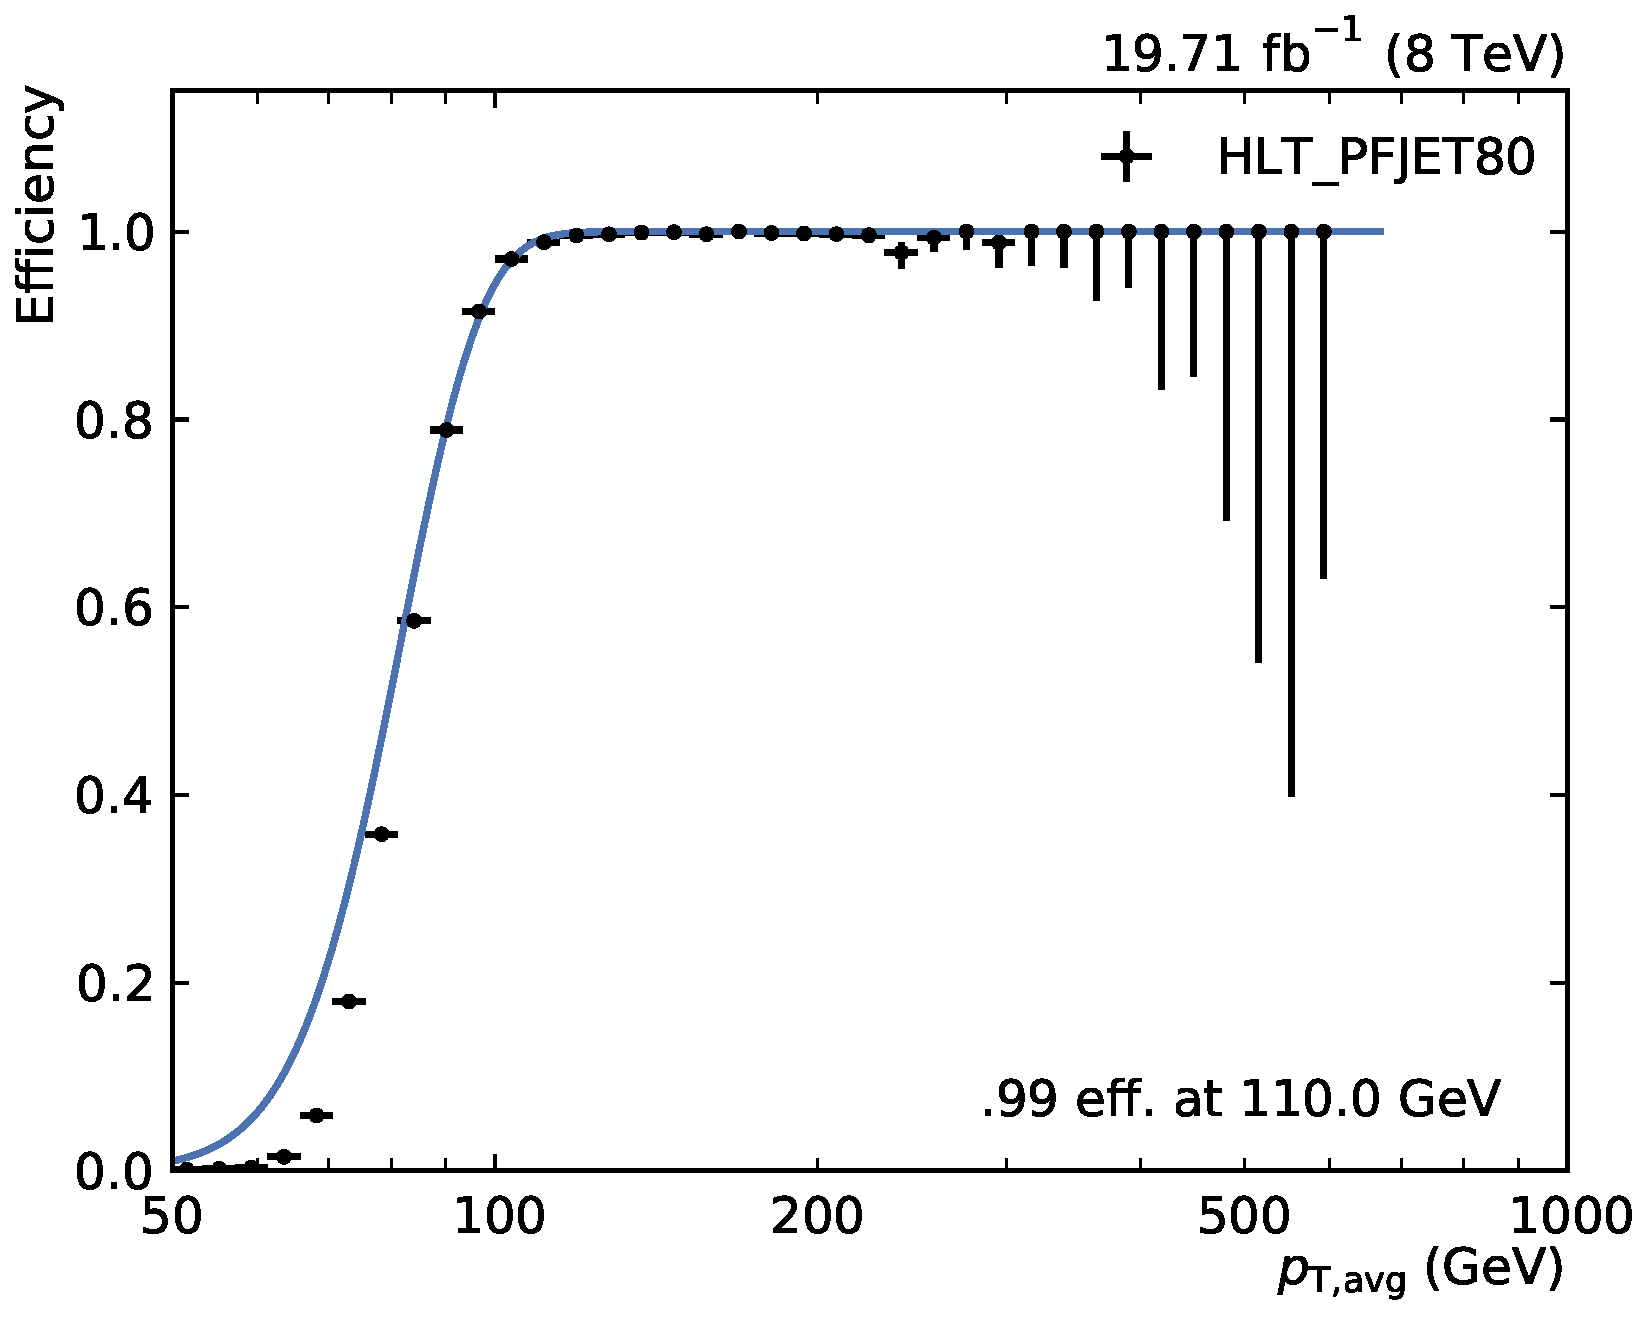
\includegraphics[width=0.45\textwidth]{figures/measurement/trigger_eff_HLT_PFJET80_default.pdf}\hfill
    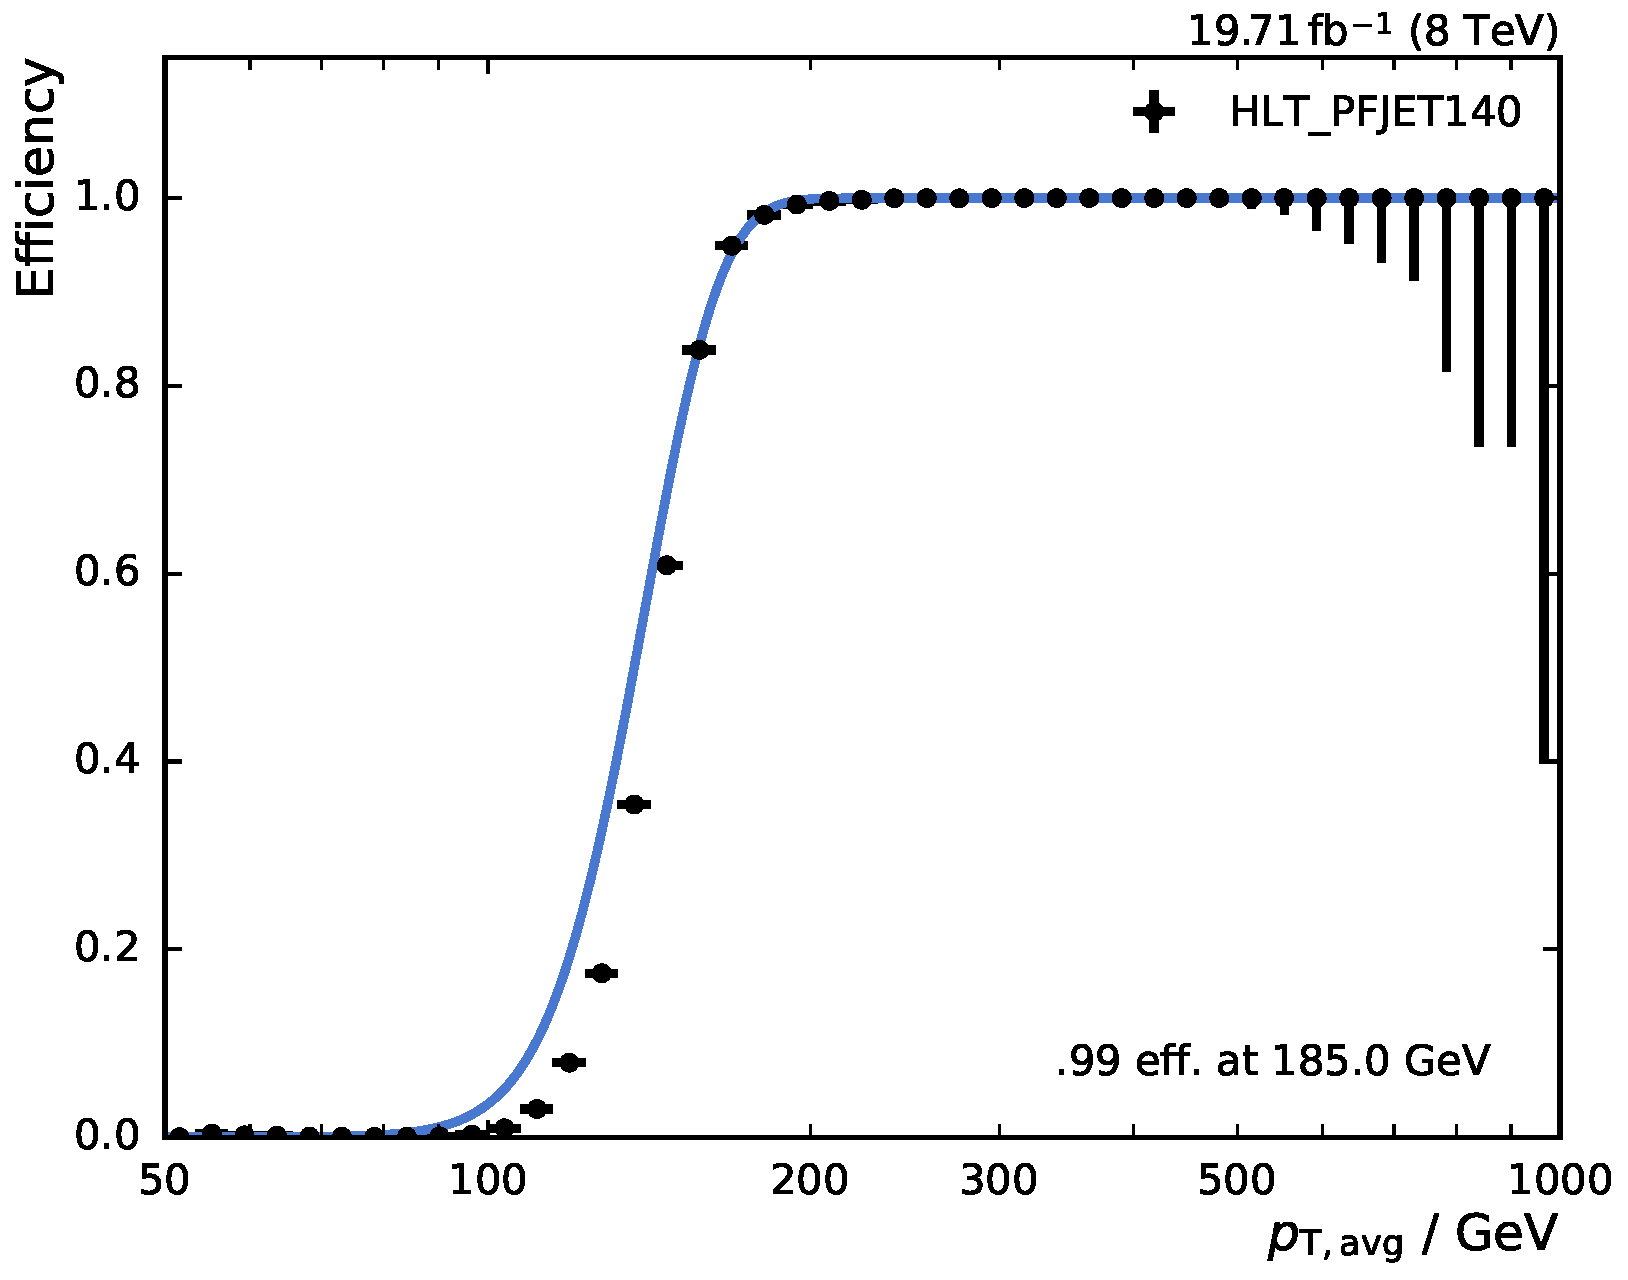
\includegraphics[width=0.45\textwidth]{figures/measurement/trigger_eff_HLT_PFJET140_default.pdf}
    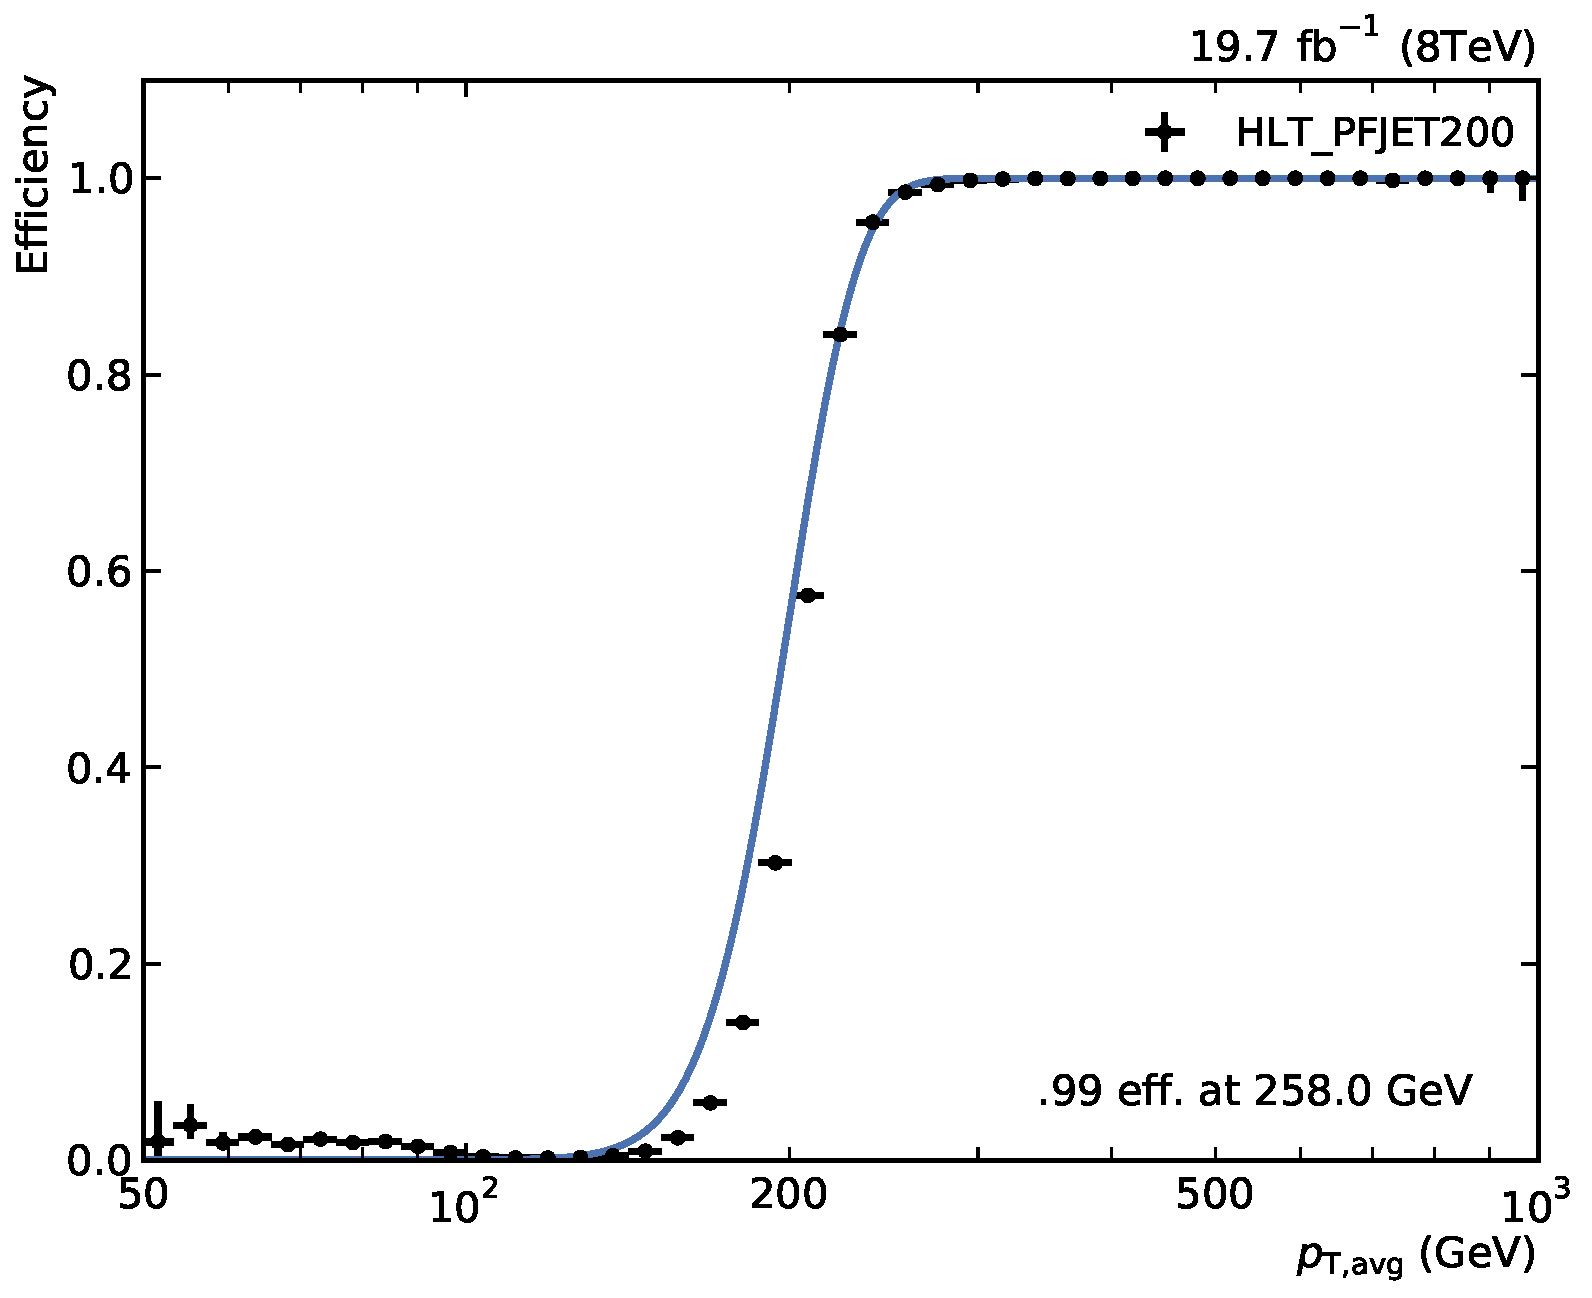
\includegraphics[width=0.45\textwidth]{figures/measurement/trigger_eff_HLT_PFJET200_default.pdf}\hfill
    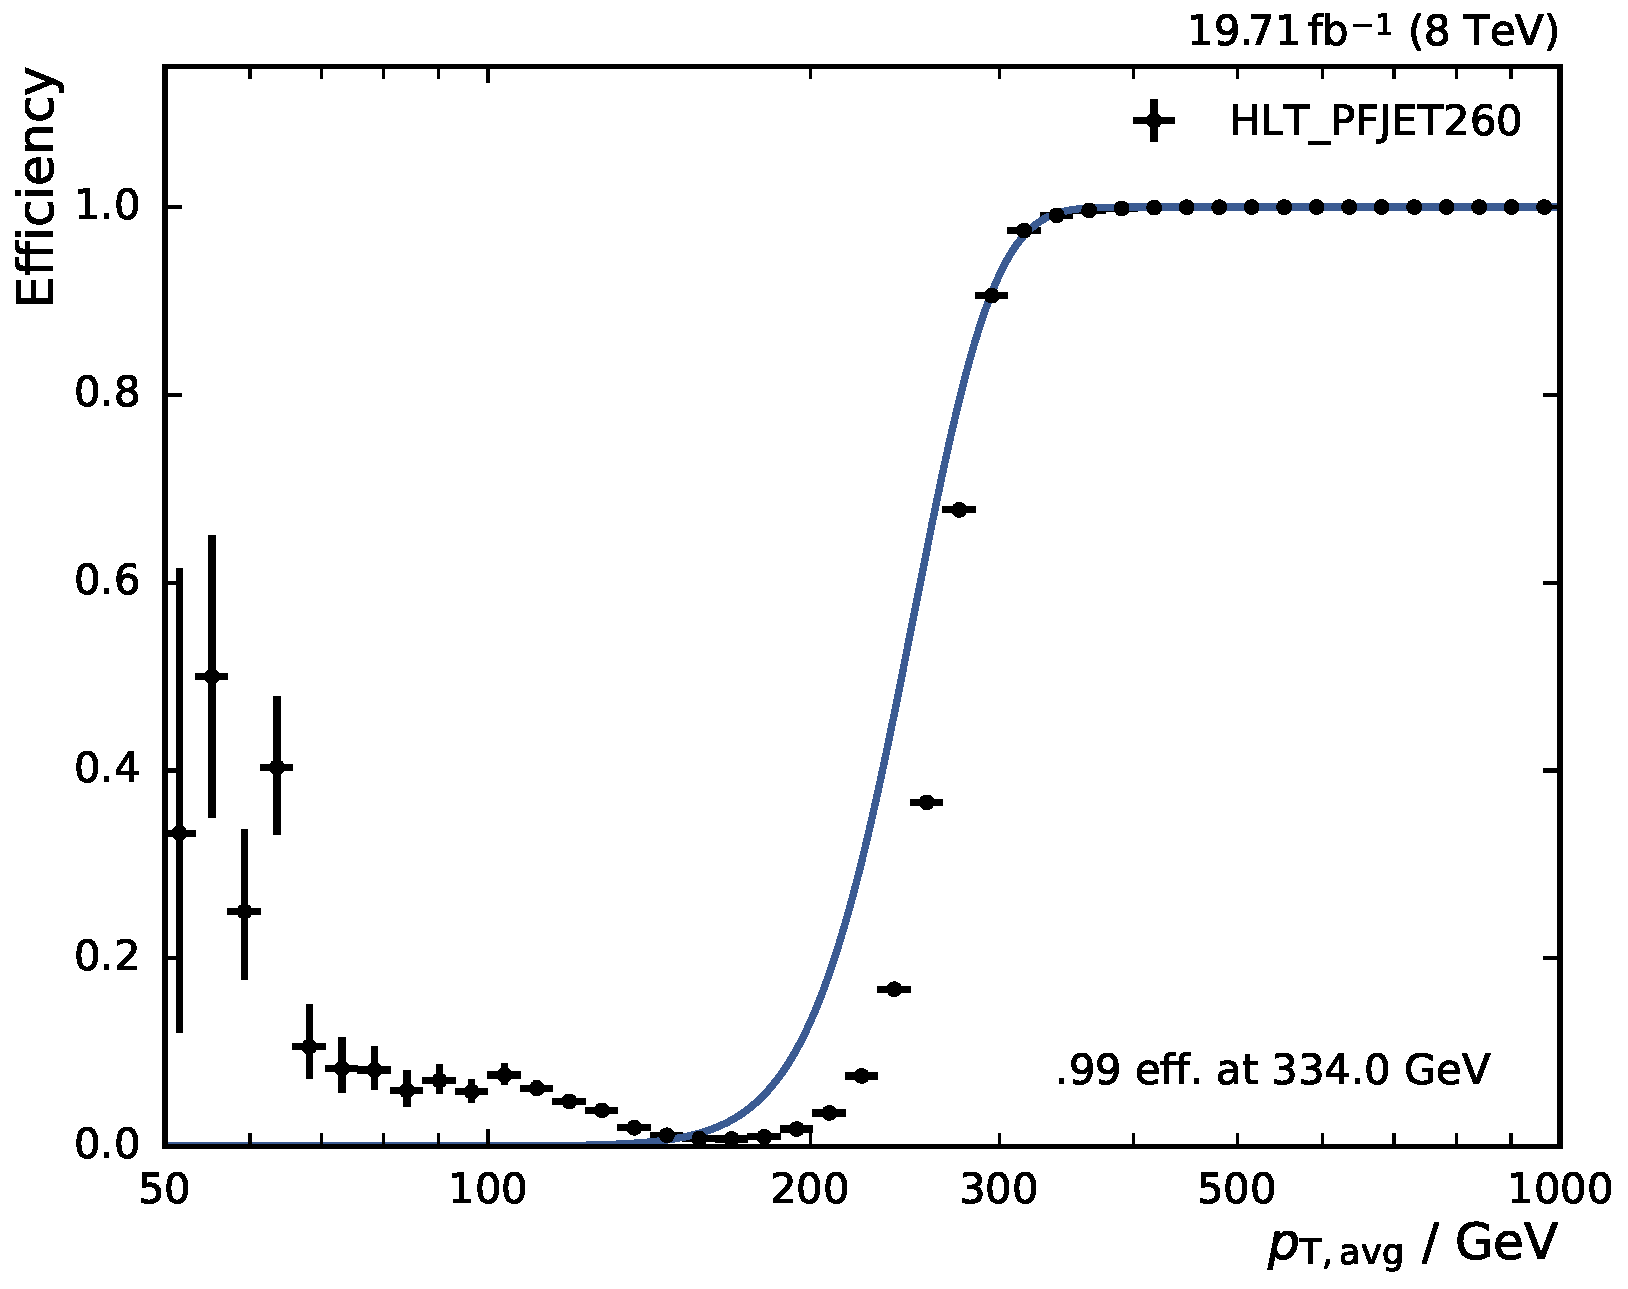
\includegraphics[width=0.45\textwidth]{figures/measurement/trigger_eff_HLT_PFJET260_default.pdf}
    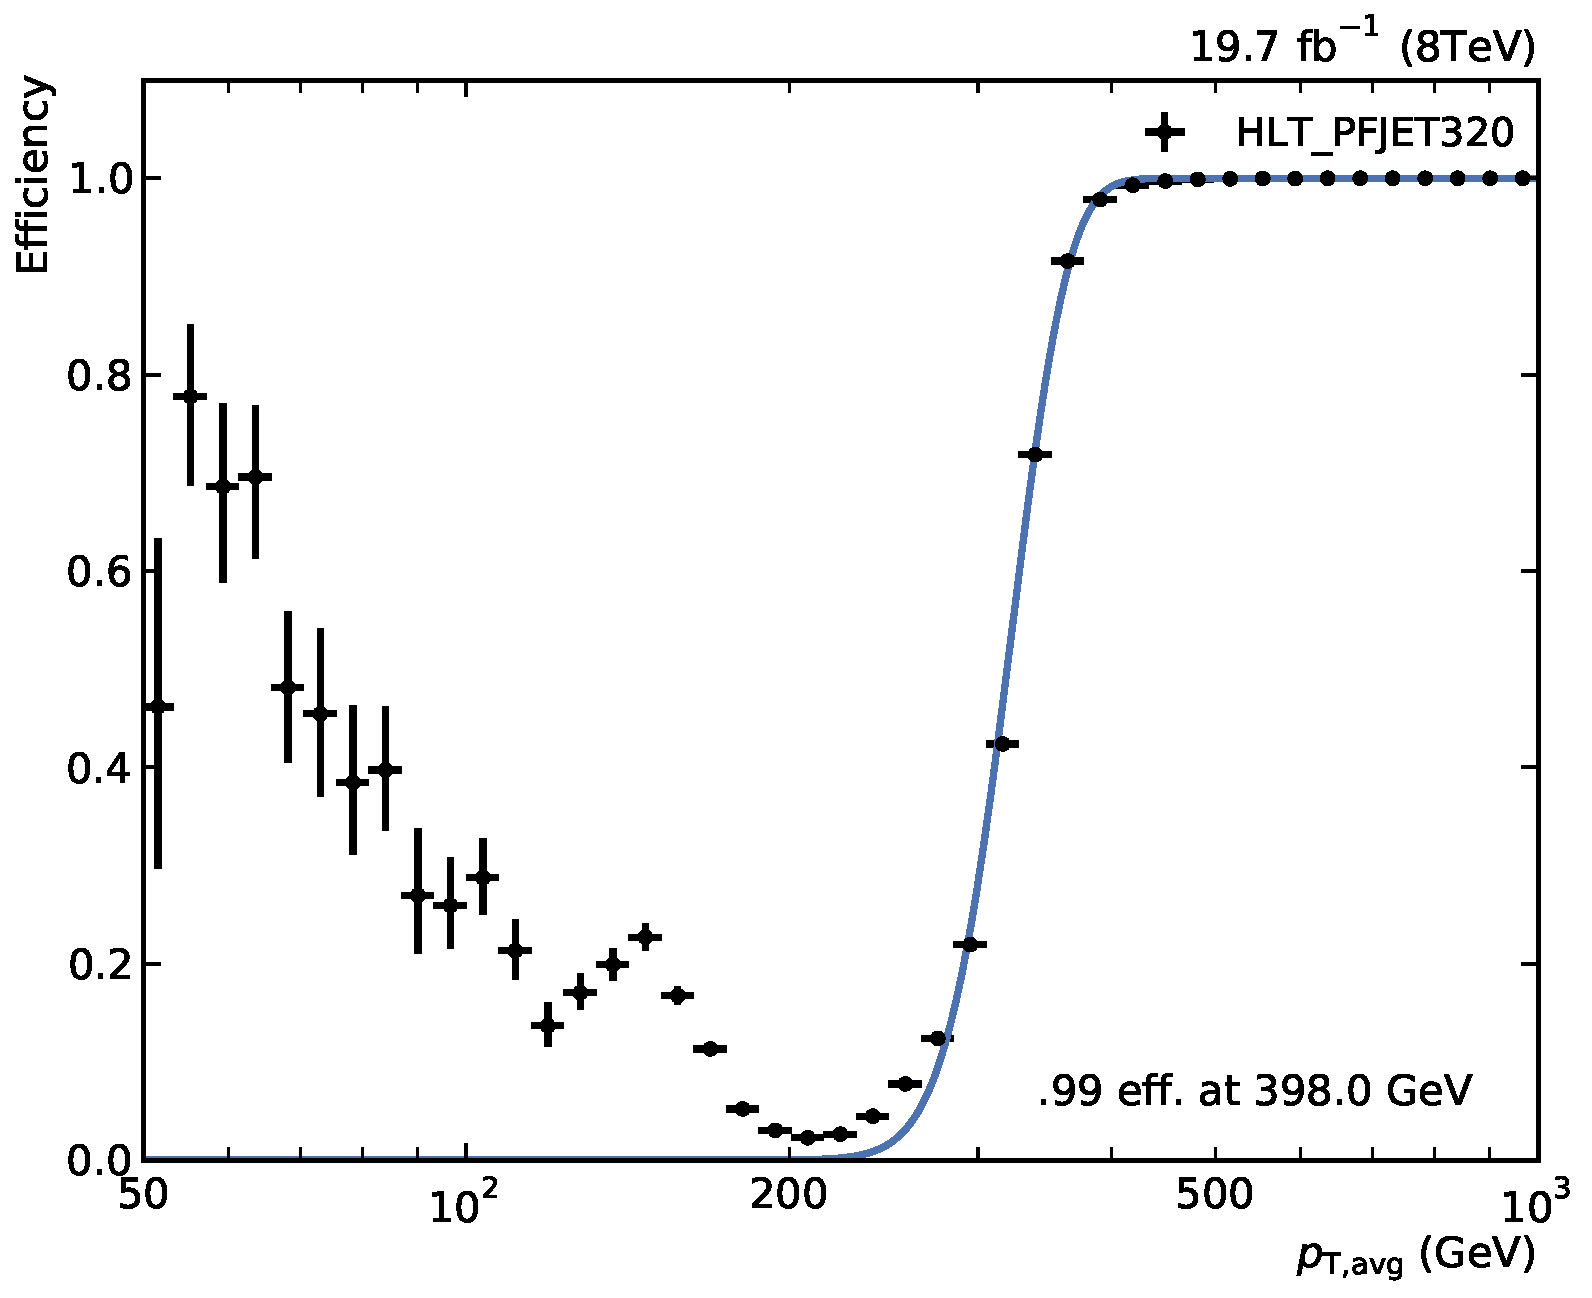
\includegraphics[width=0.45\textwidth]{figures/measurement/trigger_eff_HLT_PFJET320_default.pdf}\hfill
    \caption[Turn-on curves of single jet HLT trigger paths]{Trigger efficiencies turn-on curves for the single jet trigger
    paths used in the analysis. To determine the 99\% efficiency threshold, the
    trigger paths are fitted using a sigmoid function taking into account the
    uncertainties using Clopper-Pearson confidence intervals.}
    \label{fig:trigger_eff}
\end{figure}

The reconstruction algorithms and the jet energy corrections applied on HLT
level are slightly different compared to the final data reconstruction.
Additionally the trigger efficiency is not calculated versus $\ptjet$ which was
used in the trigger decision, but versus the \ptavg of the dijet system used in
this analyses. Therefore the trigger paths show a turn-on behaviour as can been seen in
Figure~\ref{fig:trigger_eff} and it is neccessary to determine the threshold at
which a trigger is fully efficient.

Due to the different prescales introduced by each trigger path, it is not
trivially possible to calculate the efficiency by dividing the number of passed events for
one trigger by dividing through the number of events passed by the previous
trigger with the lower \pt threshold which is by definition fully efficient for
the higher trigger path. While it is possible to normalize the yield by the
effective luminosity seen by each trigger, this introduces statistical
fluctuations due to the large differences of the number of events seen by each
trigger caused by the prescale factors.

When the L1 trigger and HLT trigger are processed, the objects passing the
trigger are stored. Therefore it is possible to re-emulate the trigger decision
by comparing the L1 jet \pt with the L1 trigger threshold and the HLT jet \pt
with the HLT threshold~\cite{Stober:2012abc}.

Similarly the trigger decision of the next higher jet trigger can be emulated
starting from the lower trigger path. A set of events $S_1 = \left\{E_i | T_A
(E_i) = true \right\}$ which was accepted  by the lower trigger path $T_A$ is
used to determine the subset $S_2 = \left\{E_i|T_A(E_i) \wedge  T_B(E_i)
\right\}$ which would also pass the higher trigger $T_B$. The ratio of both
event sets can be used to determine the efficiency as shown for each trigger
path in Figure~\ref{fig:trigger_eff} using the Equation~\ref{eq:trigger_eff}.
The error bars of the trigger efficiency are given by Clopper-Pearson confidence
intervals.

\begin{equation}
\label{eq:trigger_eff}
    f_{\mathrm{eff}} (x) = \frac{N(\left\{E_i|T_A(E_i) \wedge T_B(E_i), x)\right\}}{N(\left\{ E_i | T_A(E_i) = \mathrm{true} \right\} , x)}
\end{equation}

The efficiency versus \ptavg is fitted using the sigmoid function~\ref{eq:trigger_eff_fit} describing
the turn-on behaviour of the trigger paths. Each trigger was used in a region in which the efficiency
is larger than $99\%$. The actual used trigger efficiency deviate slightly from the once shown in Table~\ref{tab:triggers}
since the used trigger eff. thresholds were measured for each \ystar and \yboost bin and the most
conservative value was used.

\begin{equation}
\label{eq:trigger_eff_fit}
    f_{\mathrm{fit}} (x) = \frac{1}{2} \left( 1 + \erf \left(\frac{x-\mu}{\sqrt{2}\sigma}\right)\right)
\end{equation}

Table~\ref{tab:triggers} contains the L1 and HLT thresholds of each trigger and
the \ptavg value at which each trigger reaches 99\% efficiency.

It has to be mentioned, that there are also HLT trigger available which
specifically trigger on the average transverse momentum of the dijet system.
Naturally they appear to be the better choice for this analysis. The \ptavg
trigger paths were studied, but the performance is only comparable and partially
even slightly worse due to larger prescales applied to these trigger paths.

\subsection{Primary Vertex Selection}

The cuts on the primary vertex further reject beam background and off-centre bunch
crossings. Each event has to contain at least one primary vertex (PV) which is well
reconstructed within a distance of $|z_\mathrm{PV}| < \SI{24}{\centi \meter}$ to
the nominan interaction point of the detector. Futher more the radial distance
$\rho_\mathrm{PV}$ has to fullfill $\rho_\mathrm{PV} < \SI{2}{\centi\meter}$. To
ensure a high quality of the vertex reconstruction in the fit, the number of
degrees of freedom in the vertex fit $n_{\mathrm{dof,PV}}$ needs to be at least
four. This basically means that at least four tracks need to be present to
perform the vertex fit.

\subsection{Missing transverse energy cut}
\todo{cite jet met filter twiki}
If all particles could be identified and perfectly measured, the sum of the
transverse momenta would sum up to zero. The imbalance in the transverse
momentum of all visible particles, which can be measured in the detector, is
called the missing transverse momentum (MET). Neutrinos, for example, leave the
detector undetected and do contribute to the MET. MET is an important ingredient
in many measurements involving W bosons, top quarks or searches for physics
beyond the standard model which involve undetectable particles. 

\begin{figure}[htbp]
    \centering
    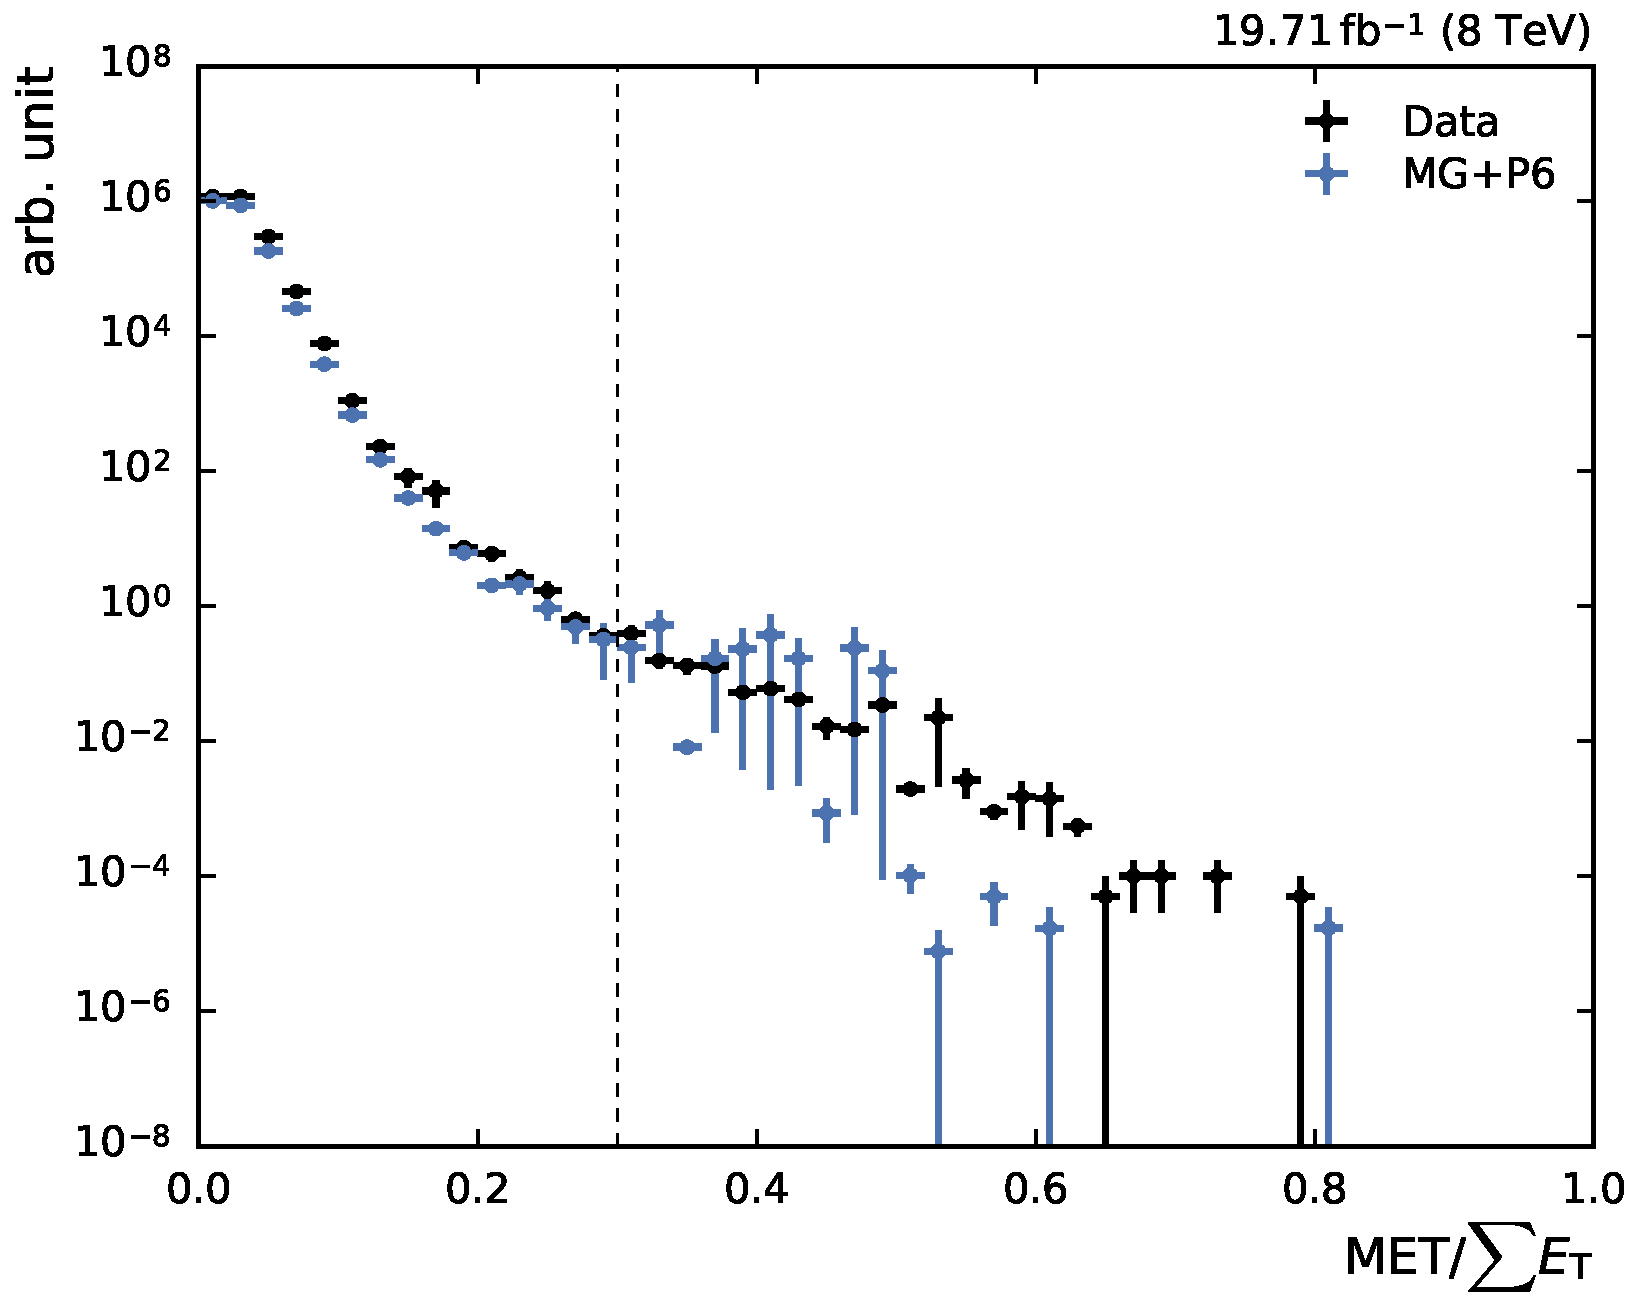
\includegraphics[width=0.5\textwidth]{figures/measurement/metoversumet.pdf}
    \caption[Missing transverse energy distribution]{Missing transverse energy
    fraction of the total transverse energy per event in data and simulated
    events. To remove background and noise, events with a fraction exceeding a
    threshold are rejected. }
    \label{fig:mc:met_fraction}
\end{figure}

A large fraction of the MET is not always caused by physics processes. Very
often the reason can be found in detector noise, cosmic rays or beam-halo
particles. Therefore there are a sequence of algorithms developed by the MET
working group at CMS identifying and rejecting these events. Additionally a cut
was introduced which removes events in which the missing transverse energy
fraction \met constitutes a large fraction of the total transverse energy, see
Fig.~\ref{fig:mc:met_fraction}.

\begin{equation}
    \frac{\met}{\sum_i E_{T,i}} < 0.3
\end{equation}


\subsection{Jet ID selection}

The jet identification criteria rejects noise and noise-enhanced
jets while keeping all real jets. The jet ID is not applied event-wise, but each
jet is accecpted or rejected by the jet id selection. The algorithm works on
particle flow jets using information of the underlying particles. 
Following the recommendations the official loose jet ID is used. Each jet
passing the jet id criteria is then further processed in the analysis chain. The
jet id criteria are based on the properties of each jet. The properties and the
respective cuts are listed in Table~\ref{tab:jetid}. The cut on the neutral
hadron and electromagnetic fractions removes HCAL and ECAL noise. Muons which
are falsely identified and clustered as jets are removed by the muon fraction
criterion. Based on information of the tracker, additional selection cuts are
enforced in the region $|\eta| < 2.4$. Fake jets clustered from electrons are
removed by the charged electromagnetic fraction cut and the charged hadron
fraction must be larger than zero.

While studying the loose and tight jet criteria, it was found that the tight jet
id removes a non-negligible fraction of jets in the forward region of the
phase space considered in this analysis. Therefore the loose jet id was applied.

\begin{table}[htbp]
    \centering
    \caption[Jet Identification Criteria]{The jet identification criteria remove fake jets originating from
    detector noise as well as wrongly clustered electrons and muons. Following
    the official recipe, the loose jet id was applied.}
    \label{tab:jetid}
    \begin{tabular}{llll}
    \toprule
                           & Property                & Loose ID & Tight ID\\\cmidrule(lr){2-4}
    Whole $\eta$ region    &                         &          & \\\cmidrule(lr){1-1}
                           & Neutral Hadron Fraction & $< 0.99$ & $< 0.90$\\
                           & Neutral EM Fraction     & $< 0.99$ & $< 0.90$\\
                           & Number of Constituents  & $> 1$    & $> 1$\\
                           & Muon Fraction           & $< 0.8$  & $< 0.80$\\
    Only $|\eta| < 2.4$    &                         &          & \\\cmidrule(lr){1-1}
                           & Charged Hadron Fraction & $> 0$    & $> 0$\\
                           & Charged Multiplicity    & $> 0$    & $> 0$\\
                           & Charged EM Fraction     & $< 0.99$ & $< 0.90$\\
    \bottomrule
    \end{tabular}
\end{table}


\subsection{Jet Selection}

The subsequent measurement is based on PFJet objects which are clustered
with the anti-\kt jet algorithm with a jet size parameter $R=0.7$. As discussed in
Section~\ref{sec:particle_flow_algorithm}, the input objects of the jet algorithm are not
calorimeter deposits but particles which are reconstructed by the Particle Flow
algorithms resulting in a superior performance compared to jets clustered only from
calorimeter deposits. 

Futhermore the CHS algorithm, detailed in Sec.~\ref{sec:chs_algorithm}, is used which effectively
reduces the influence of pile-up effects on jets.

All jets are corrected using the recommended jet energy corrections of CMS,
which relate the measured jet energy to the true particle jet energy. The
factorized approach employed by CMS is discussed in Sec.~\ref{sec:jec}. There are
distinct corrections for jets in data\footnote{The JEC version applied on data
    is internally referred to as \texttt{Winter14\_V8}} and for jets in simulated
events\footnote{The latest JEC for run-independent Monte Carlo Samples are
    called \texttt{START53\_V27}}.


The accessible phase space in theoretical calculations and the measurement is
synchronized by selecting jets only from a limited region of the complete phase
space. These selection cuts ensure a high detector efficiency as well as the
comparability of theory calculations with the measured cross sections.

\begin{align*}
    \ptjet &> \SI{50}{\GeV}\\
    |y_\mathrm{jet}| &\leq 3.0\\
    \ptavg &> \SI{133}{\GeV}
\end{align*}

The rapidity selection restricts the measurement to a phase space region without
detector inefficencies. In case the leading or second jet exceeds the rapidity
selection, not only the jet but the whole event is rejected. It is often
recommended to have asymmetric cuts on the transverse momentum of the two
leading jets to avoid an infrared sensitive region. This has no influence in
this cut due to the much higher cut on the average transverse momentum of dijet
system which results from the trigger thresholds of the employed jet triggers.
Another advantage of the high cut on \ptavg is the avoidance of a turn-on region
which can lead to complications in the unfolding procedure.

\subsection{Jet Pseudo-Rapidity Correction}
\todo{write}

\subsection{Stability versus Run Periods}
\todo{write}


\begin{figure}[htbp]
    \centering
    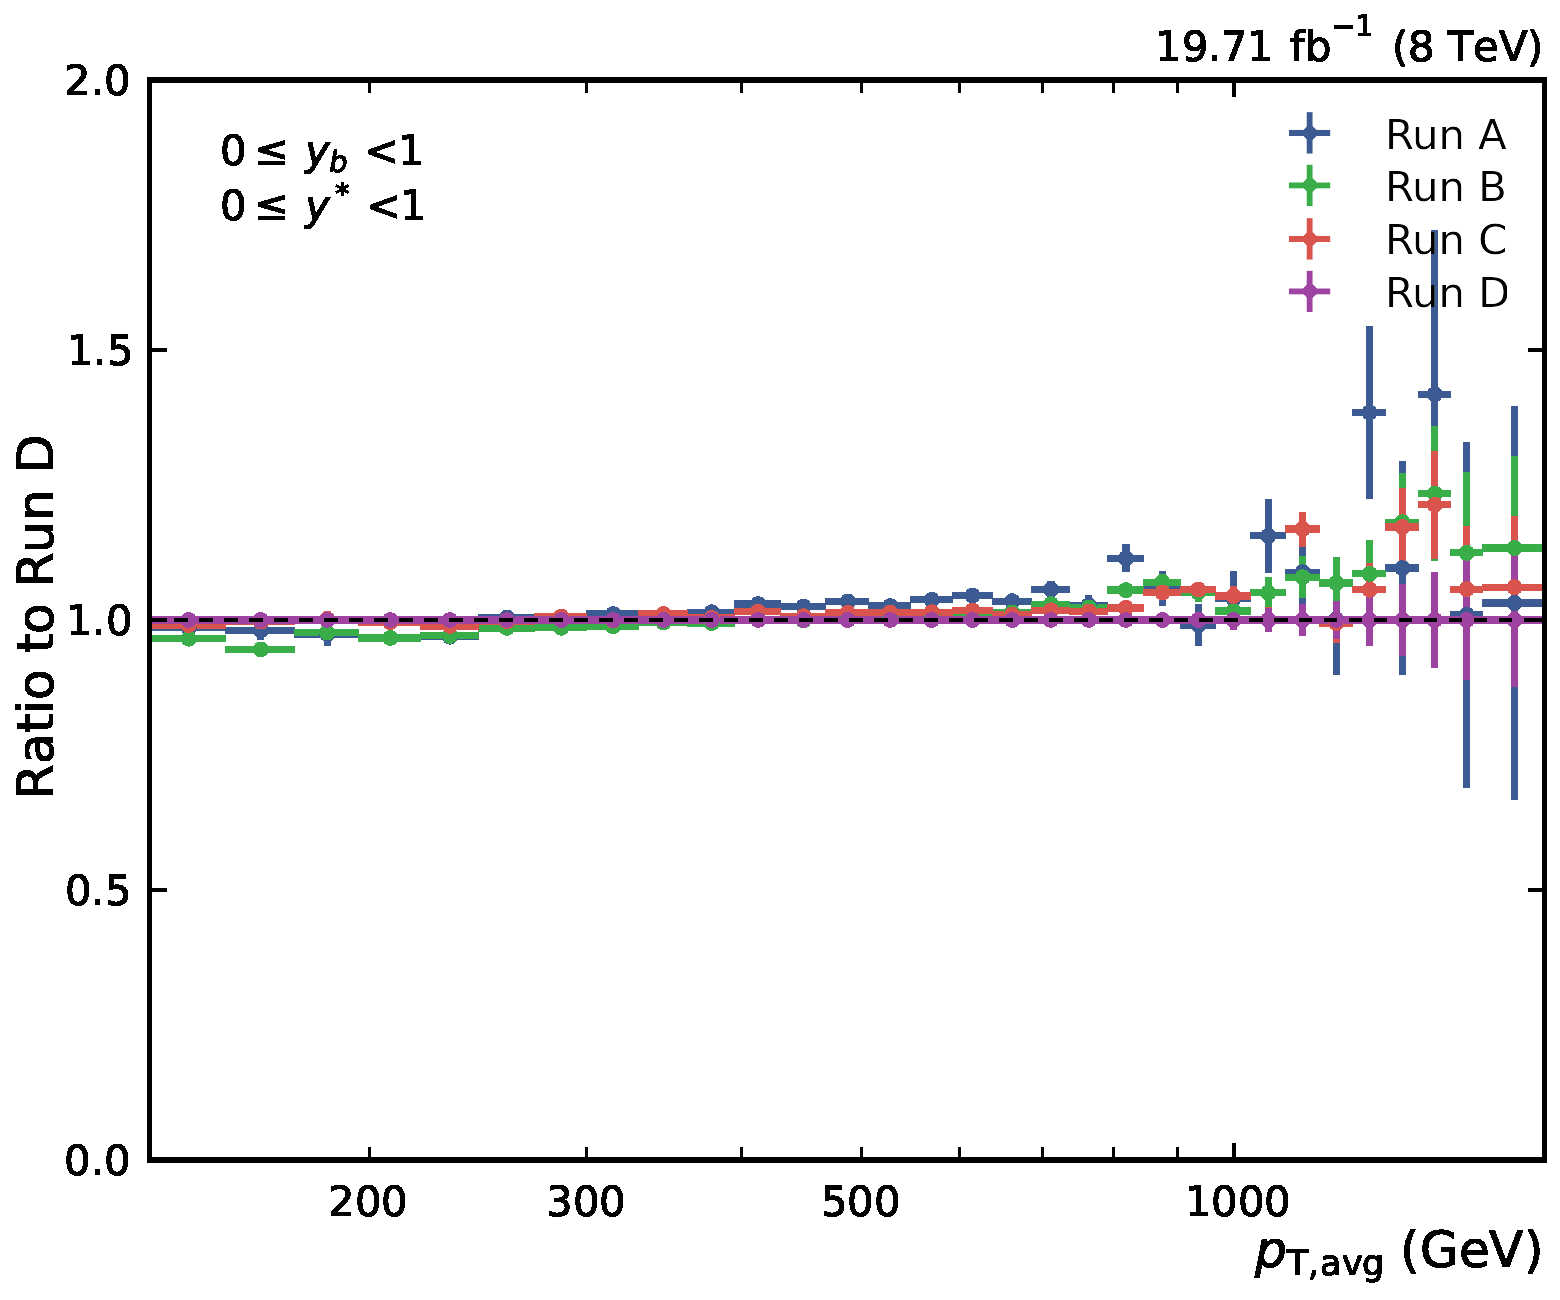
\includegraphics[width=0.45\textwidth]{figures/measurement/run_comparison_yb0ys0.pdf}\hfill
    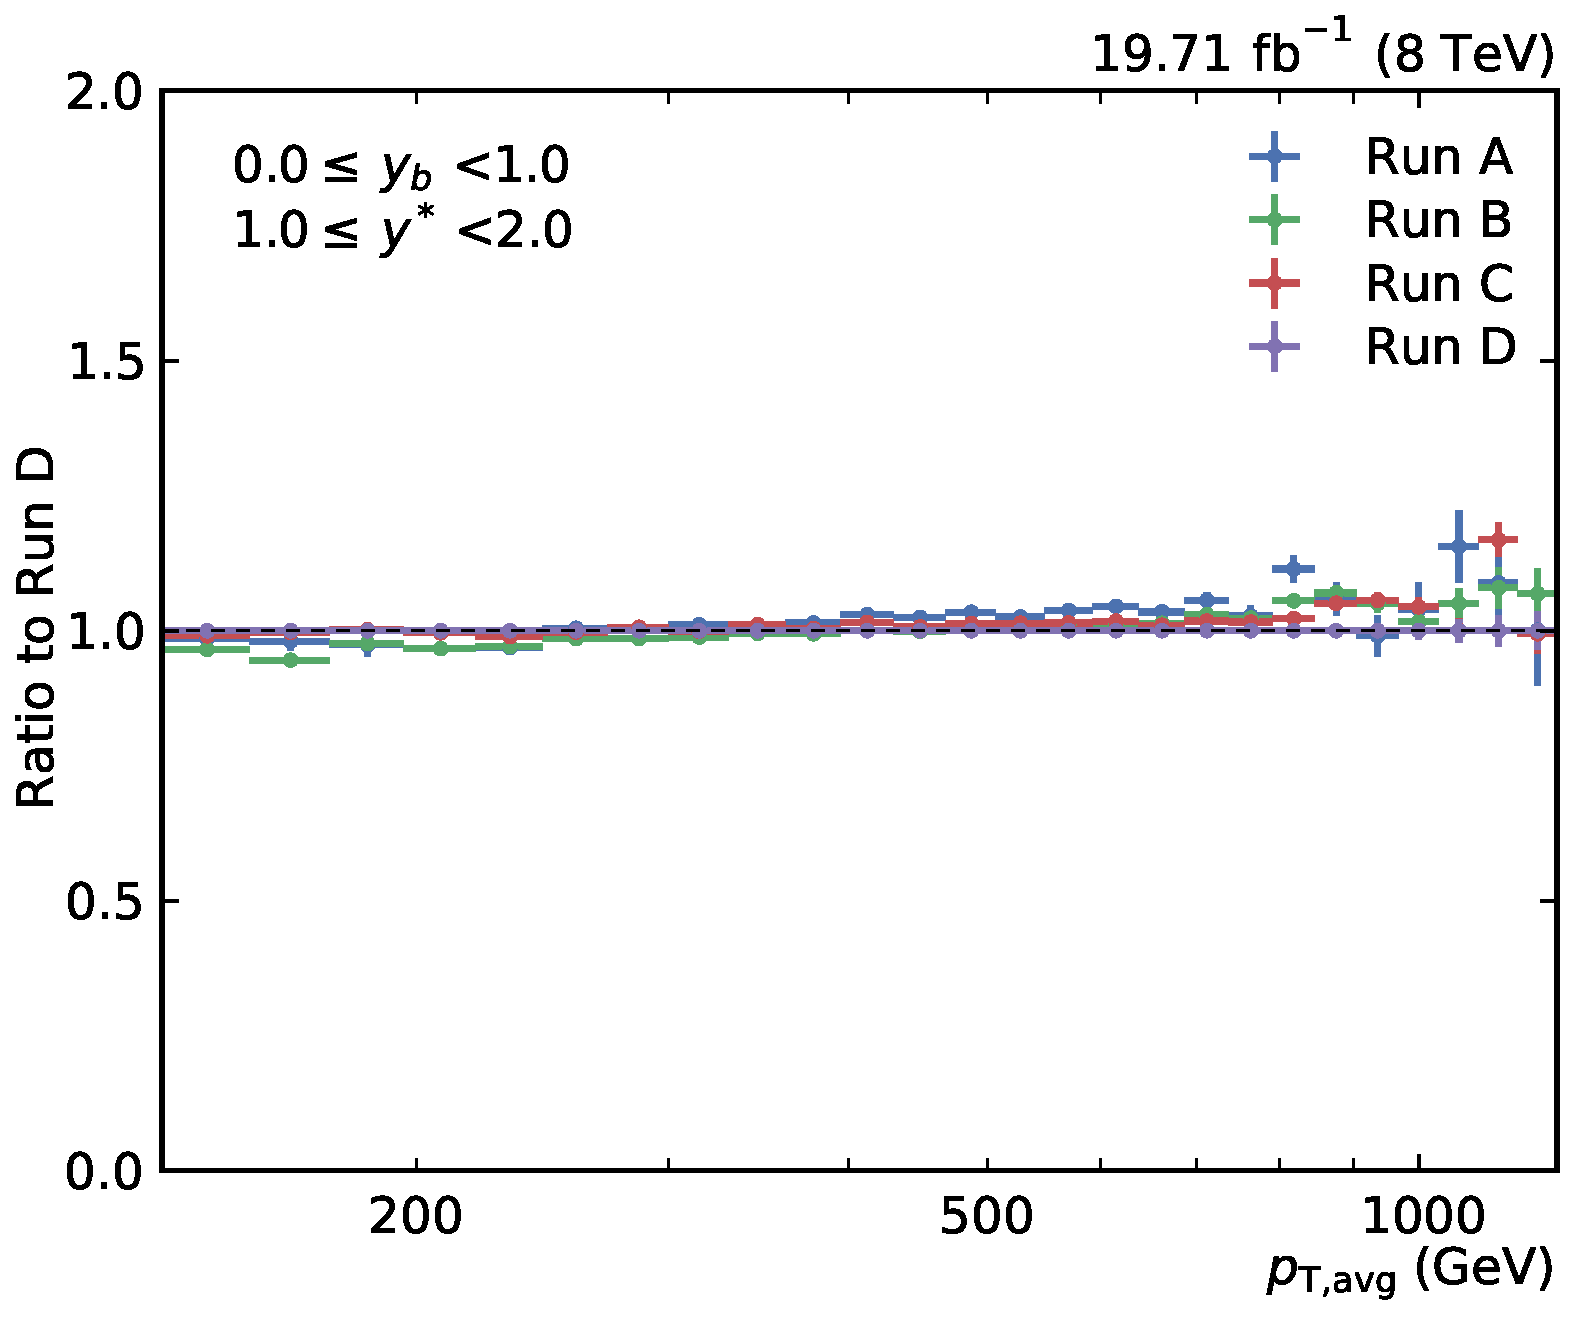
\includegraphics[width=0.45\textwidth]{figures/measurement/run_comparison_yb0ys1.pdf}
    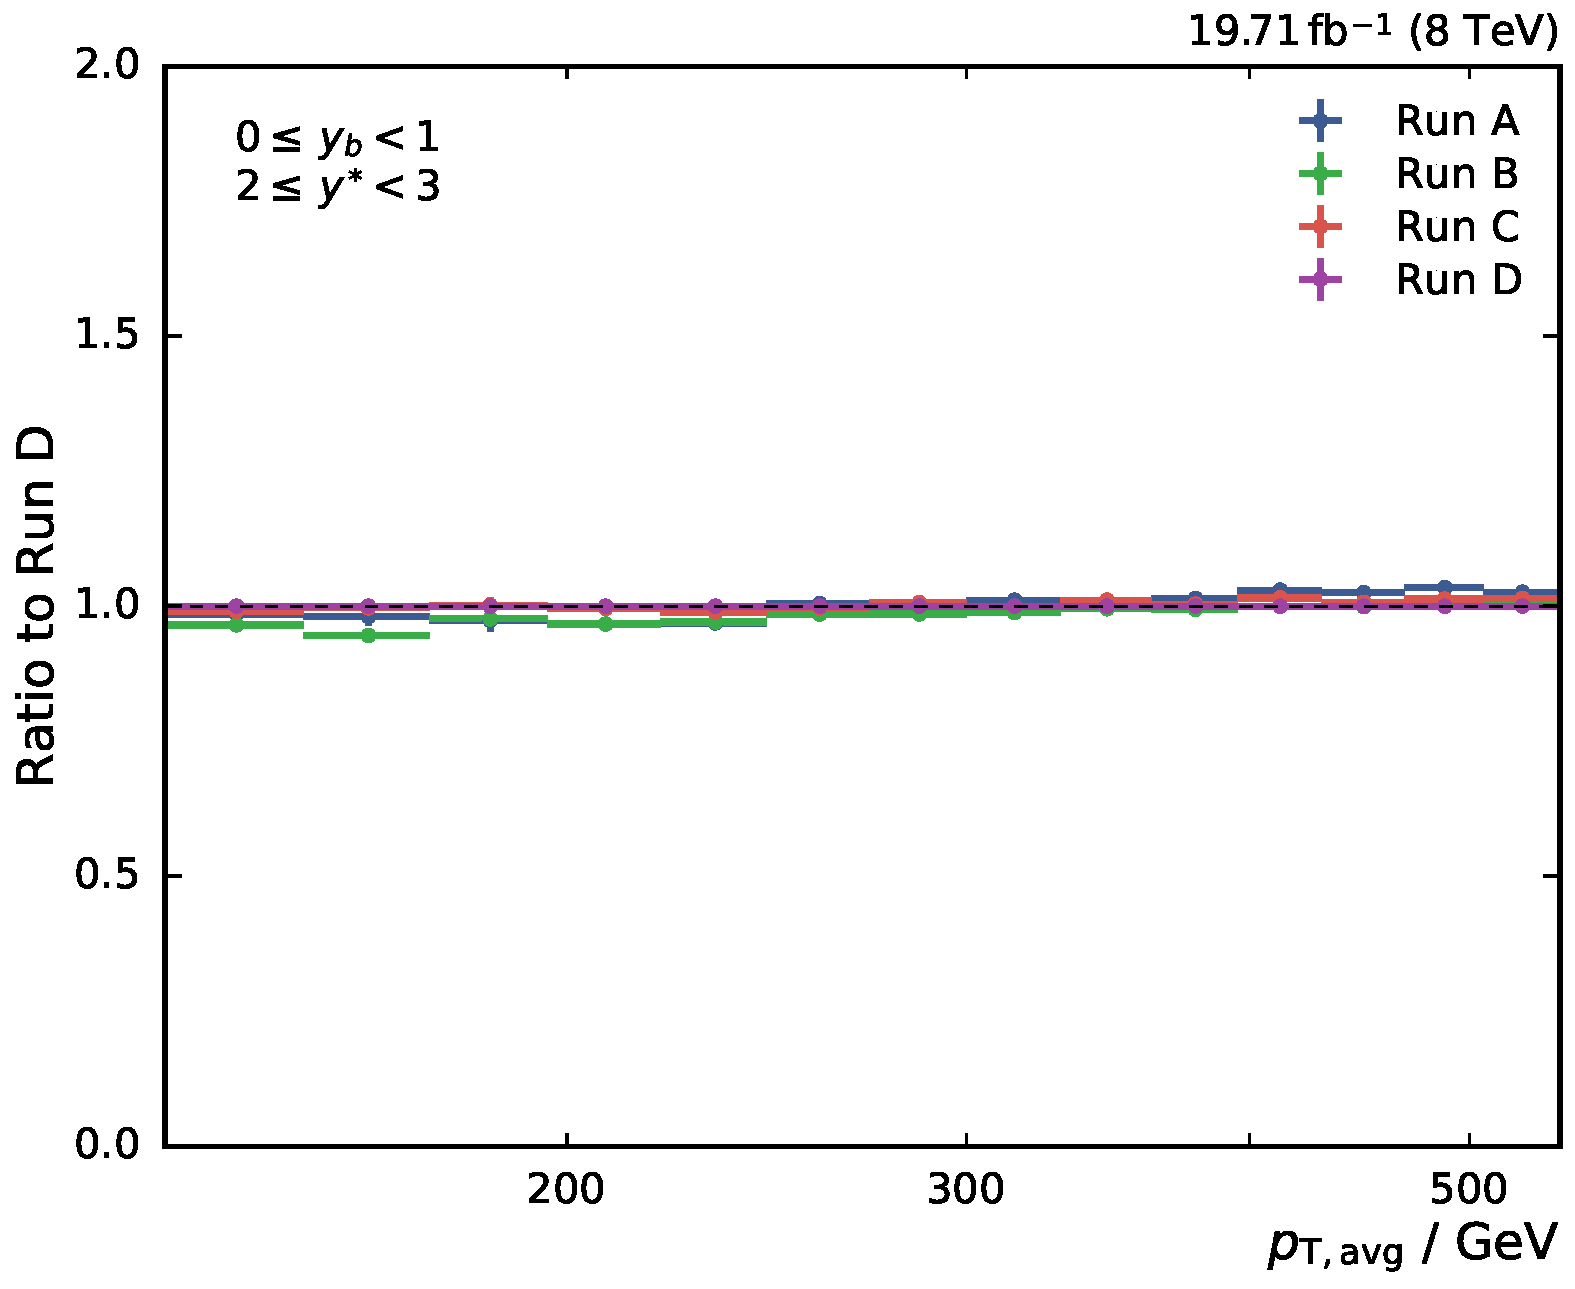
\includegraphics[width=0.45\textwidth]{figures/measurement/run_comparison_yb0ys2.pdf}\hfill
    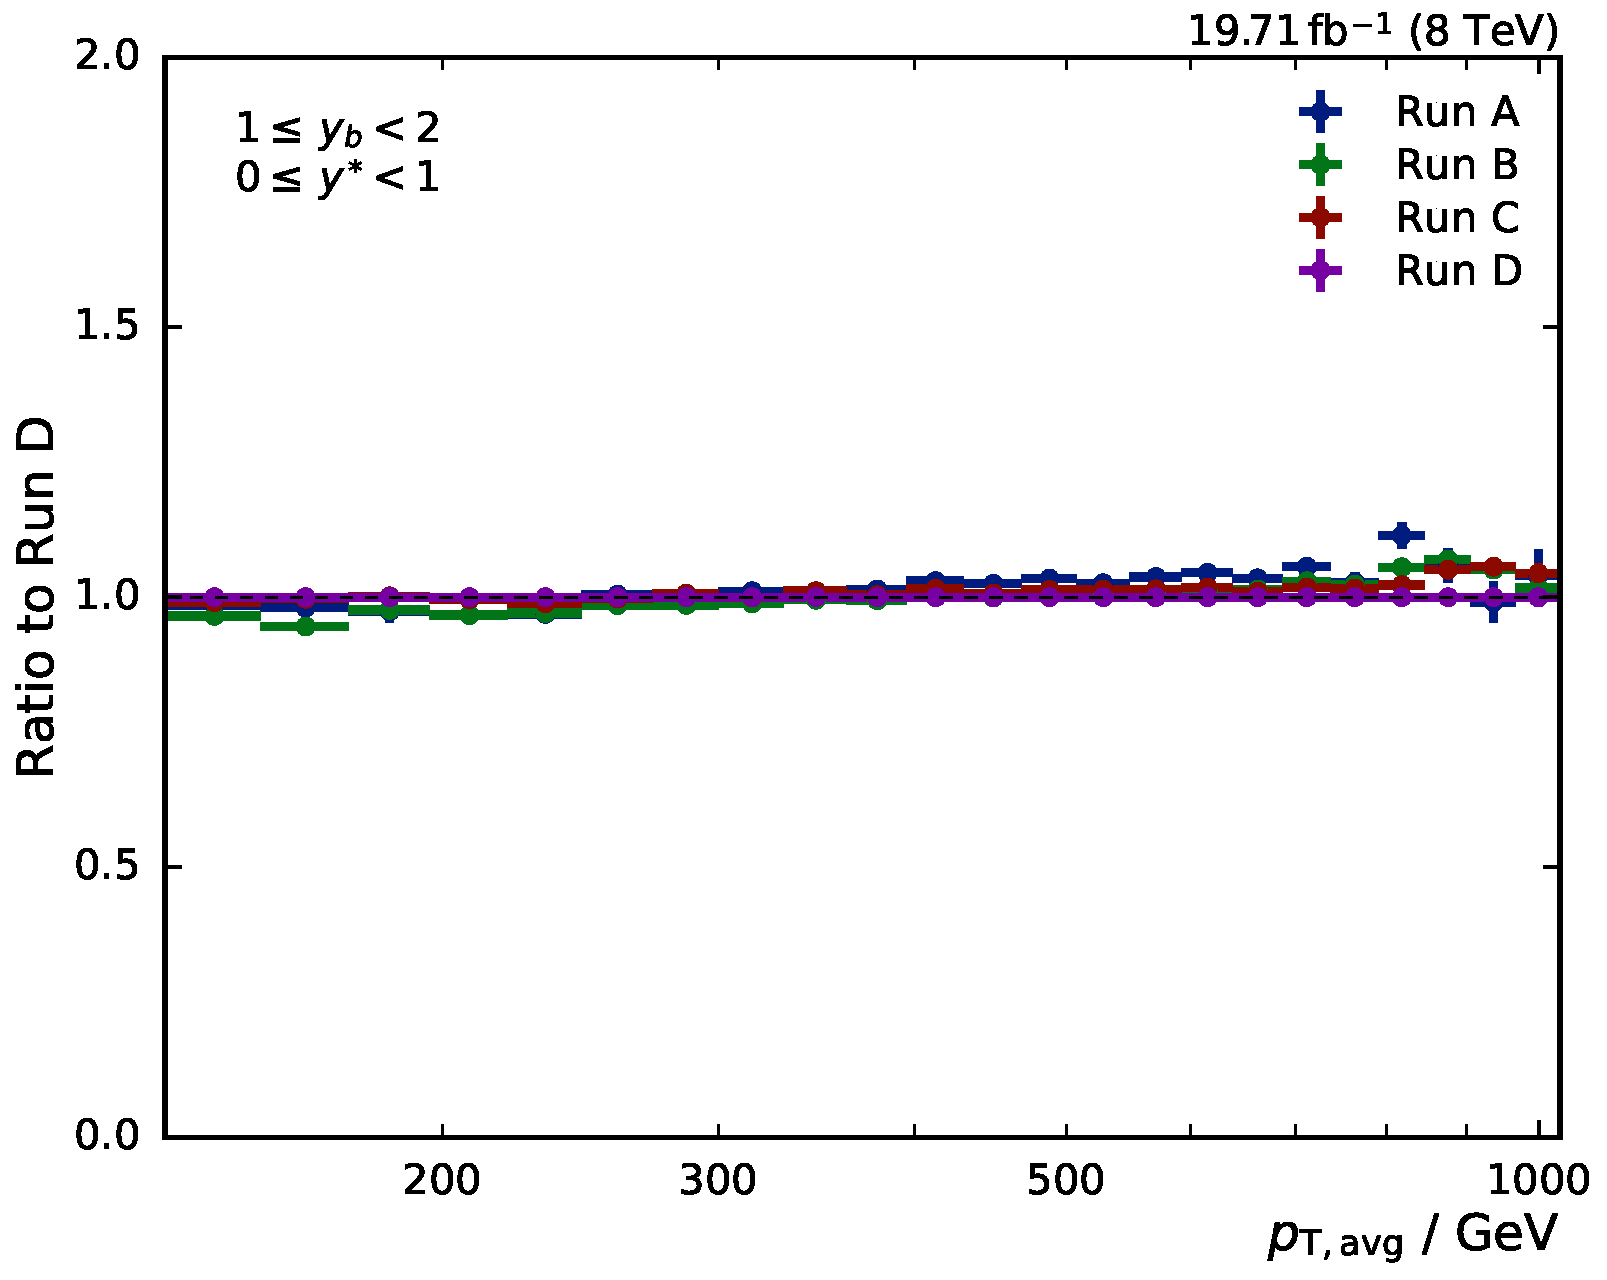
\includegraphics[width=0.45\textwidth]{figures/measurement/run_comparison_yb1ys0.pdf}
    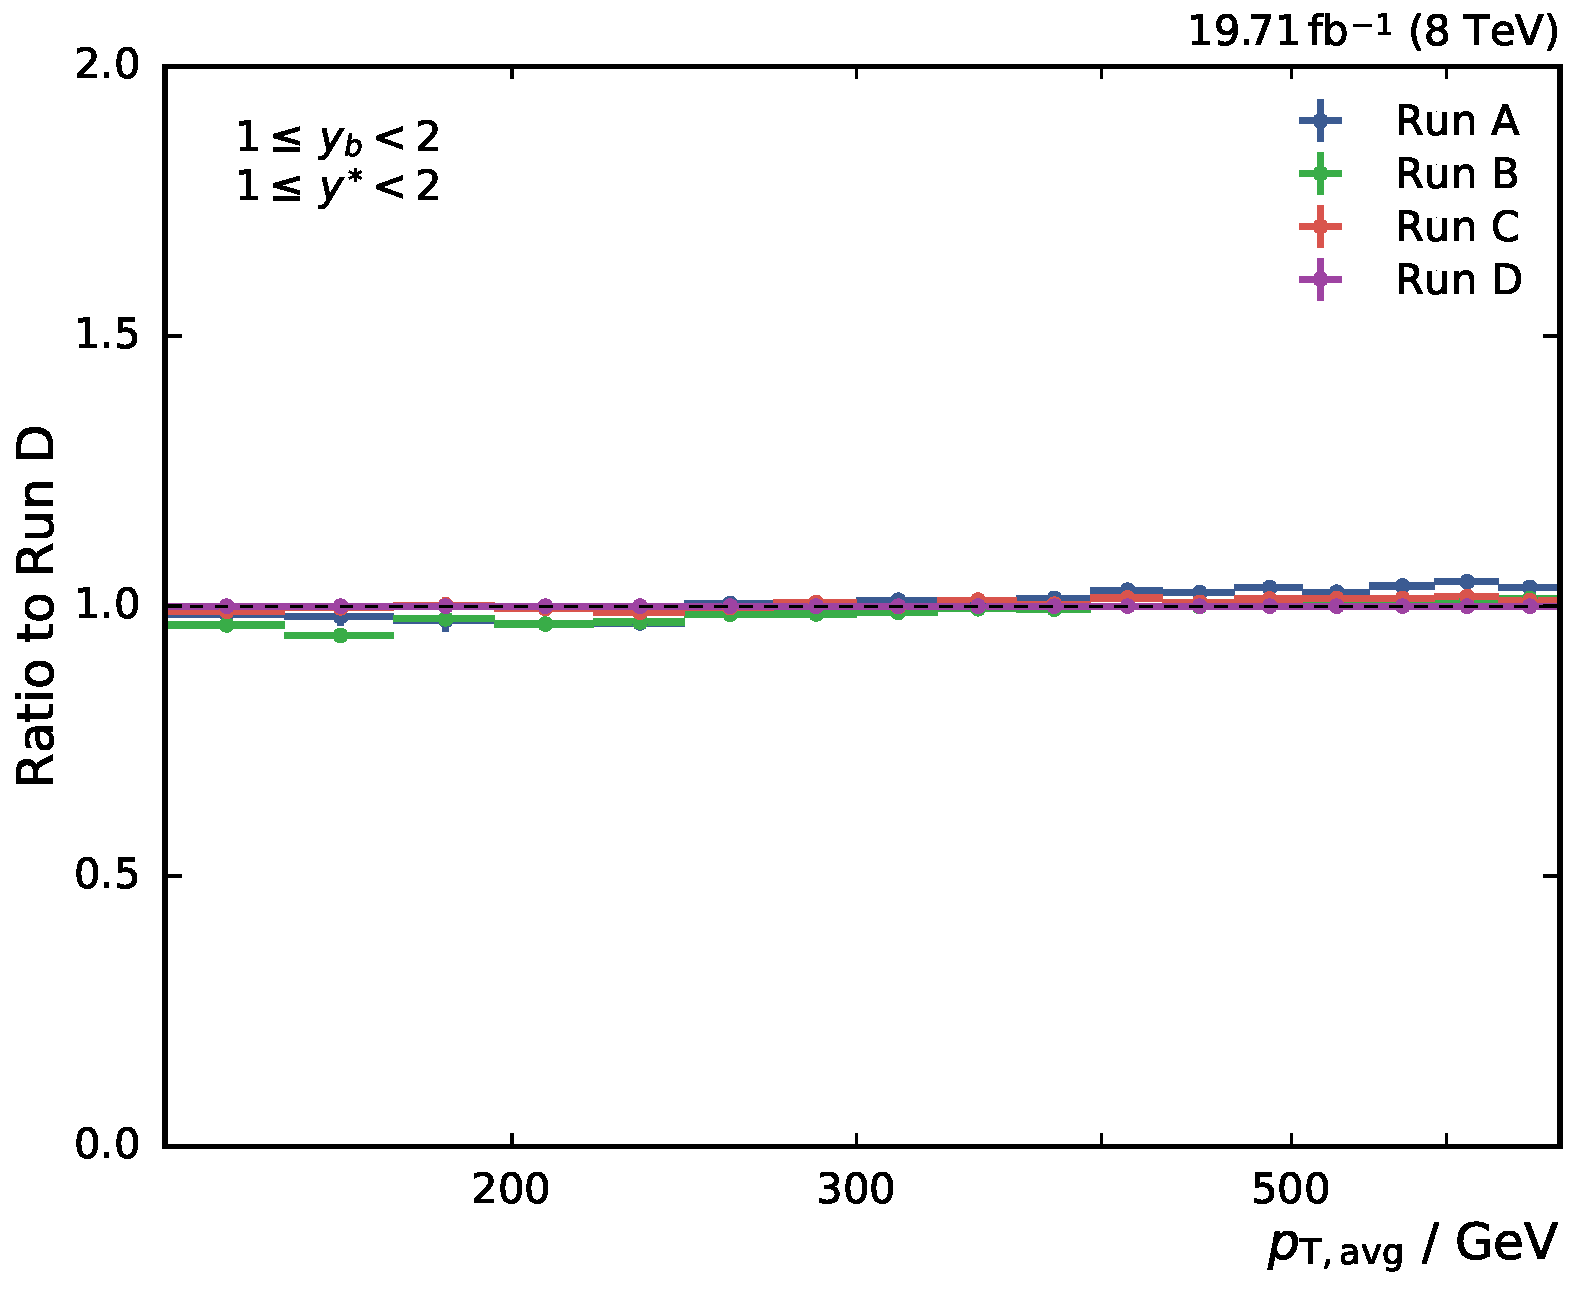
\includegraphics[width=0.45\textwidth]{figures/measurement/run_comparison_yb1ys1.pdf}\hfill
    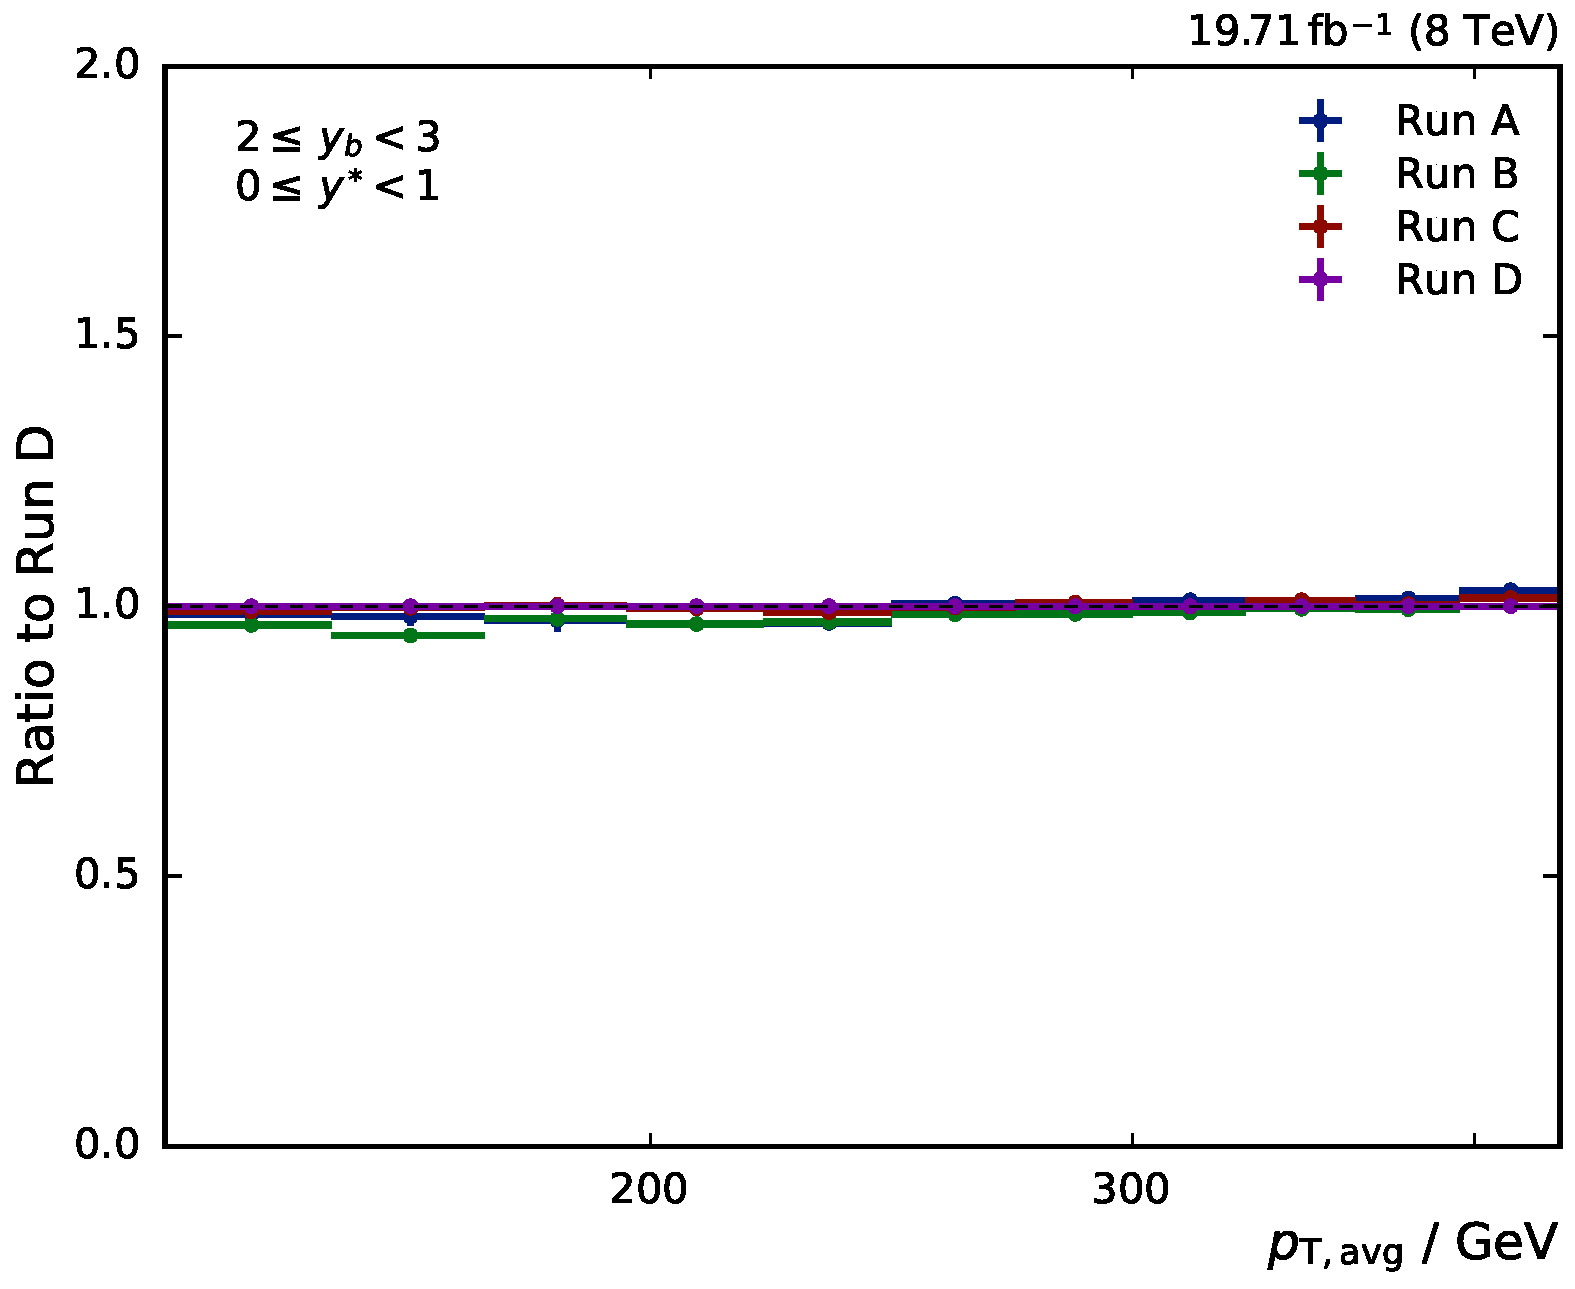
\includegraphics[width=0.45\textwidth]{figures/measurement/run_comparison_yb2ys0.pdf}
    \caption[Stability of result over all run periods]{Ratio of the measured
    cross section in each run period to the cross section in run period D. There
    are small differences, mostly due to statistical fluctuations. A slight slope is
    observed for the result of run B, but overall the differences are negligible.}
    \label{fig:run_comparison}
\end{figure}

\section{Comparison with Simulated Events}
\label{sec:simulated_events}

\subsection{Pile-up Reweighting}

The official Monte-Carlo samples are enriched with an admixture of pile-up to
mimic the pile-up distribution expected in data. Ideally the estimated pile-up
distribution in data $N_\mathrm{data} (N_\mathrm{PU, est.})$ would match with
the simulated distribution $N_\mathrm{MC} (N_\mathrm{PU, truth})$. Since the
admixture is only a rough estimate of the pile-up distribution expected in the
forthcoming data taking, a perfect matching cannot be achieved. To still get
comparable pile-up distributions in data and simulated events, the simulated
events are reweighted with a weight $w_\mathrm{PU}$ to match the distribution in
data: 

\begin{equation*}
    w_{\mathrm{PU}} (N_{mathrm{PU, truth}}) = \frac{N_\mathrm{data}
    (N_\mathrm{PU, est.}) / \sum N_\mathrm{data}}{N_\mathrm{MC}
    (N_\mathrm{PU, truth}) / \sum N_\mathrm{MC}}
\end{equation*}


Fig.~\ref{fig:mc:npv_reweighting} shows the number of reconstructed vertices
before and after reweighting. The significant mismatch of the
pile-up distributions in data and simulated events, which can be observed before
the reweighting, completely vanishes.

\begin{figure}[htbp]
    \centering
    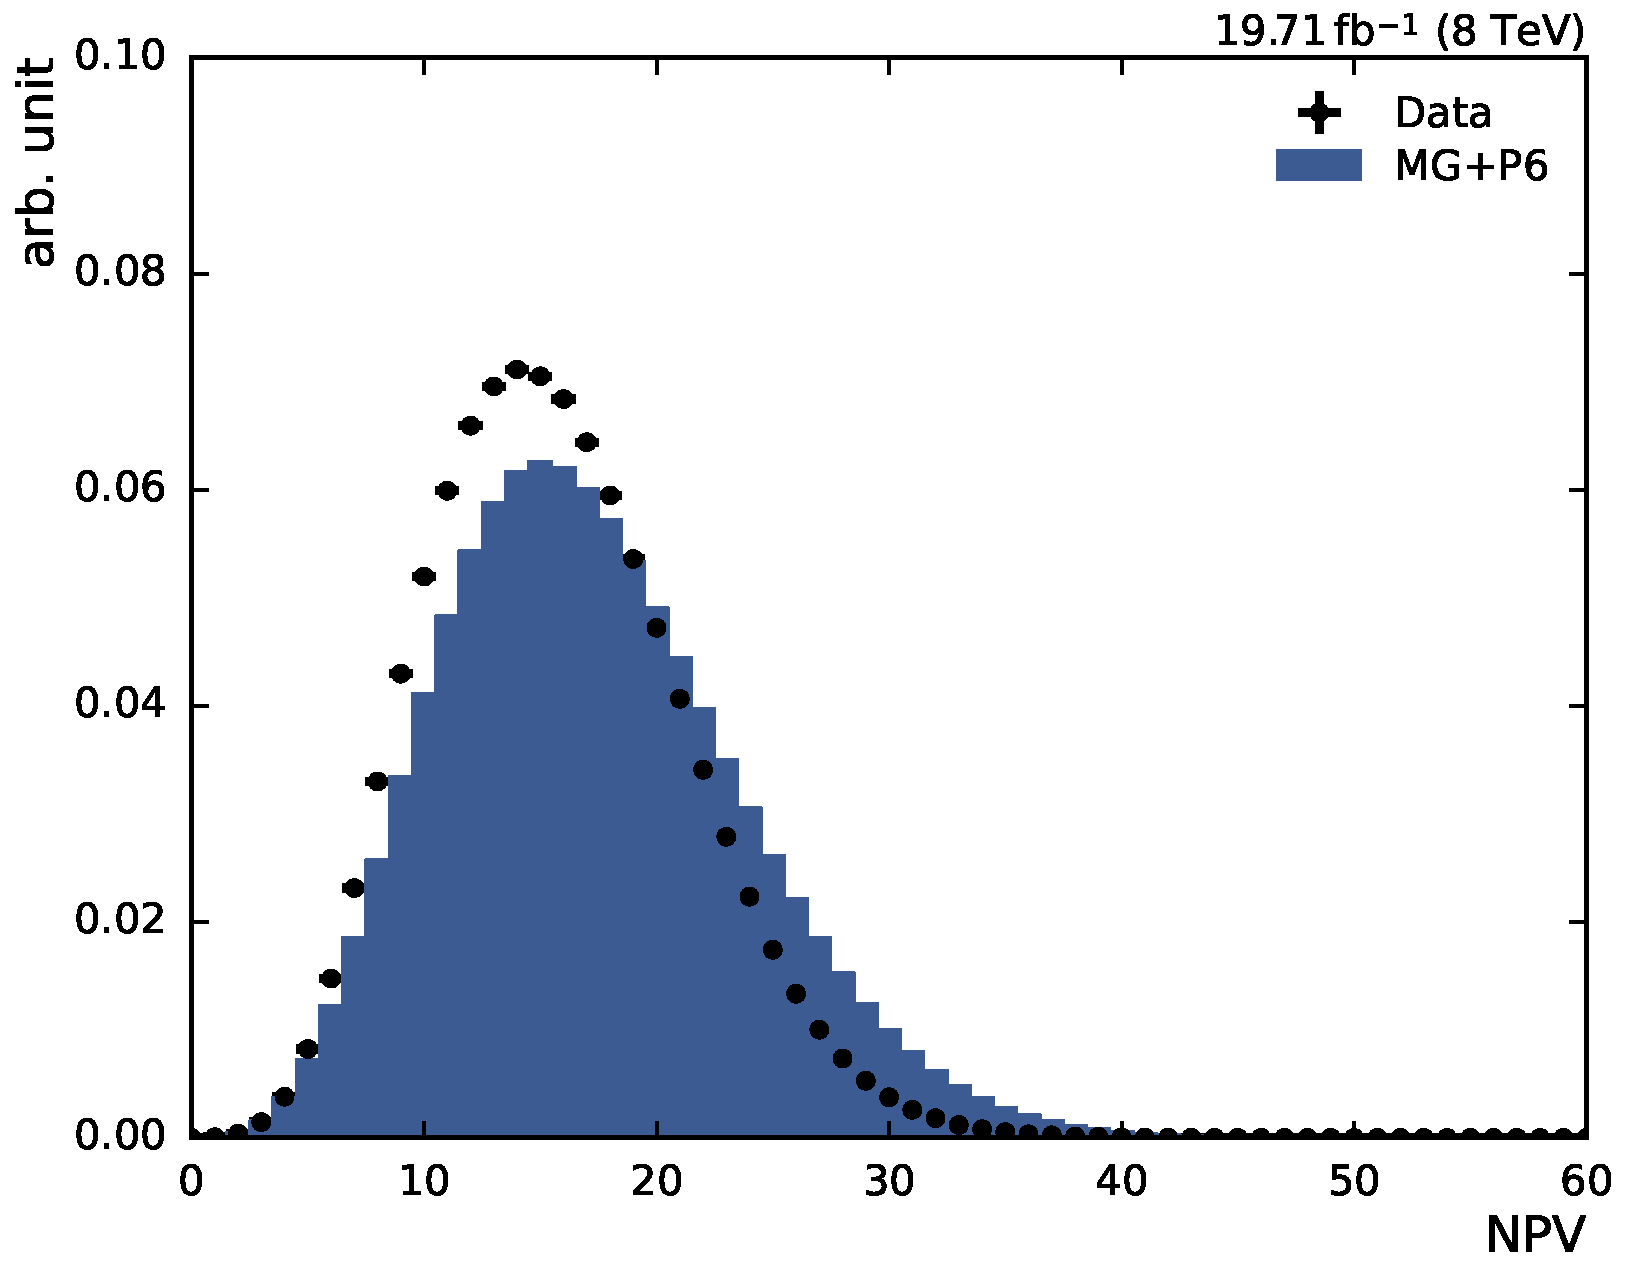
\includegraphics[width=0.49\textwidth]{figures/measurement/npv_beforereweighting.pdf}\hfill
    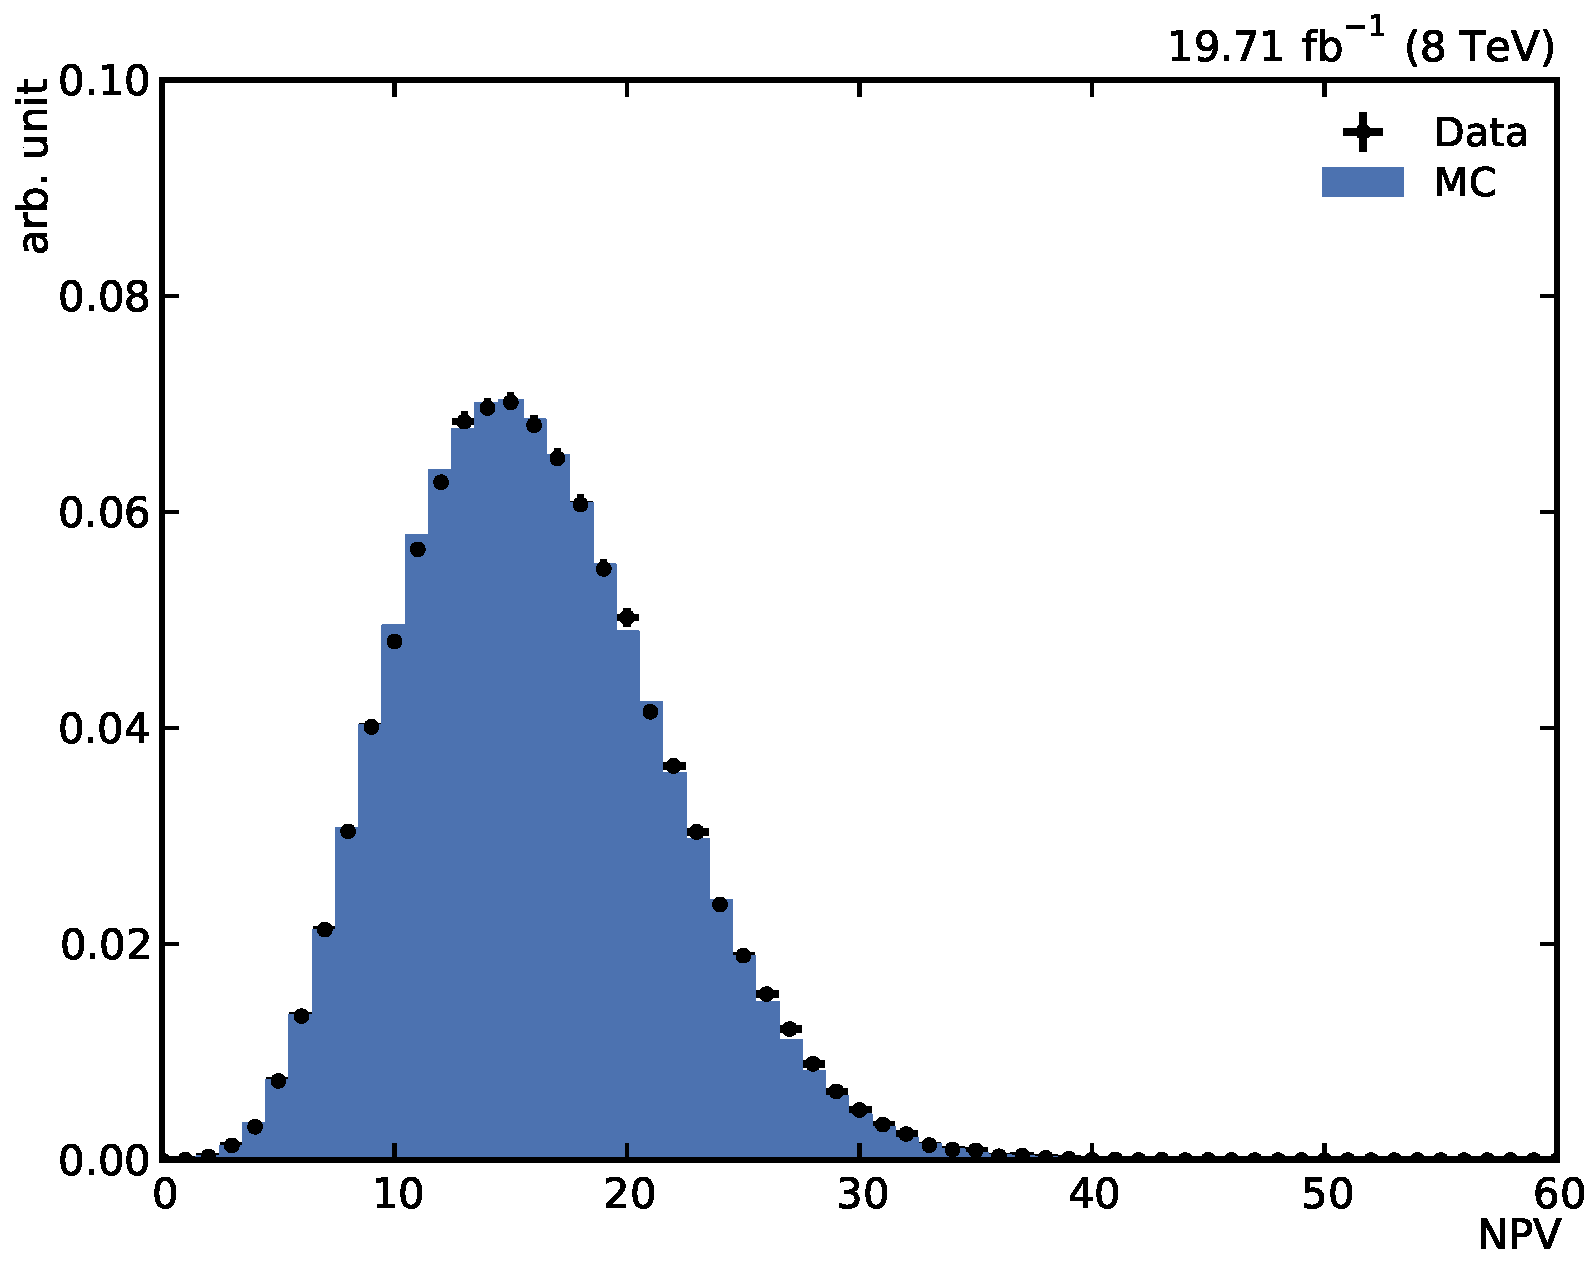
\includegraphics[width=0.49\textwidth]{figures/measurement/npv_afterreweighting.pdf}
    \caption[Number of reconstructed vertices]{Number of reconstruced vertices in data and simulated events before
    (left) and after (right) the pile-up reweighting.}
    \label{fig:mc:npv_reweighting}
\end{figure}

\subsection{Comparison of Kinematic Quantities}

The measured data distributions on detector level are compared with simulated events
processed through the whole event generation and detector simulation. In this section
the basic kinematic quantities of the leading two jets are compared as well as the properties
of each of the jets mainly describing the constituent fractions of each jet. Figure~\ref{fig:controlplots:kinematic}
shows the transverse momentum $\pt$, the rapidity $y$ and the azimuthal angle $\phi$ for the leading
two jets. The kinematic of the two dijet system is well described by the MC simulation apart from
a few regions with larger discrepancies. The \pt-distribution is not that well described escpecially in
the lower \pt region and the number of events with forward jets is overestimated in the MC simulation.

\begin{figure}[htbp]
    \centering
    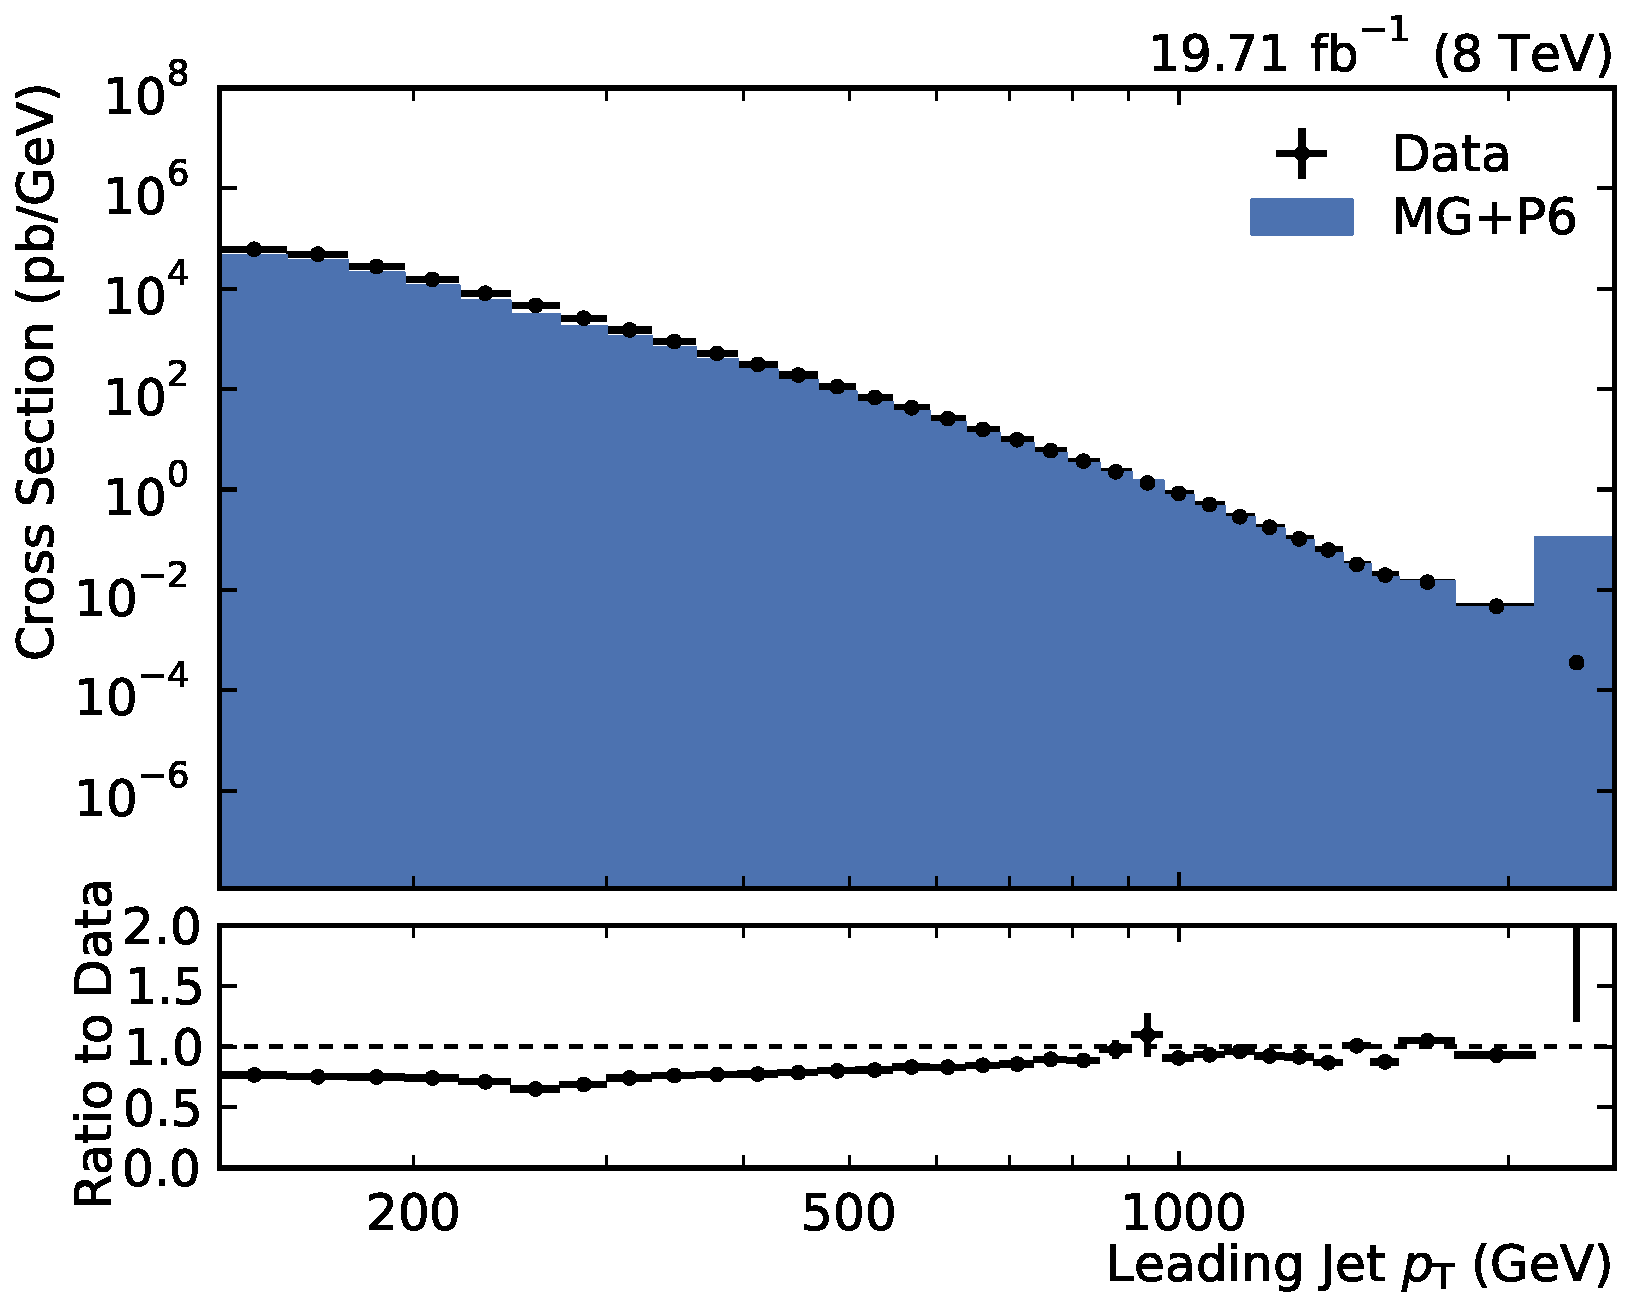
\includegraphics[width=0.45\textwidth]{figures/measurement/jet1pt_default.pdf}\hfill
    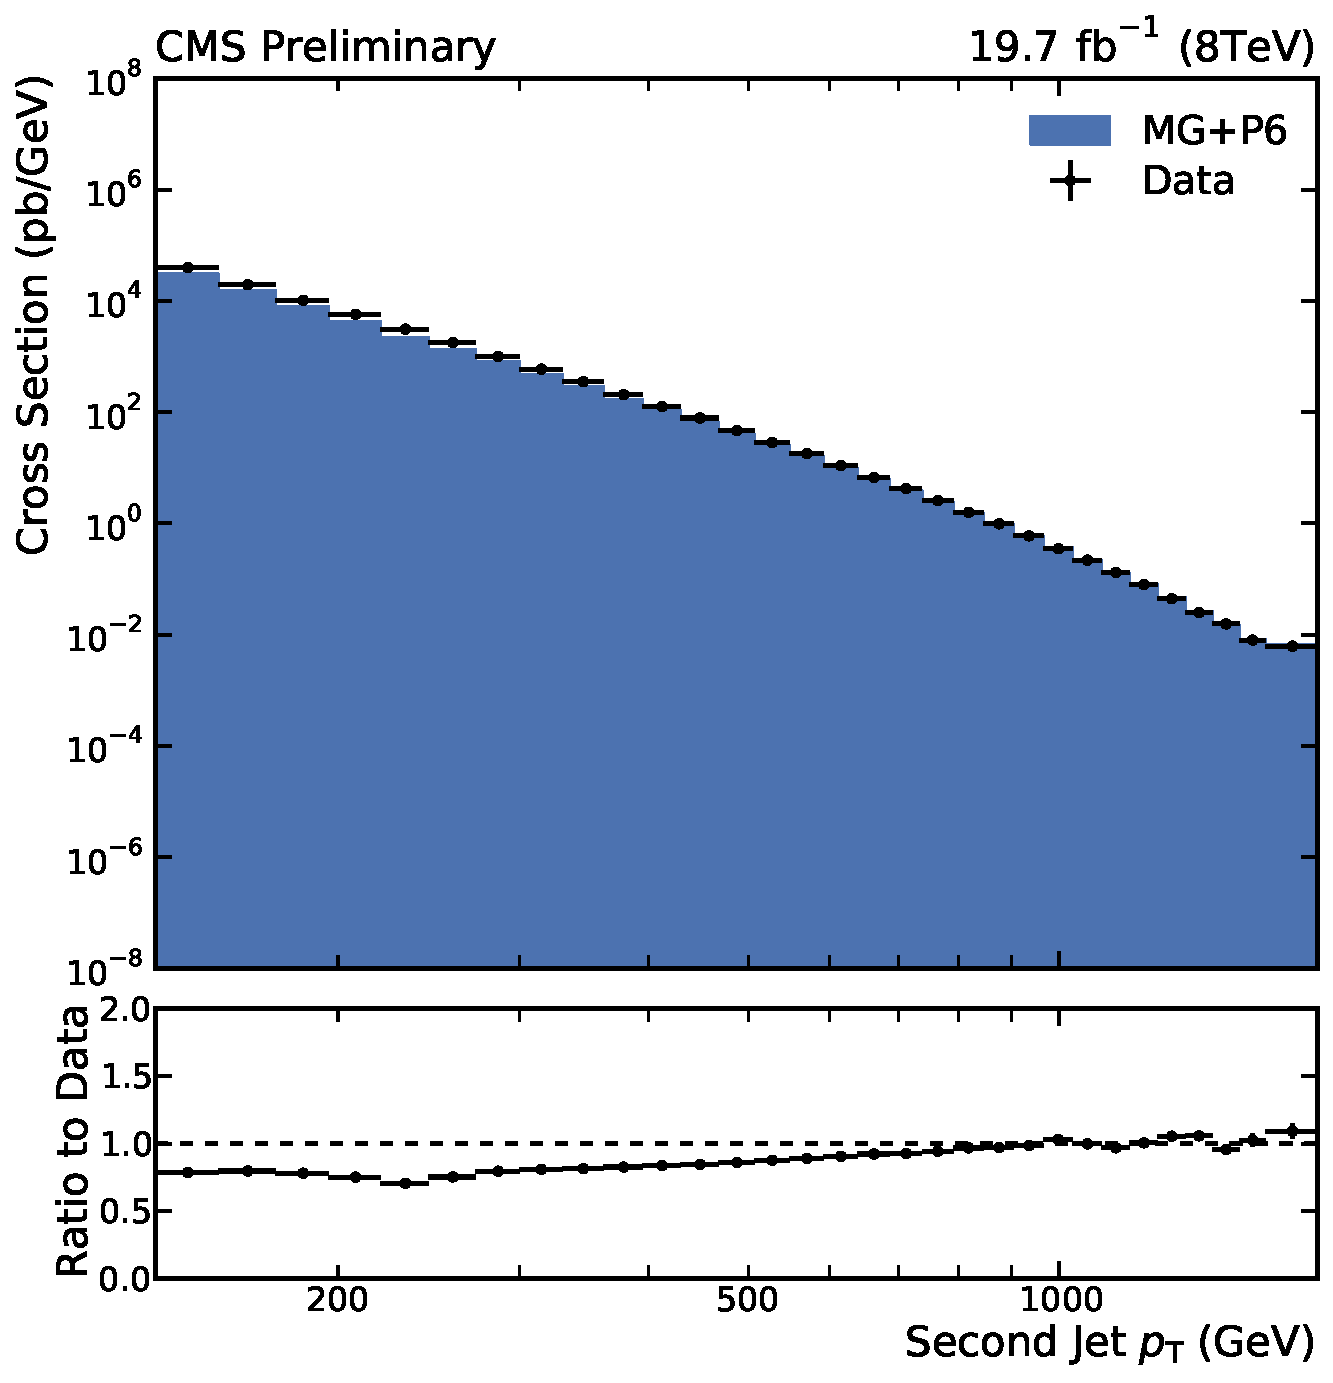
\includegraphics[width=0.45\textwidth]{figures/measurement/jet2pt_default.pdf}
    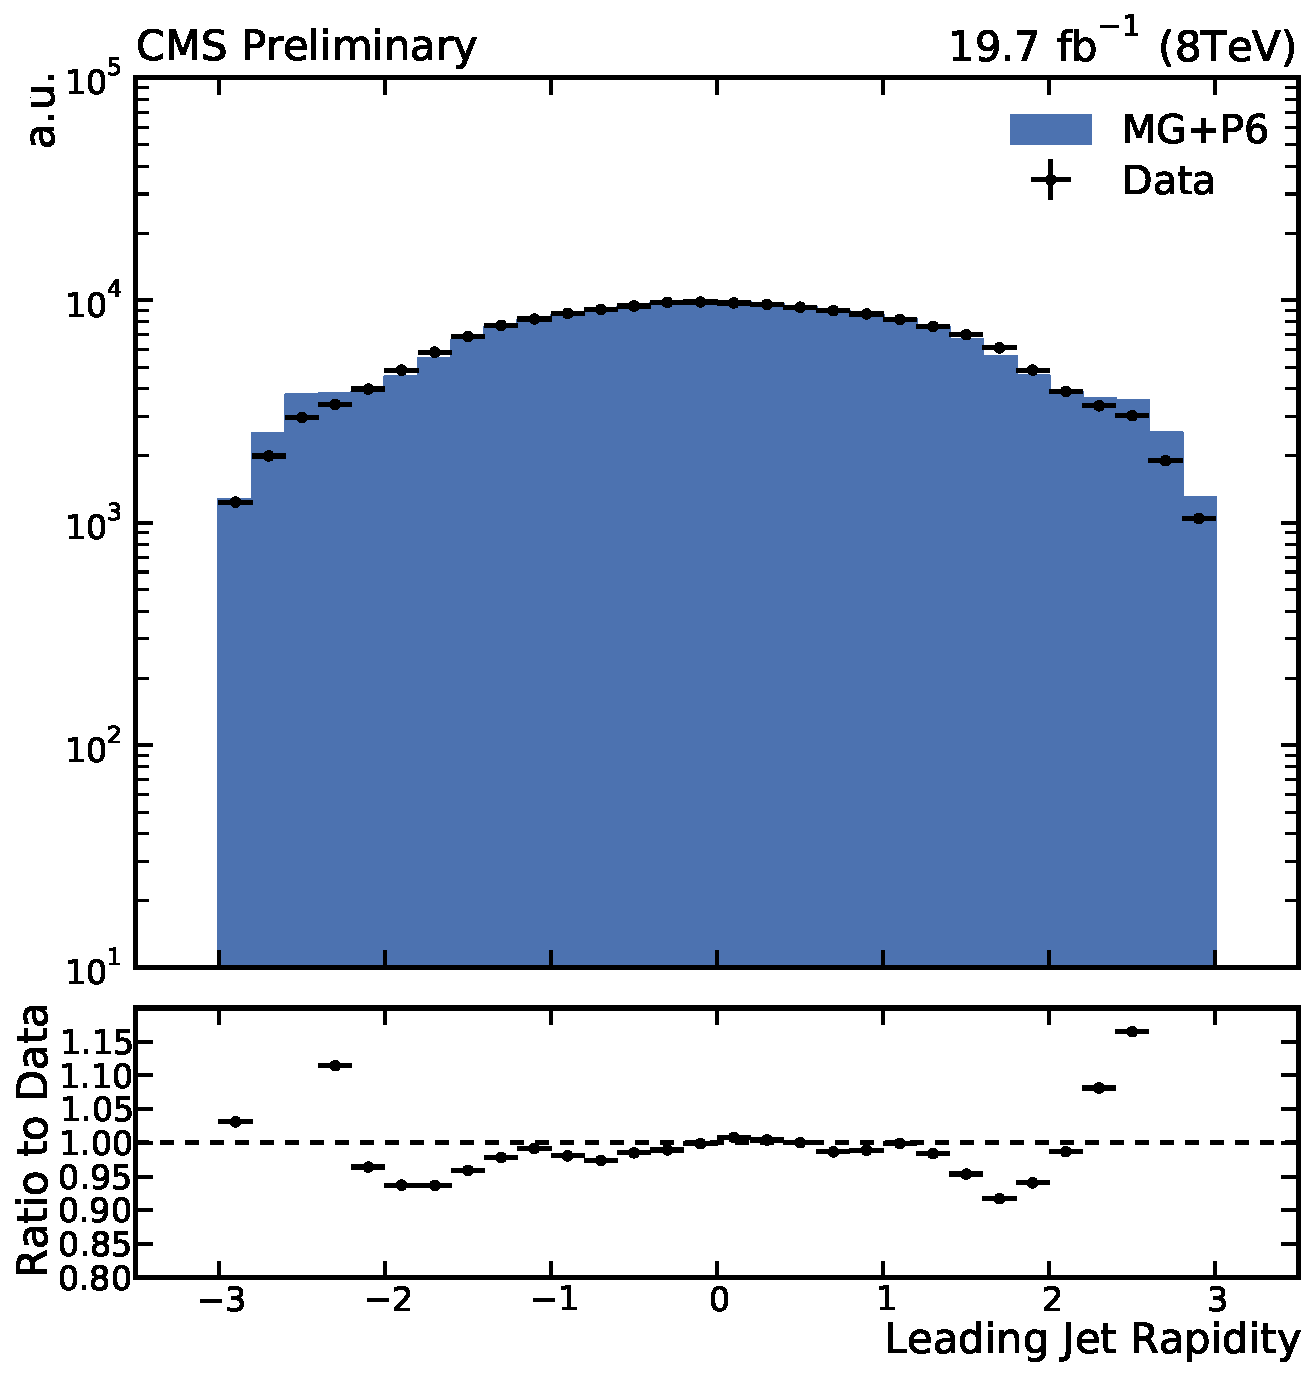
\includegraphics[width=0.45\textwidth]{figures/measurement/jet1rap_default.pdf}\hfill
    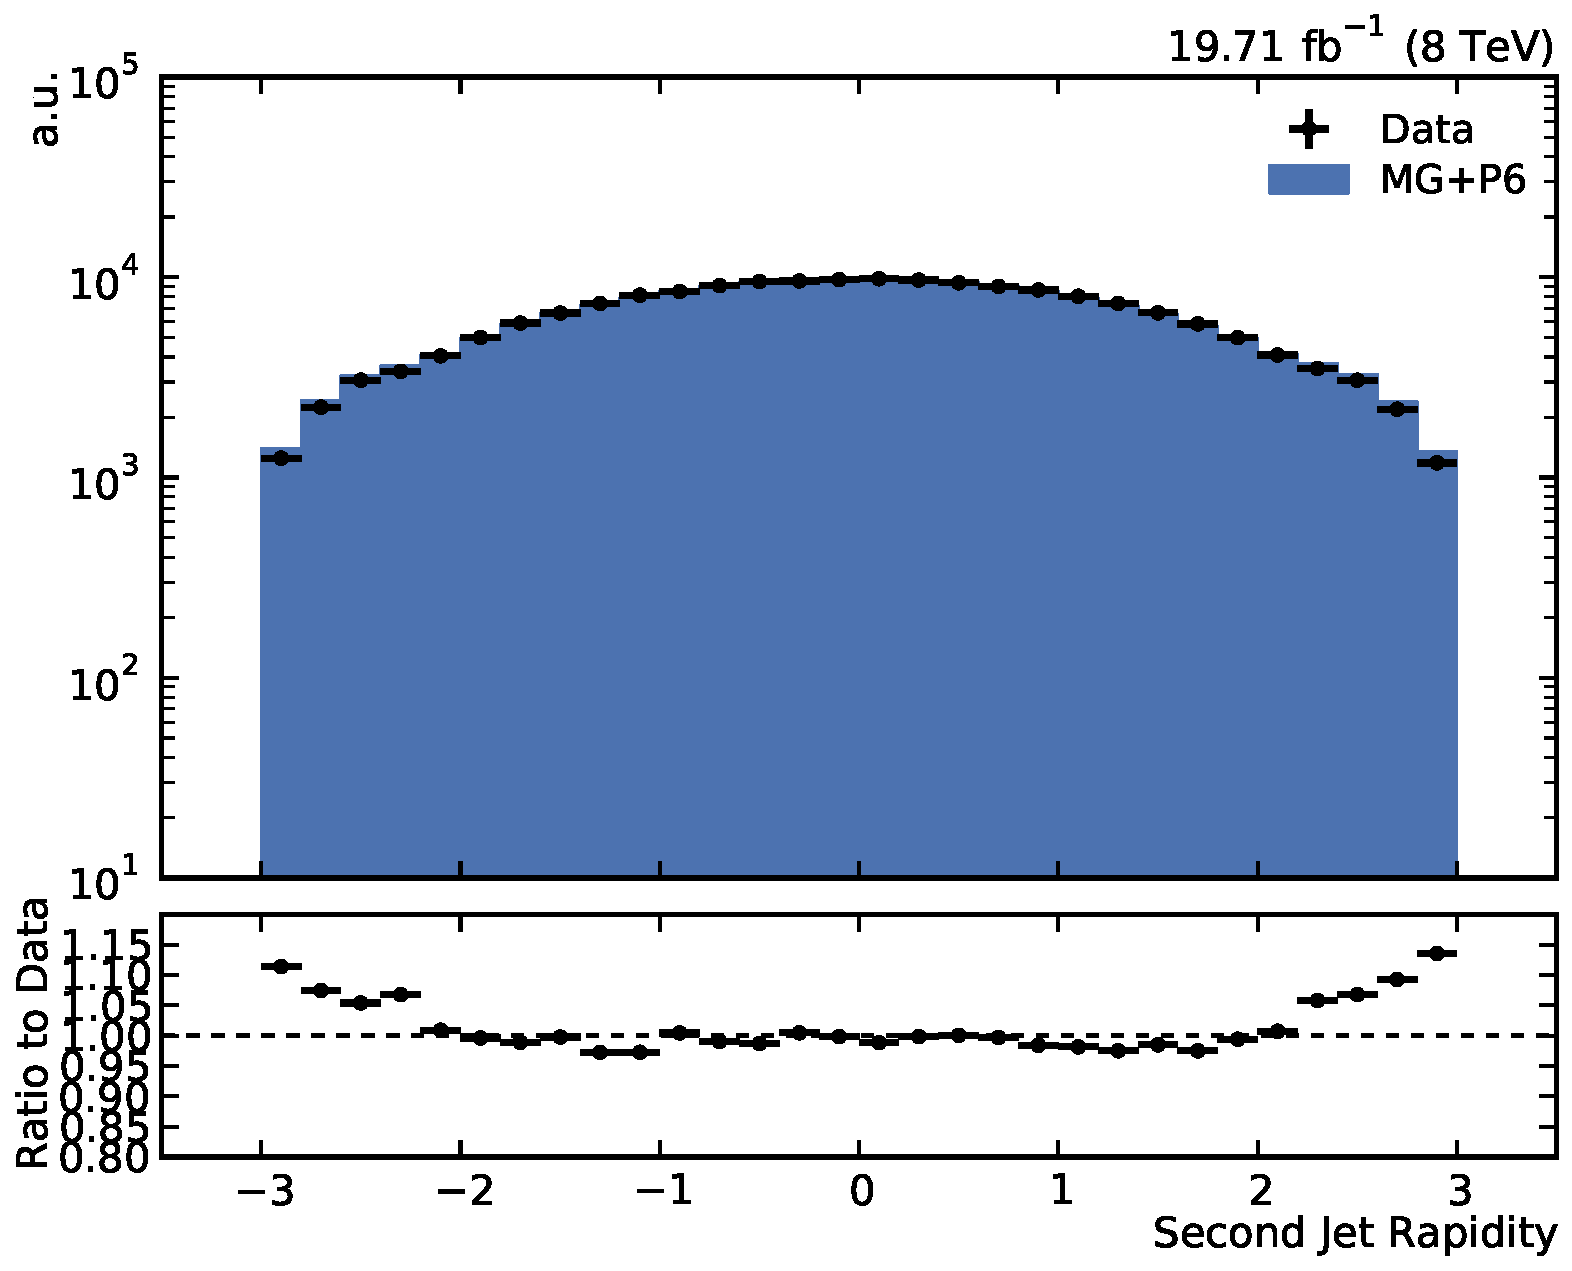
\includegraphics[width=0.45\textwidth]{figures/measurement/jet2rap_default.pdf}
    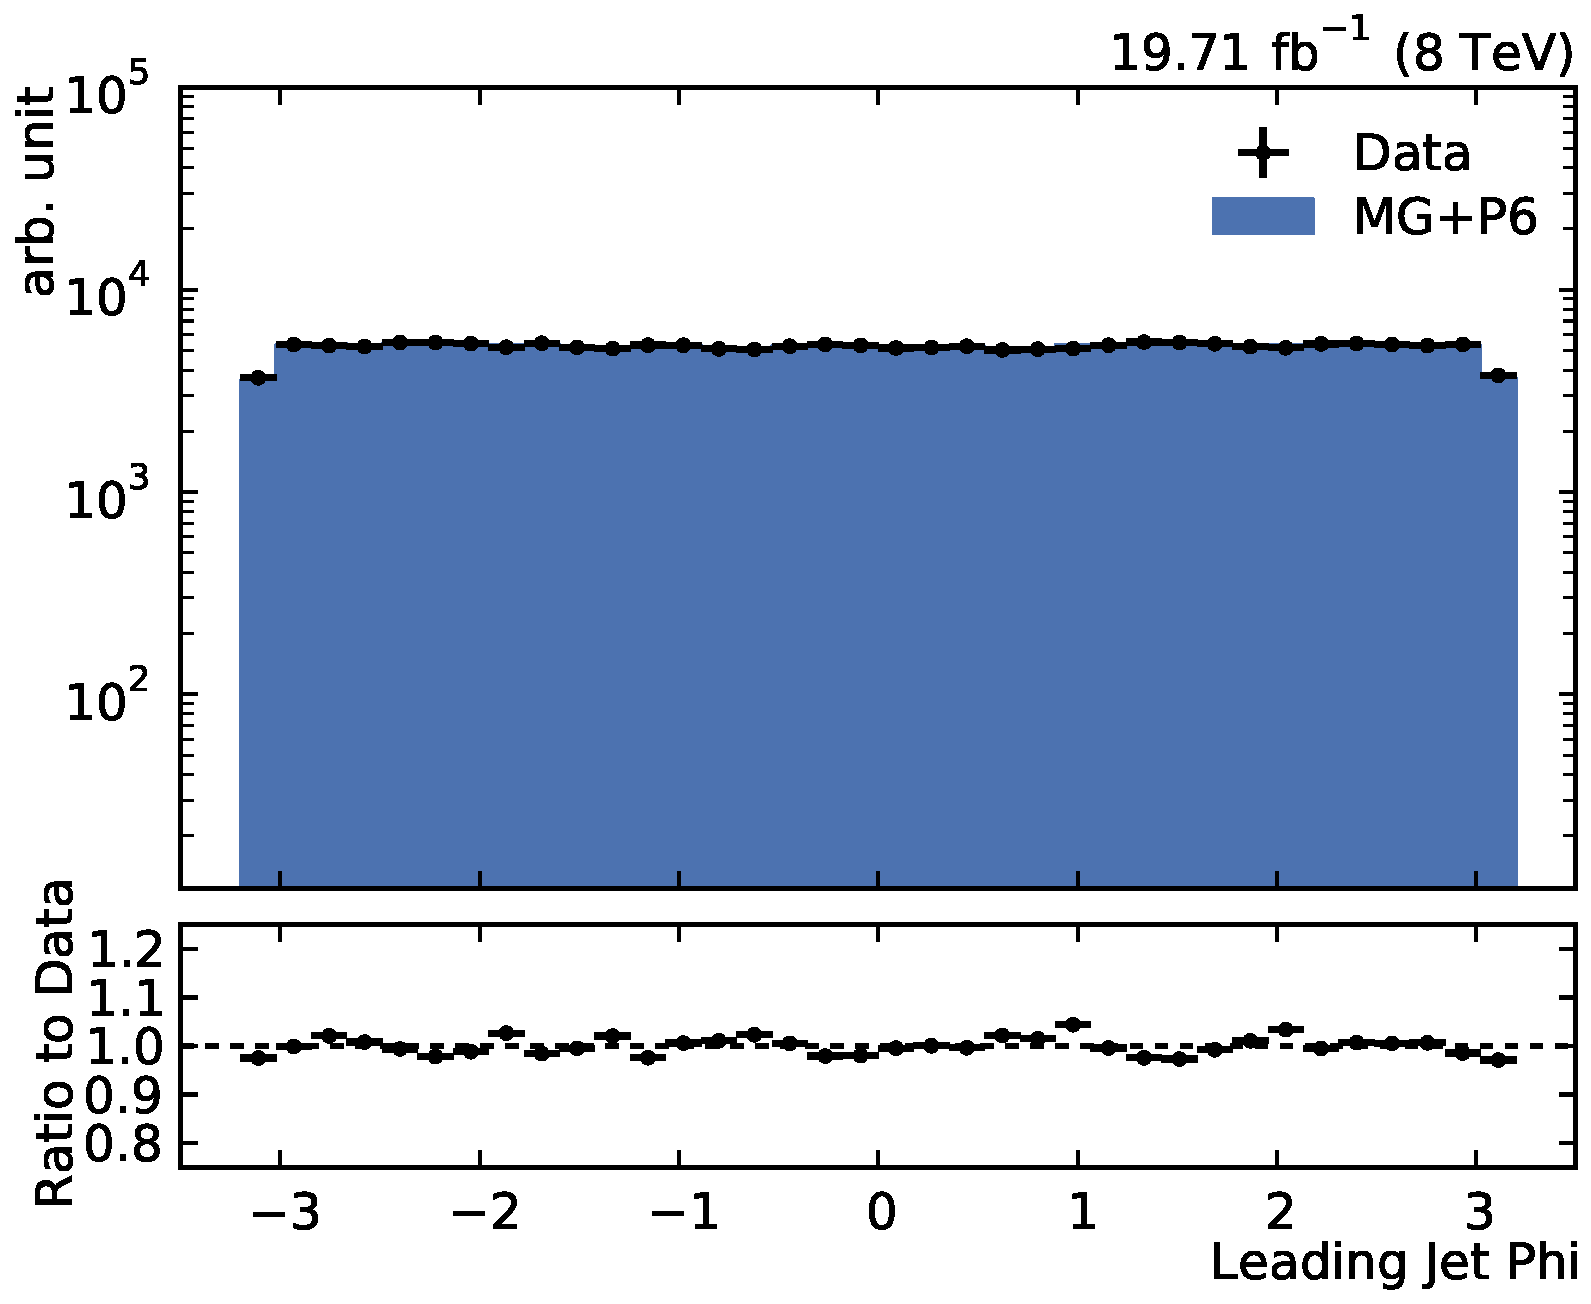
\includegraphics[width=0.45\textwidth]{figures/measurement/jet1phi_default.pdf}\hfill
    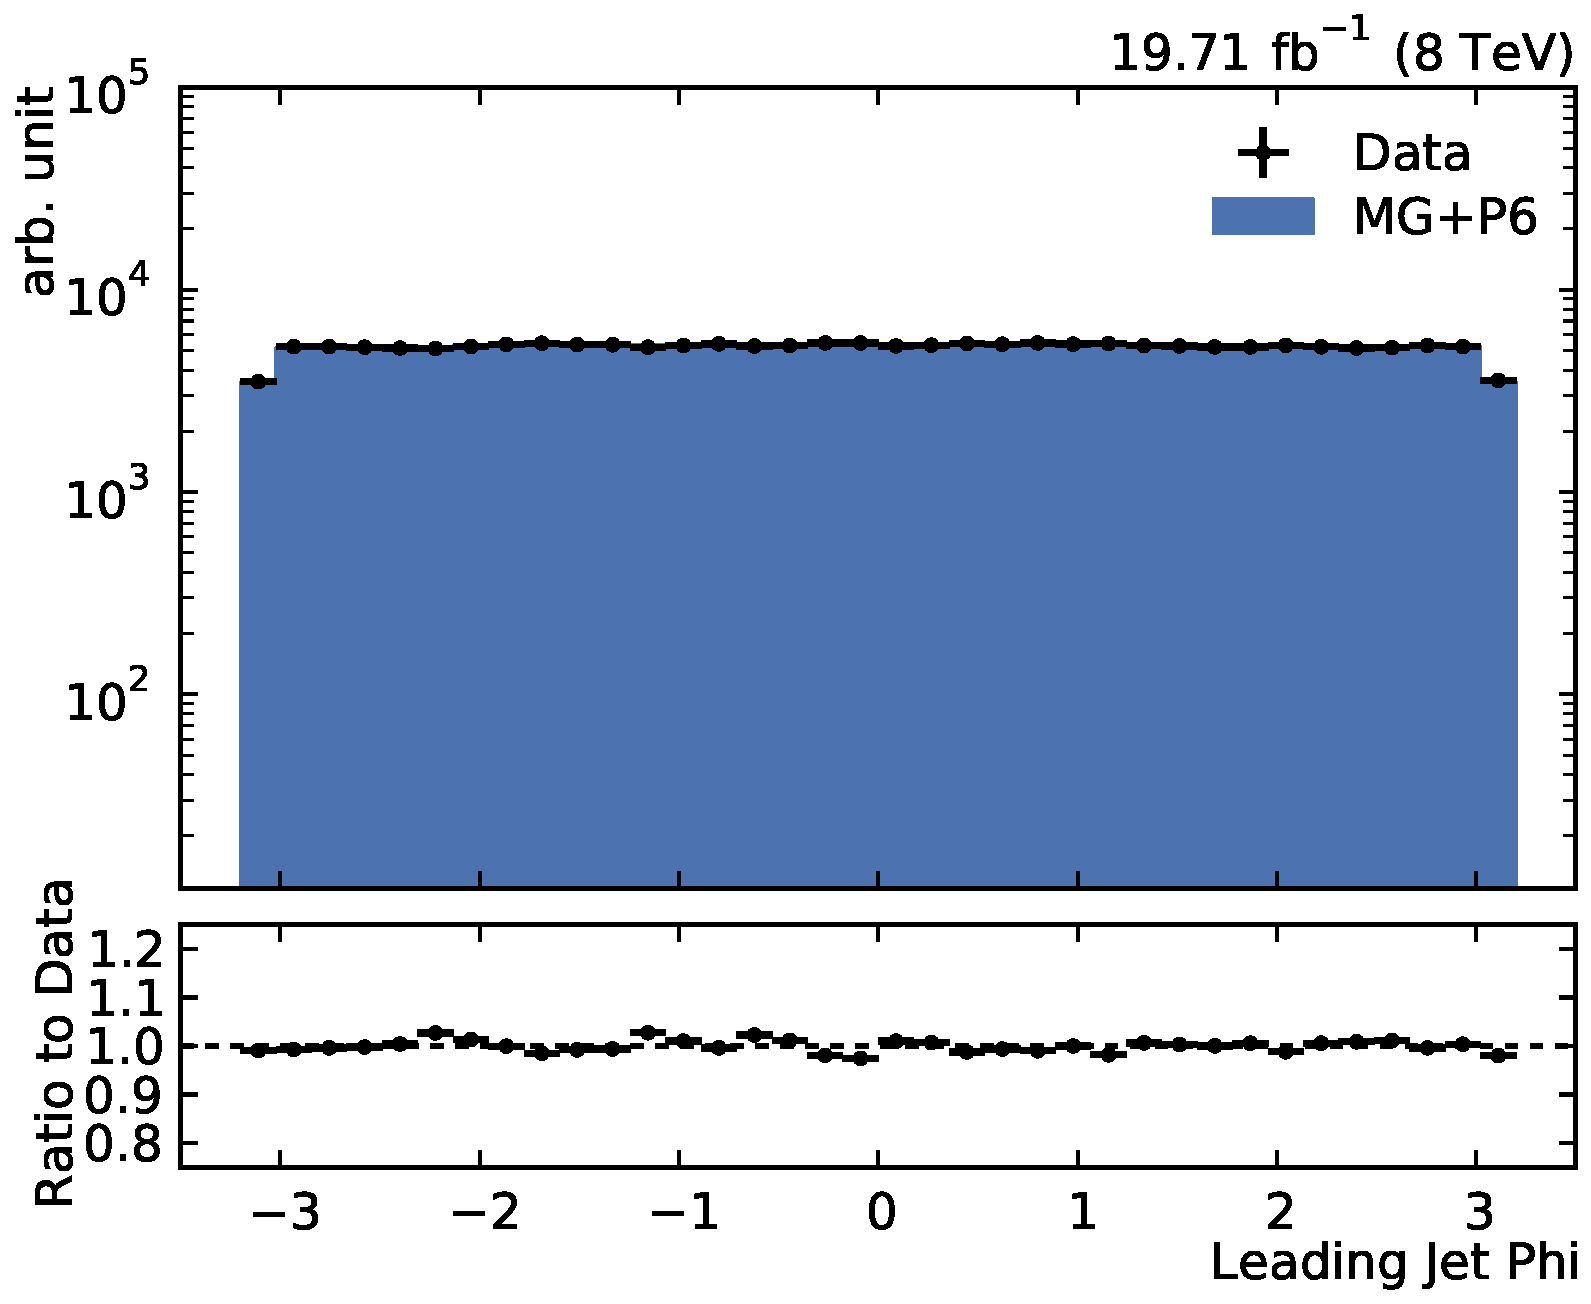
\includegraphics[width=0.45\textwidth]{figures/measurement/jet2phi_default.pdf}
    \caption[Control plots of kinematic quantities of the dijet system]{The plots show the basic kinematic quantities of the two leading jets in a selected event.
             The transvers momentum of the leading (left plot) and the second (right plots) jet is shown
         in the top row. The rapidity of the jets is shown in the middle row. The azimuthal angle of the
     leading jet and the second jet is shown on the bottom row.}
    \label{fig:controlplots:kinematic}
\end{figure}

\begin{figure}[htbp]
    \centering
    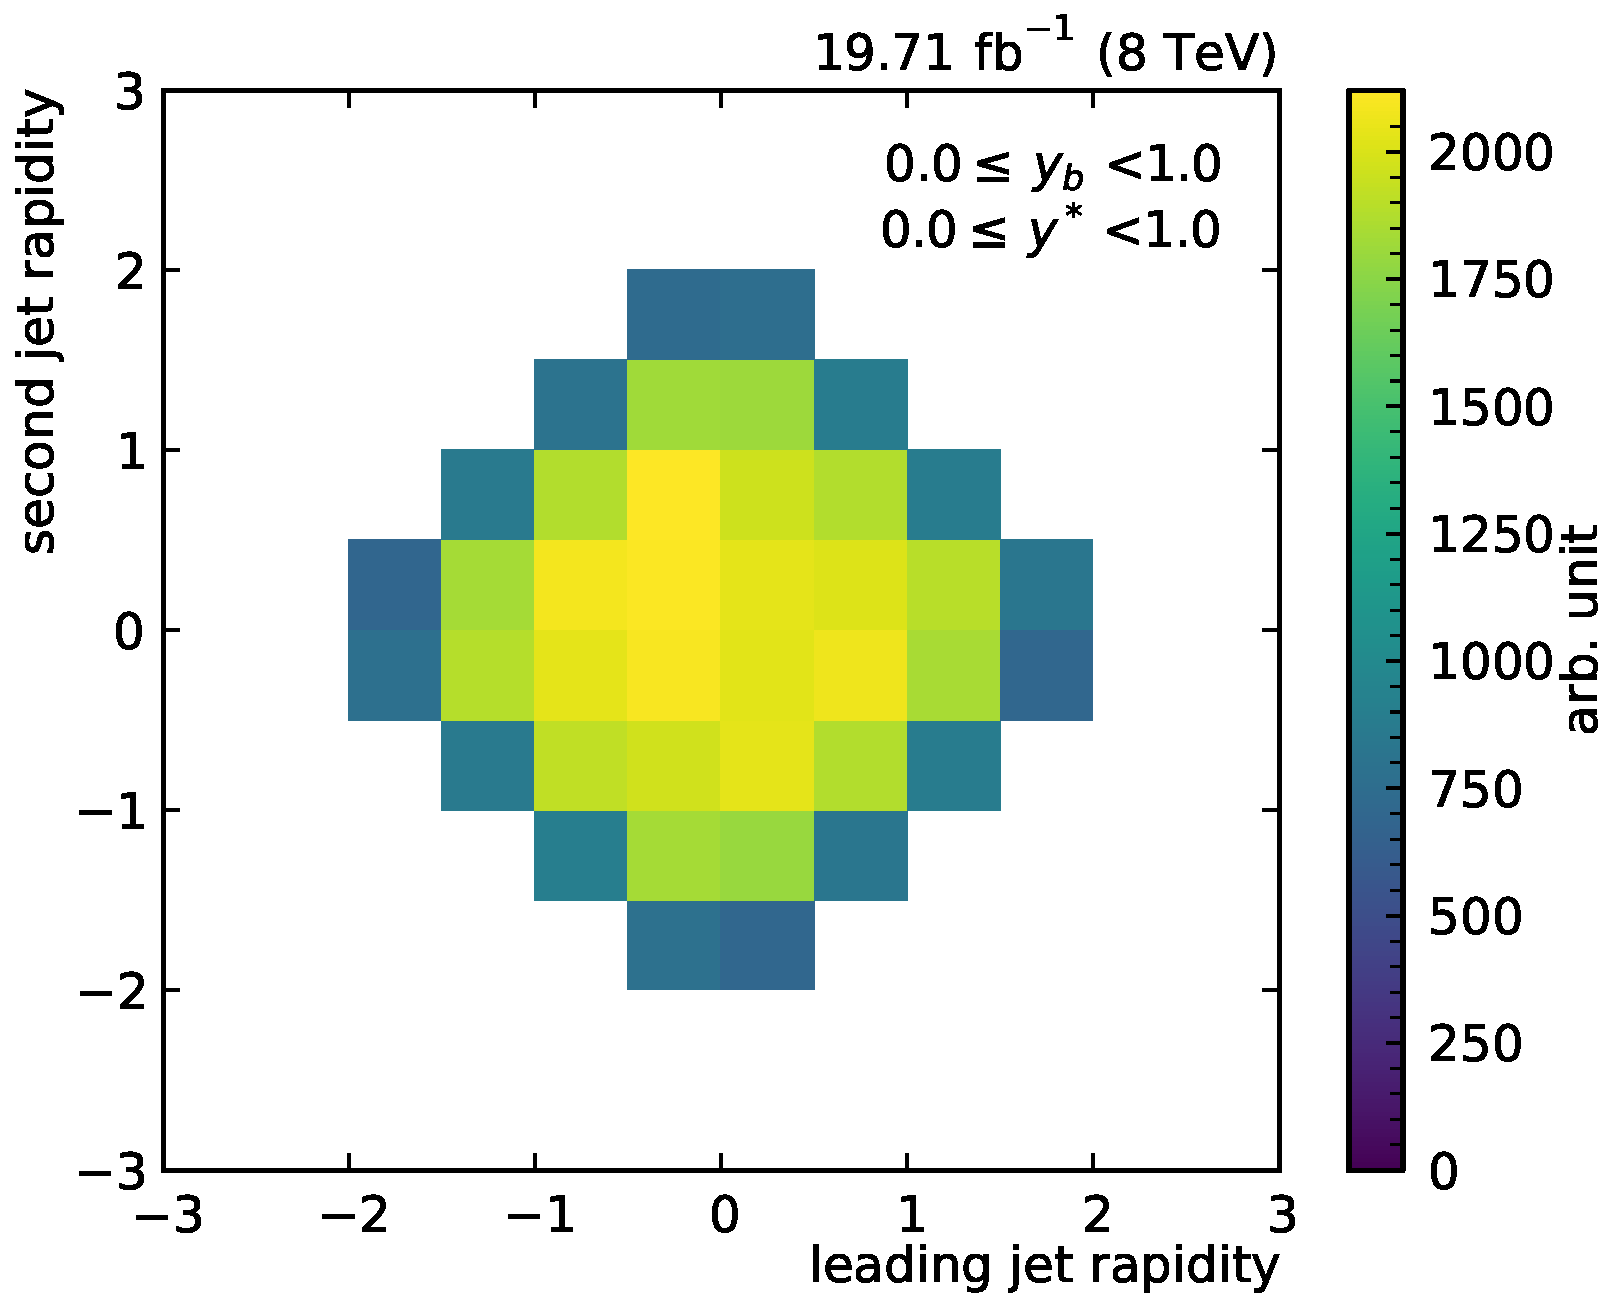
\includegraphics[width=0.45\textwidth]{figures/measurement/jet12_rapidity_yb0ys0.pdf}\hfill
    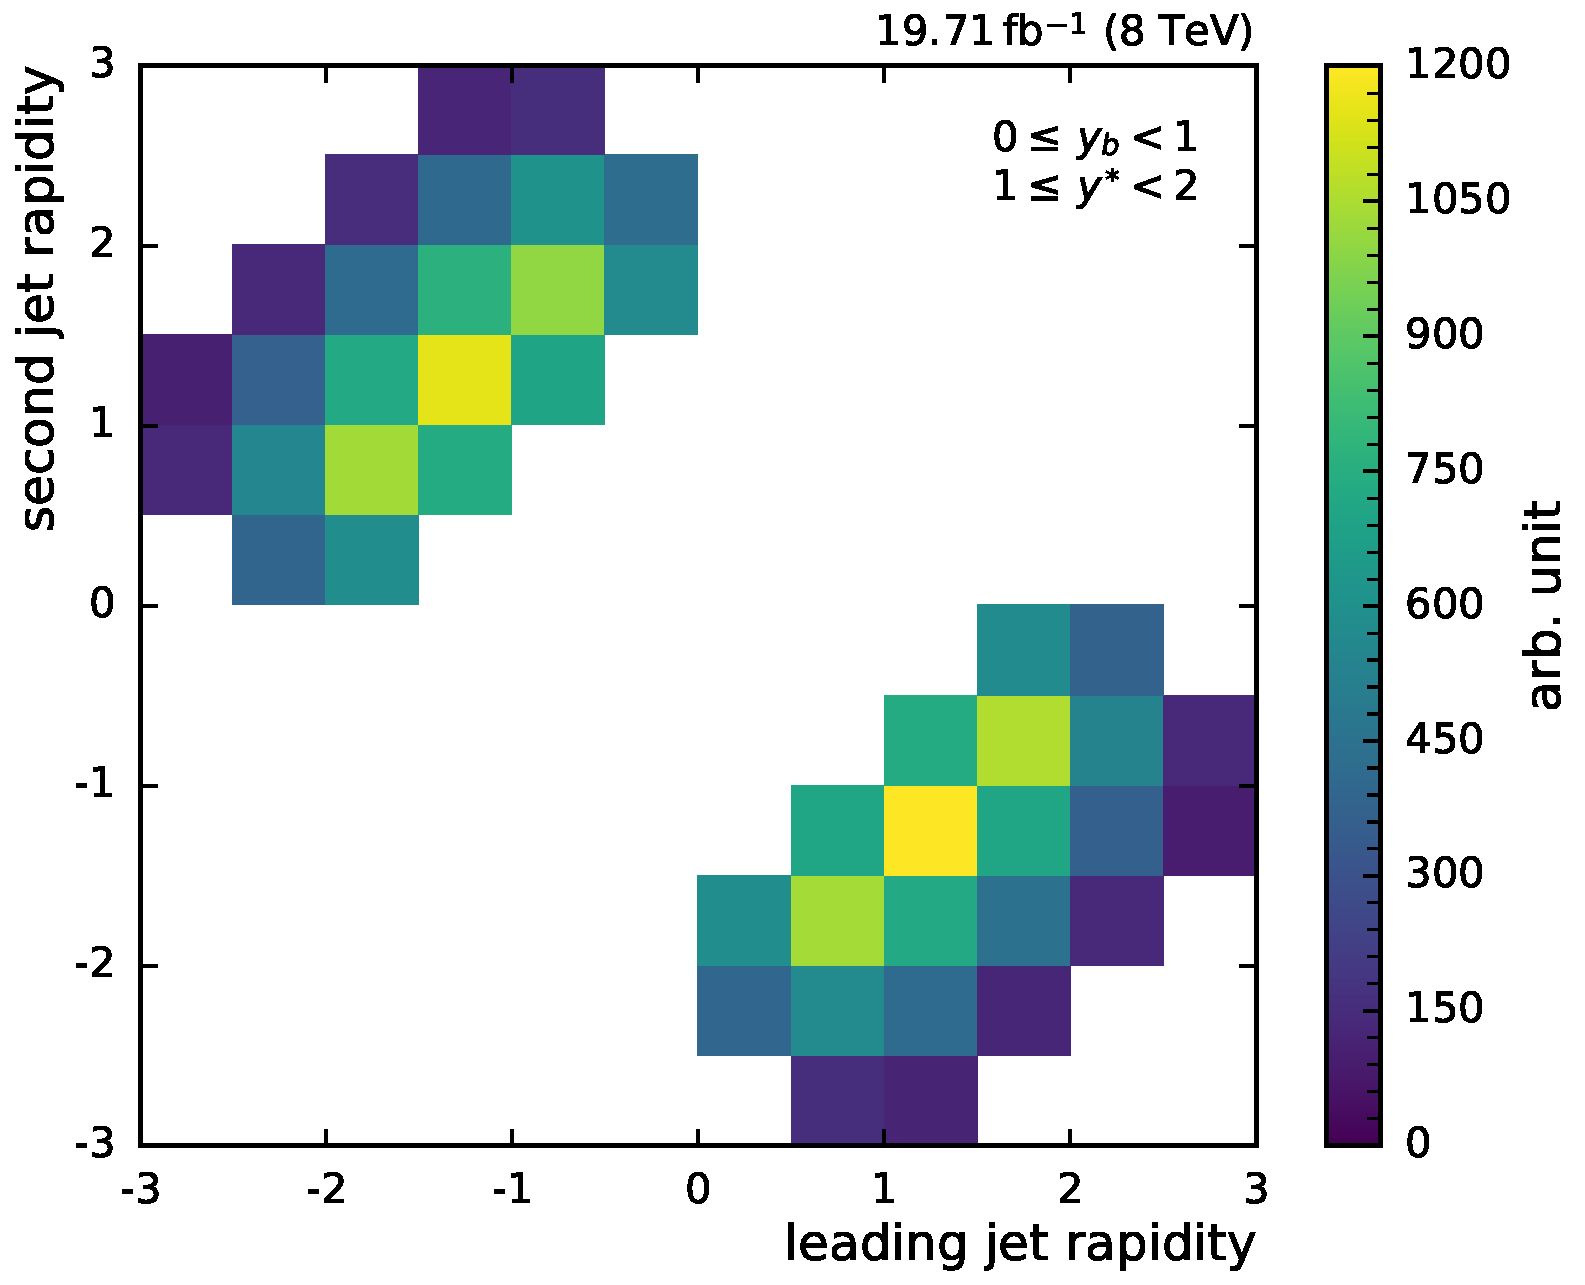
\includegraphics[width=0.45\textwidth]{figures/measurement/jet12_rapidity_yb0ys1.pdf}
    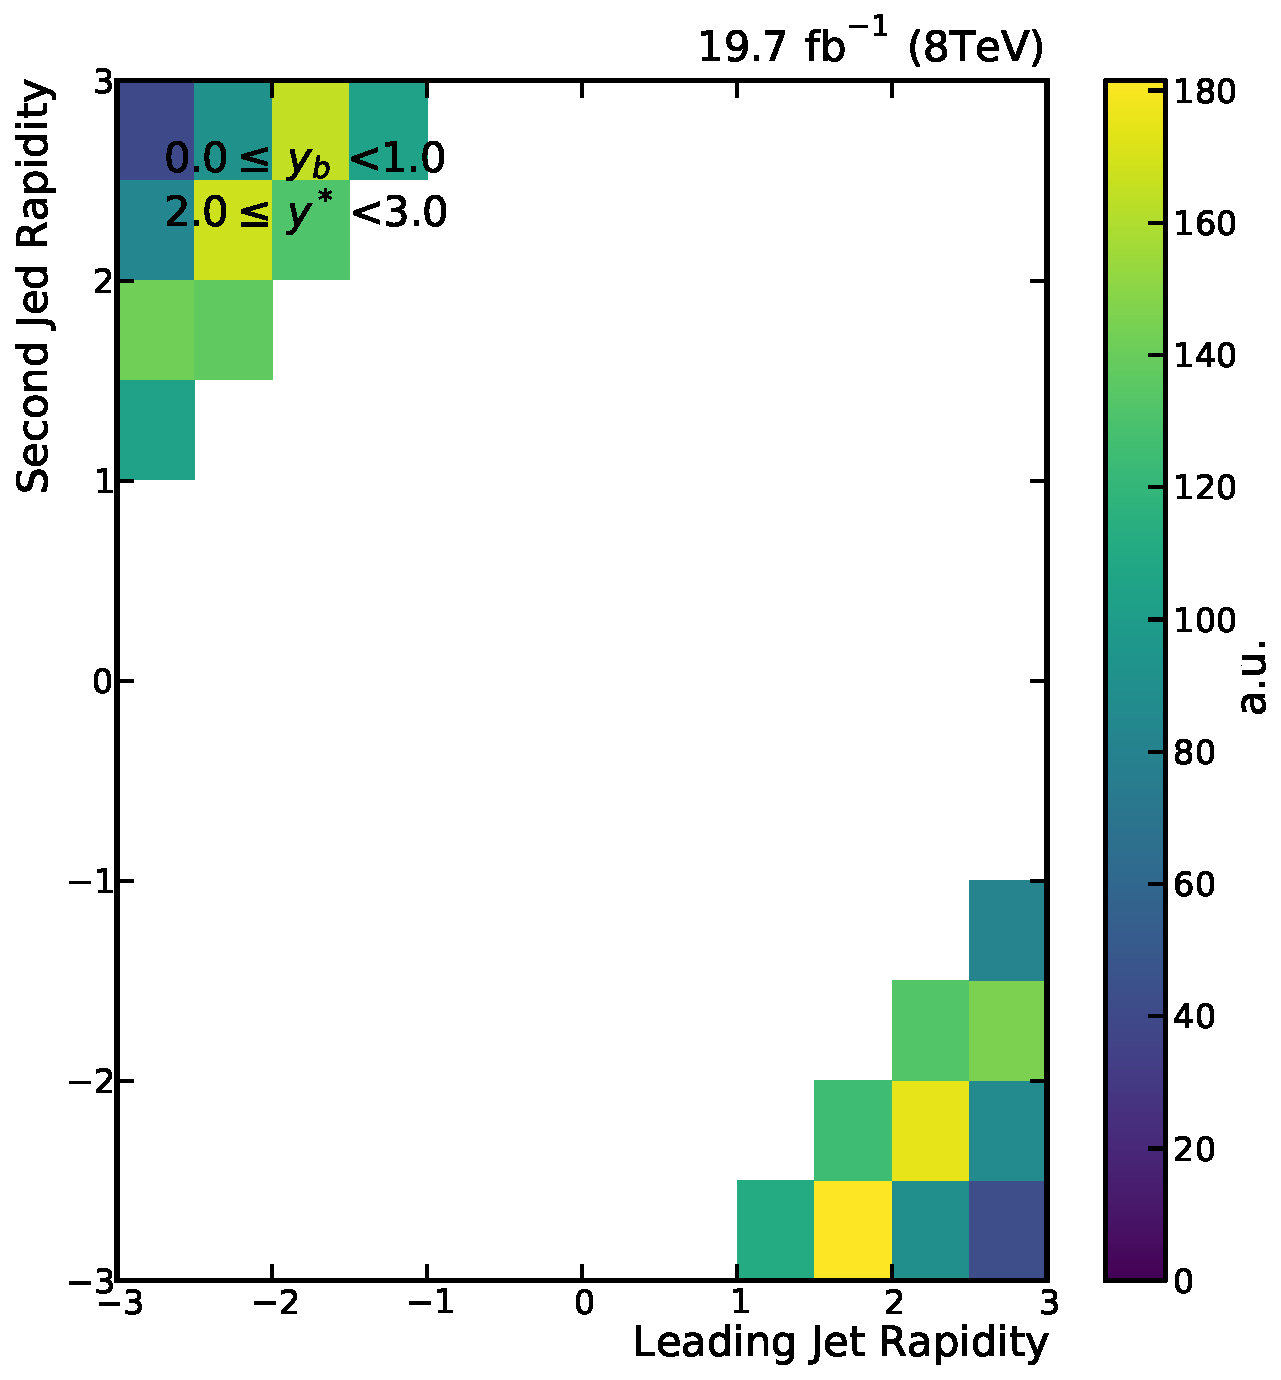
\includegraphics[width=0.45\textwidth]{figures/measurement/jet12_rapidity_yb0ys2.pdf}\hfill
    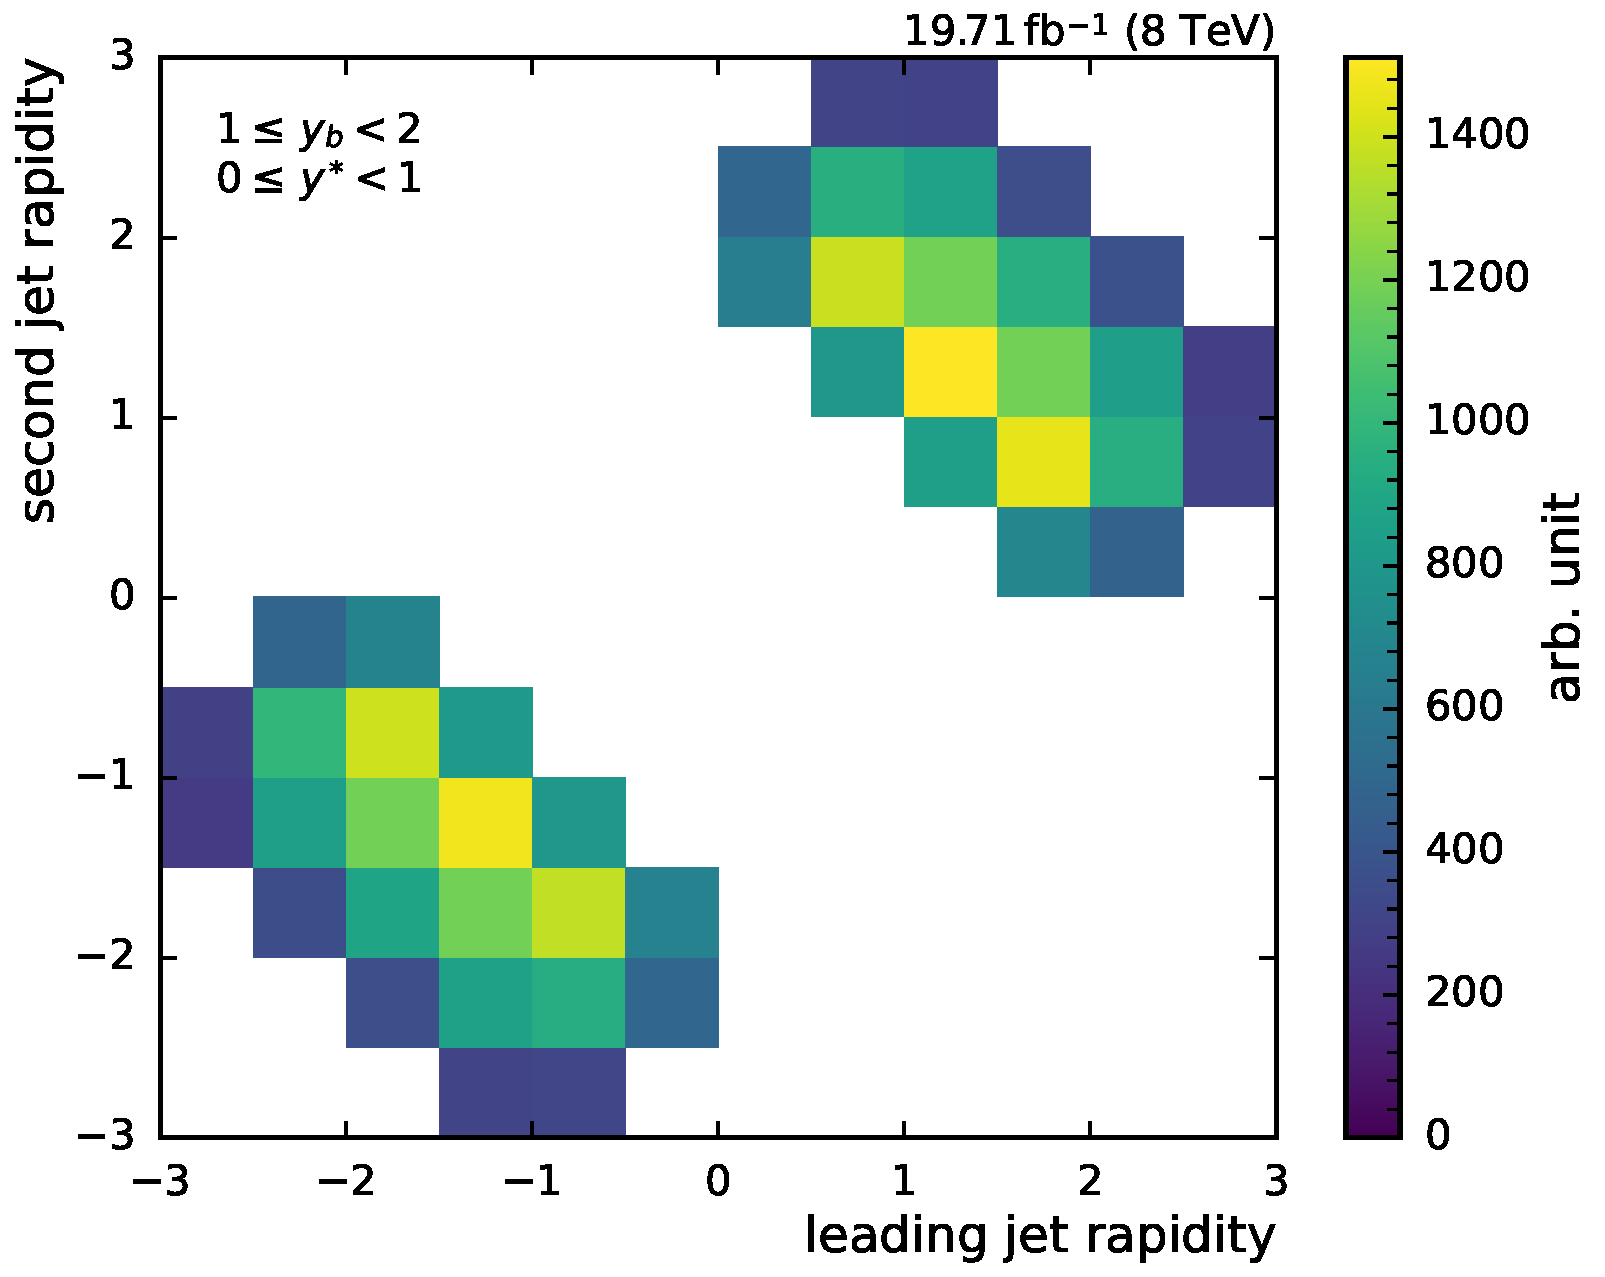
\includegraphics[width=0.45\textwidth]{figures/measurement/jet12_rapidity_yb1ys0.pdf}
    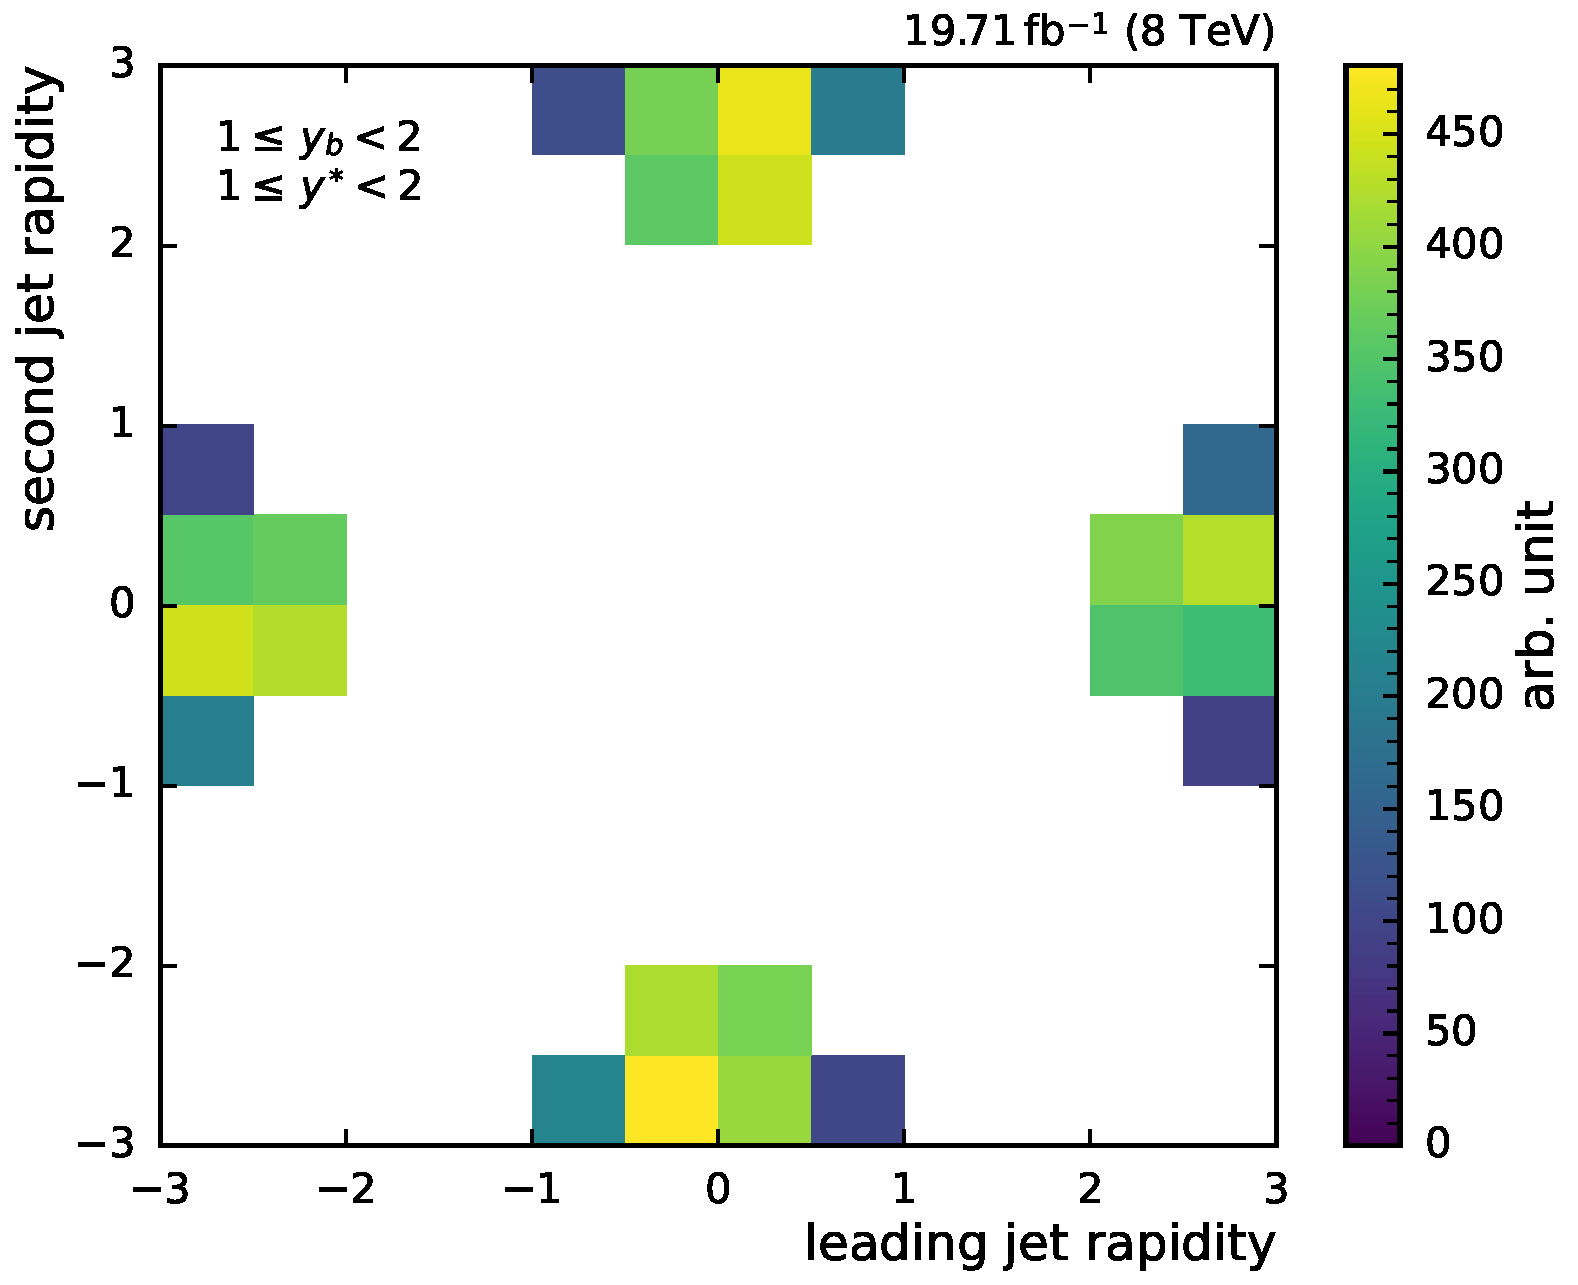
\includegraphics[width=0.45\textwidth]{figures/measurement/jet12_rapidity_yb1ys1.pdf}\hfill
    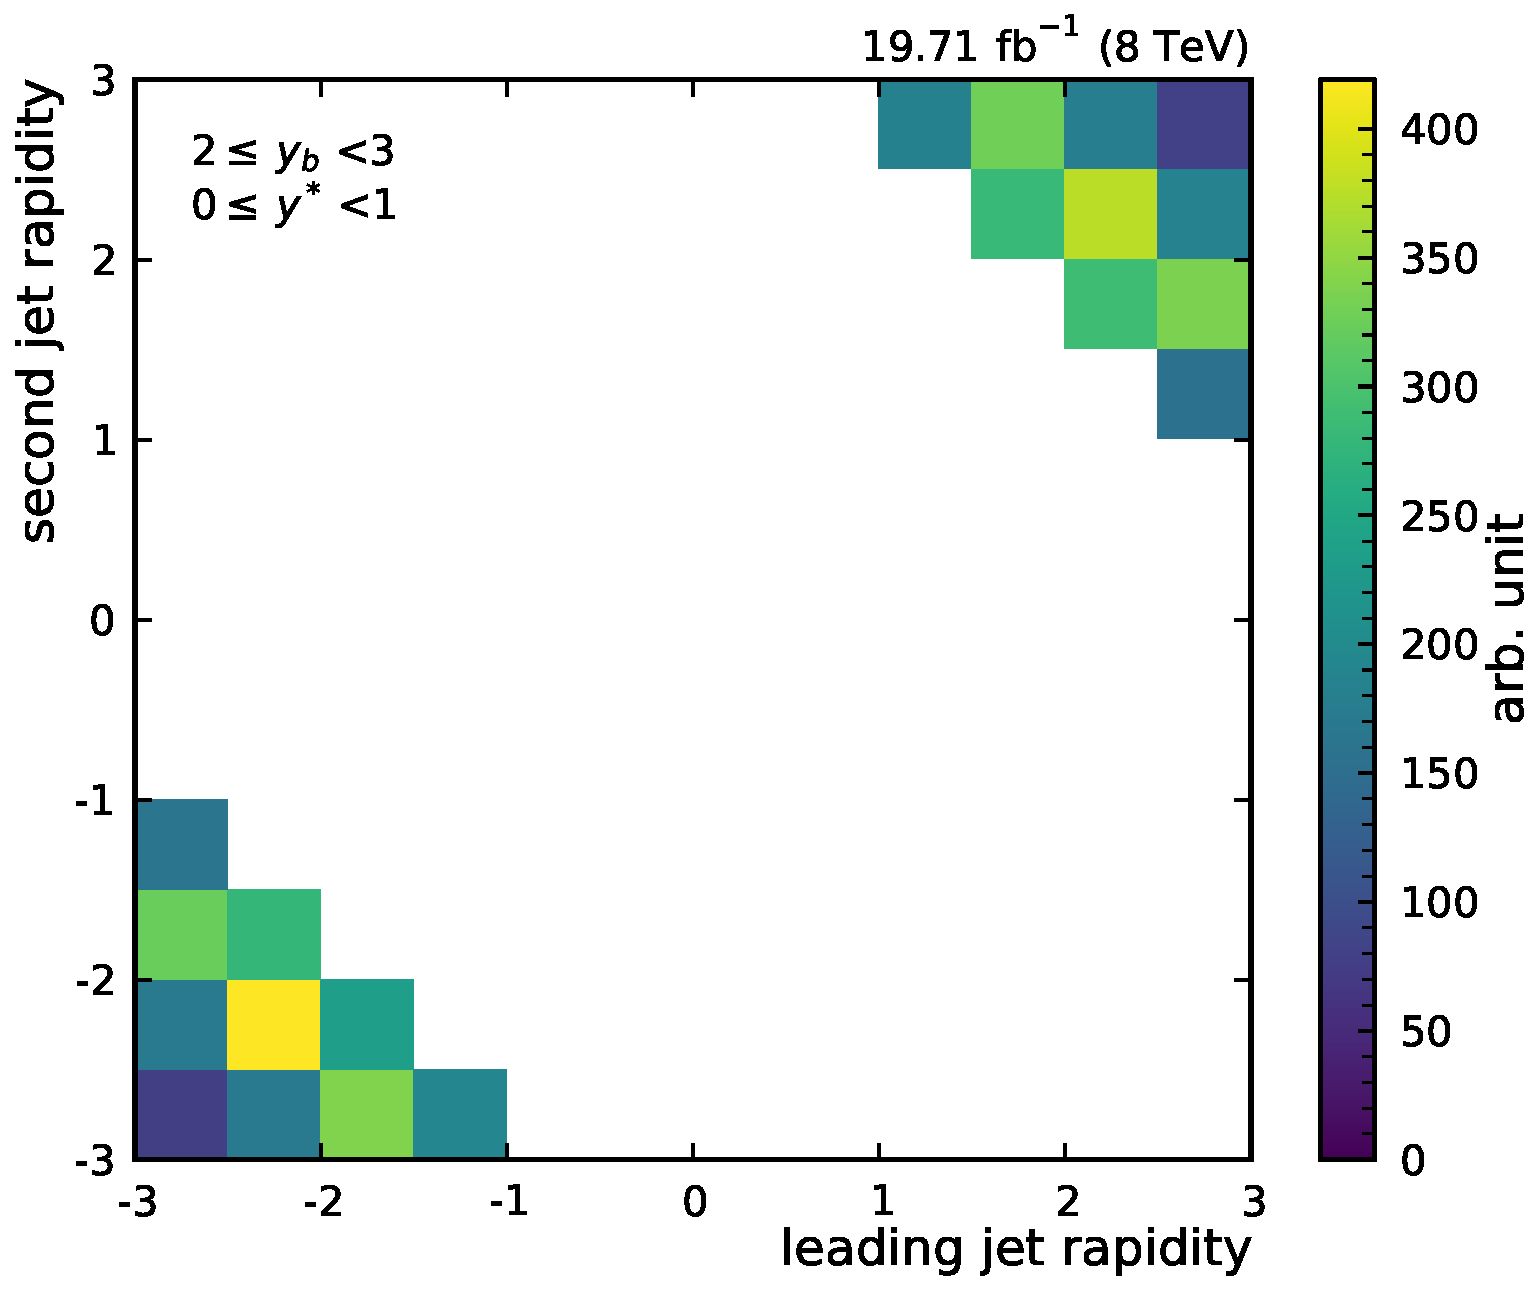
\includegraphics[width=0.45\textwidth]{figures/measurement/jet12_rapidity_yb2ys0.pdf}
    \caption[Rapidities of the two leading jets in the various \ystar and \yboost bins]{
        The plots show the basic kinematic quantities of the two leading jets in a selected event.
             The transvers momentum of the leading (left plot) and the second (right plots) jet is shown
         in the top row. The rapidity of the jets is shown in the middle row. The azimuthal angle of the
     leading jet and the second jet is shown on the bottom row.}
    \label{fig:controlplots:rapidity}
\end{figure}

\subsection{Cross section Comparison}

The Monte-Carlo simulation is used to compare the prediction including the detector simulation
to the measured data distribution which is smeared due to the finite detector resolution. Figure~\ref{fig:ratio_recotodata}
show the prediction of the MG+P6 and the P8 simulations as a ratio to the measured data spectrum.
While the agreement in the inner detector region is fine, the shape and especially the normalization
of the MC prediction cannot describe the data. Additionally the fixed order prediction of NLOJET++
is shown. This prediction is on parton level and is not corrected for non-perturbative effects. Still
it describes best the data apart from the known effects due to NP and detector resolution effects.

\begin{figure}[htbp]
    \centering
    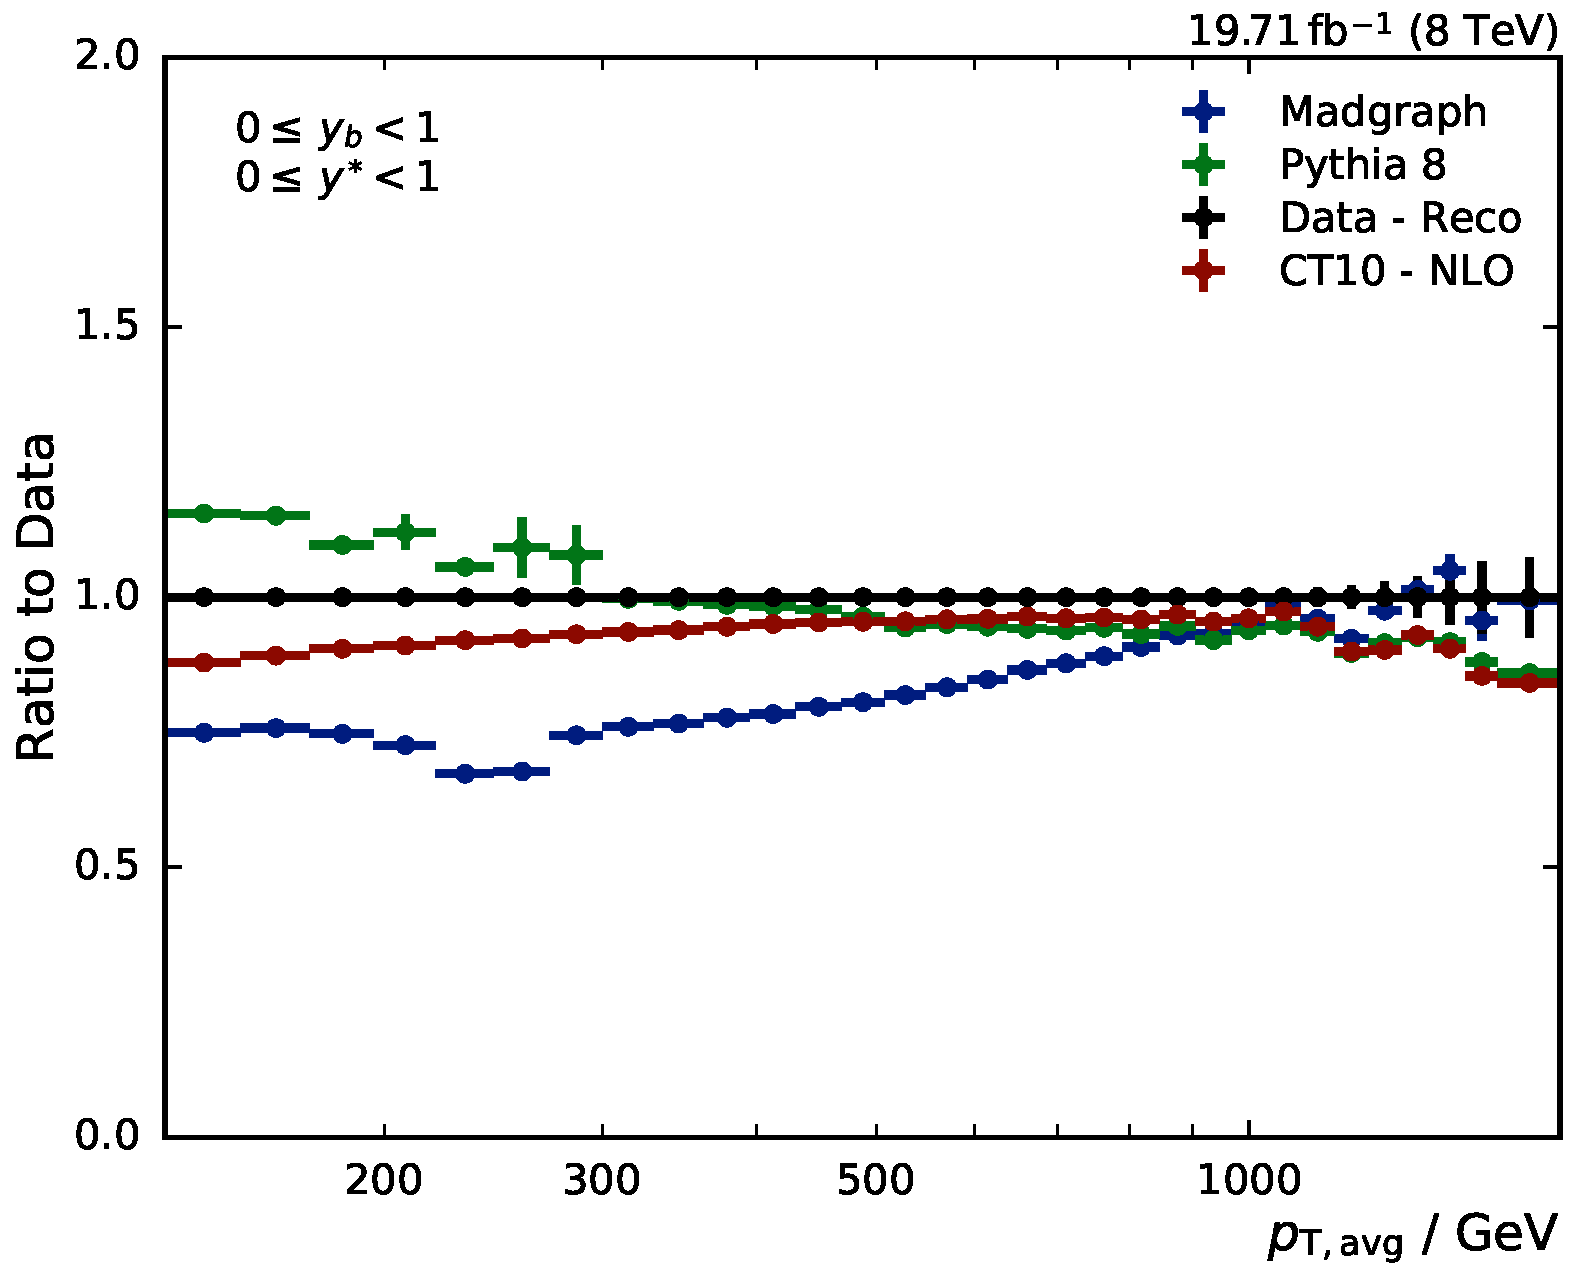
\includegraphics[width=0.45\textwidth]{figures/measurement/ratio_reco_to_data_yb0ys0.pdf}\hfill
    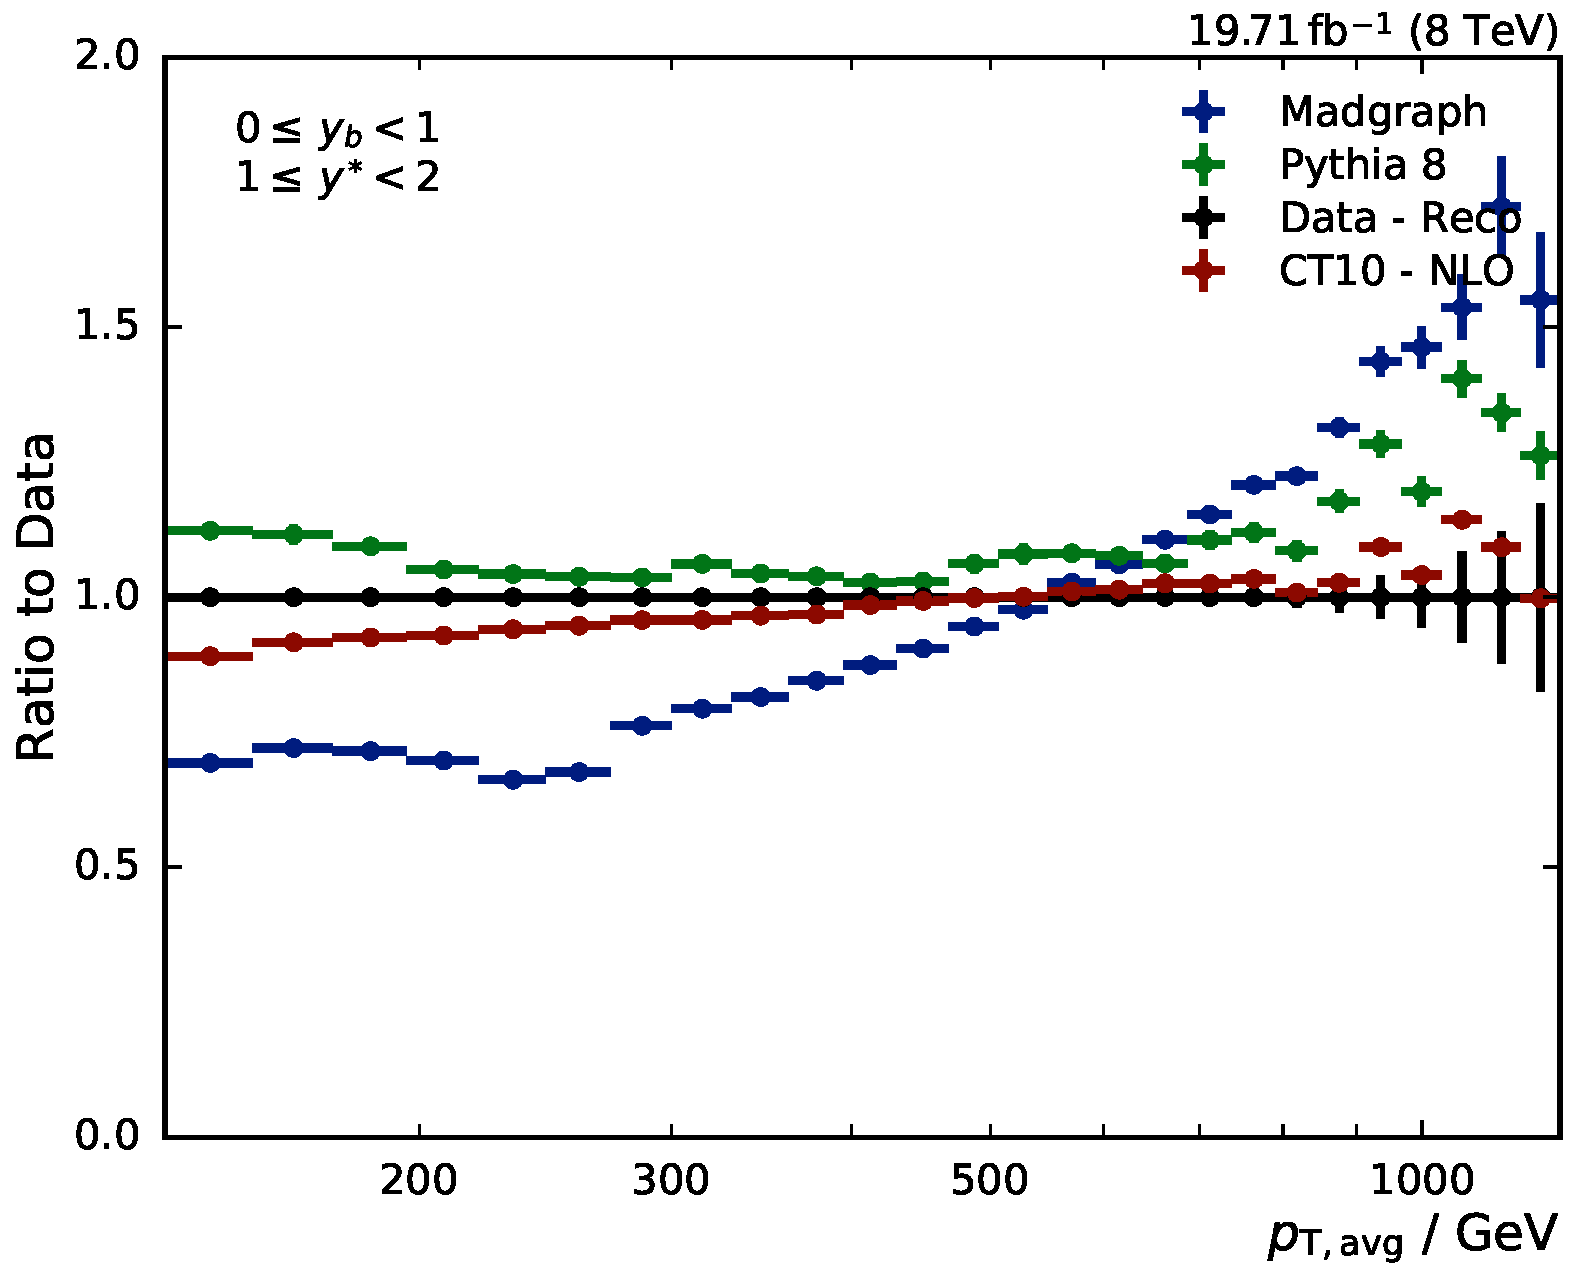
\includegraphics[width=0.45\textwidth]{figures/measurement/ratio_reco_to_data_yb0ys1.pdf}
    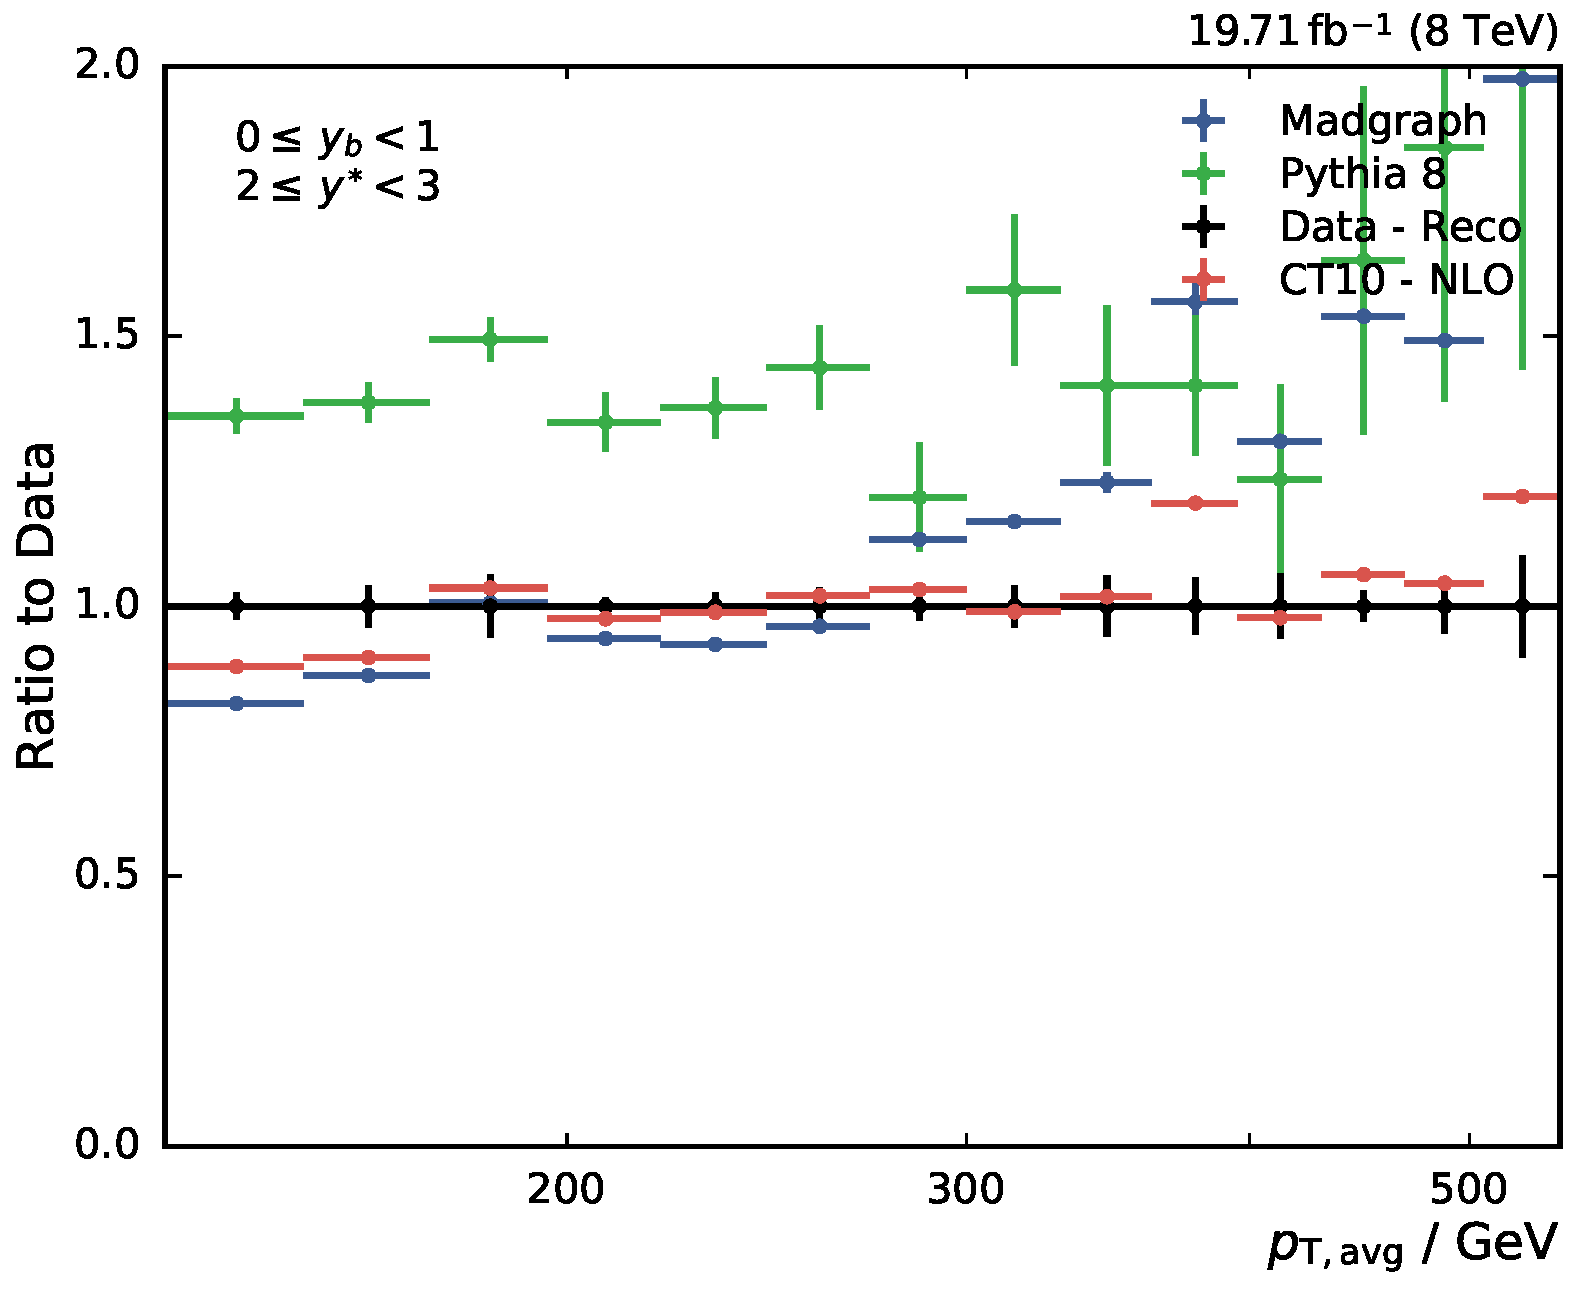
\includegraphics[width=0.45\textwidth]{figures/measurement/ratio_reco_to_data_yb0ys2.pdf}\hfill
    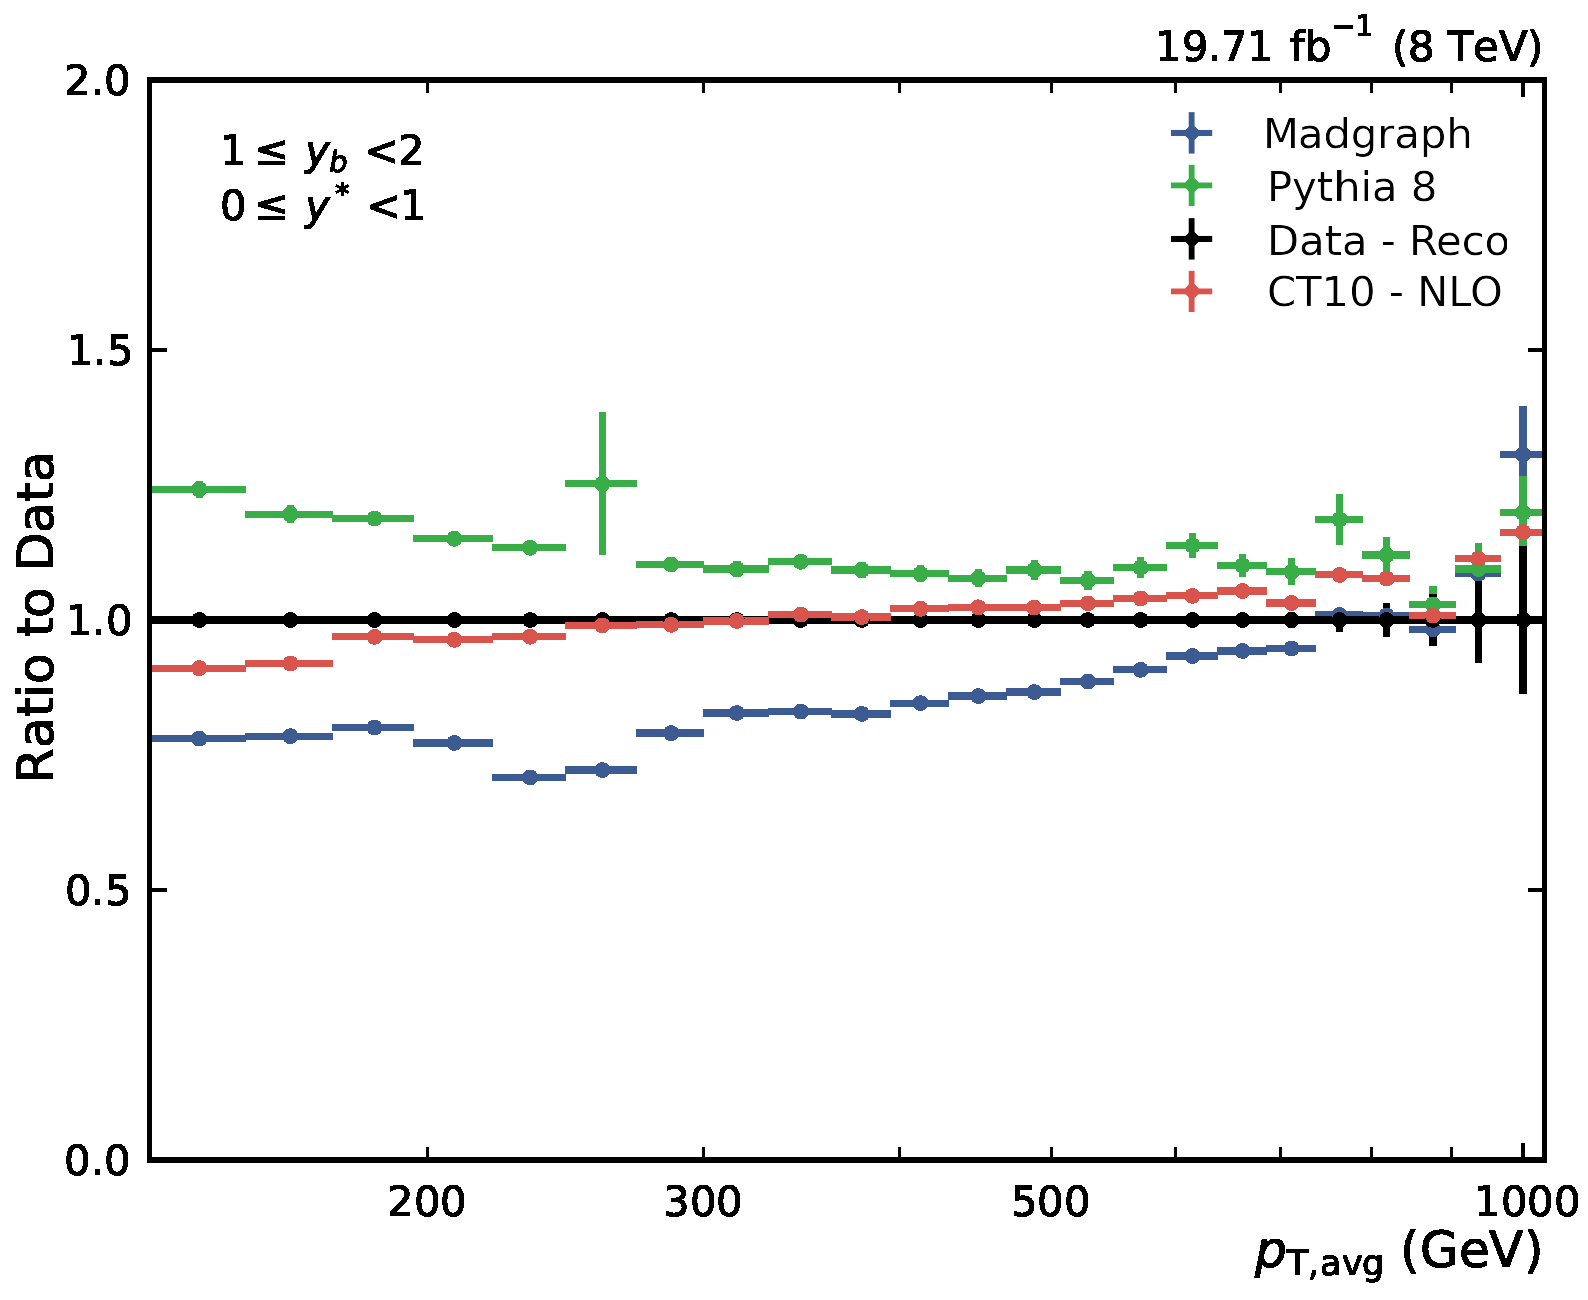
\includegraphics[width=0.45\textwidth]{figures/measurement/ratio_reco_to_data_yb1ys0.pdf}
    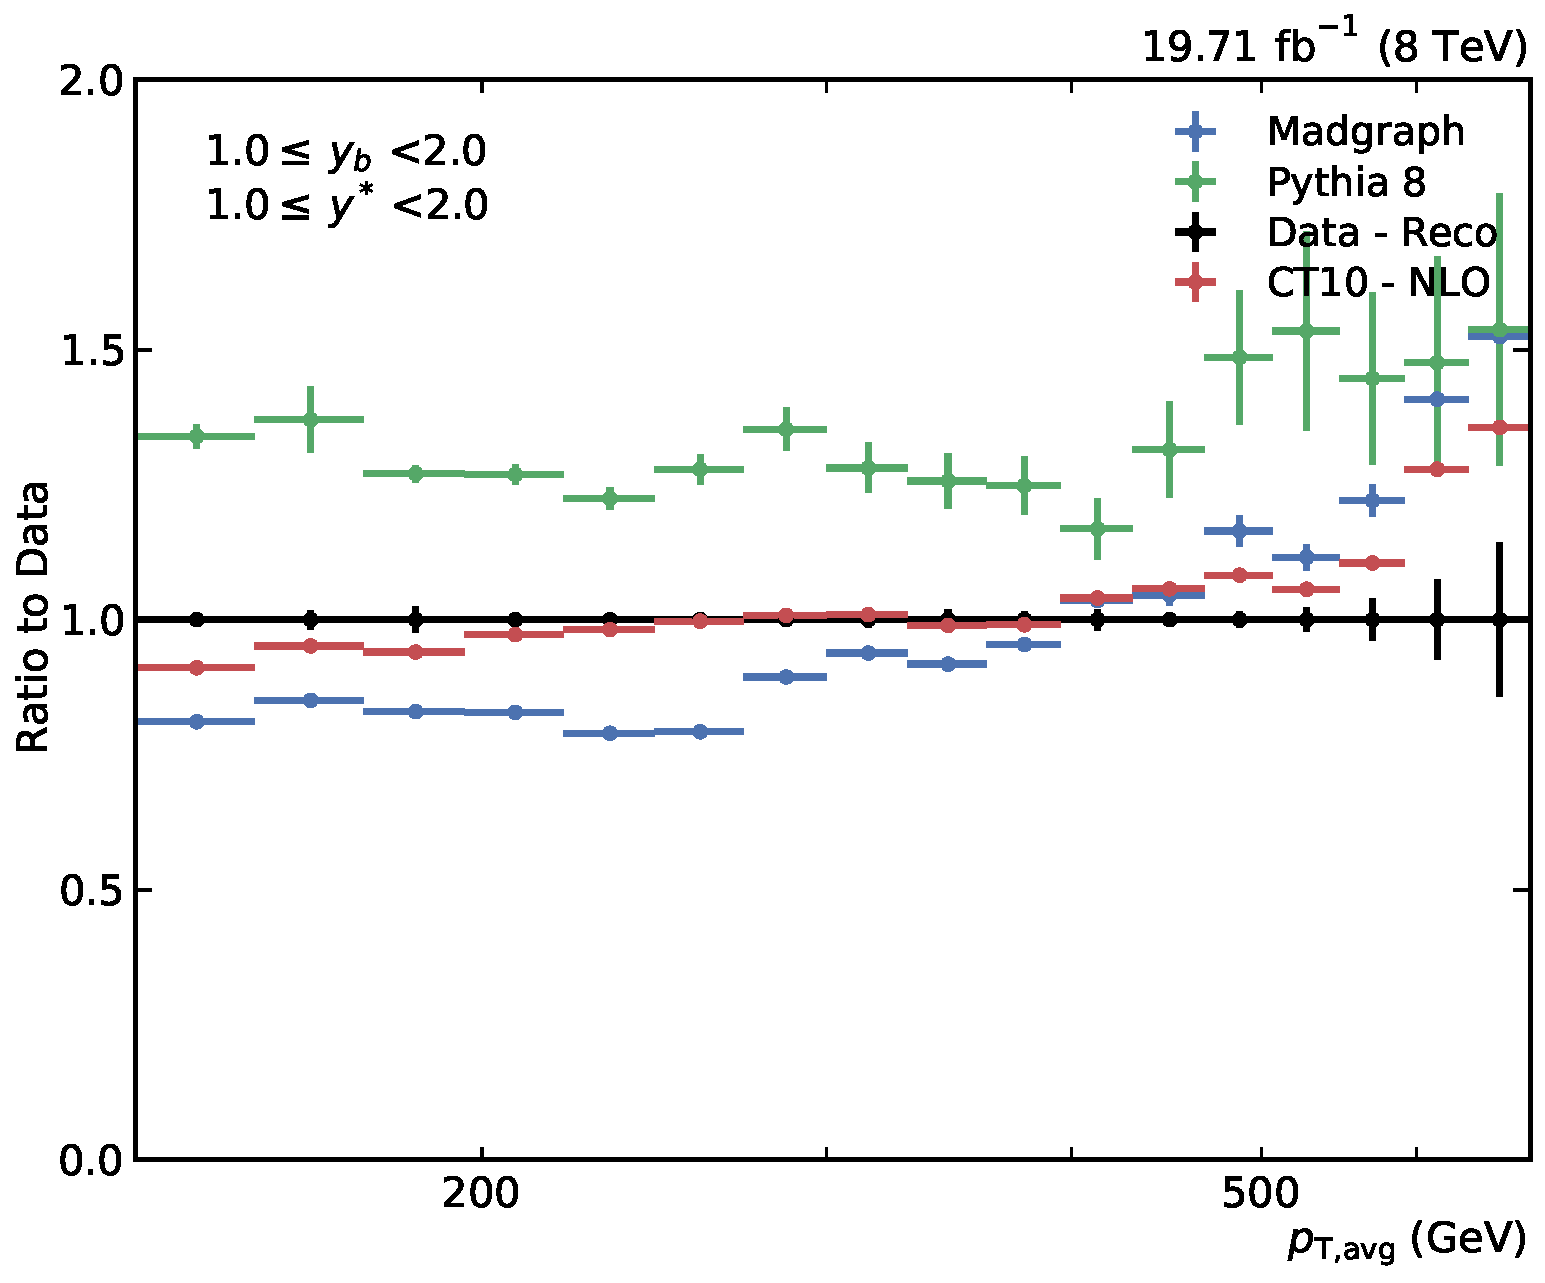
\includegraphics[width=0.45\textwidth]{figures/measurement/ratio_reco_to_data_yb1ys1.pdf}\hfill
    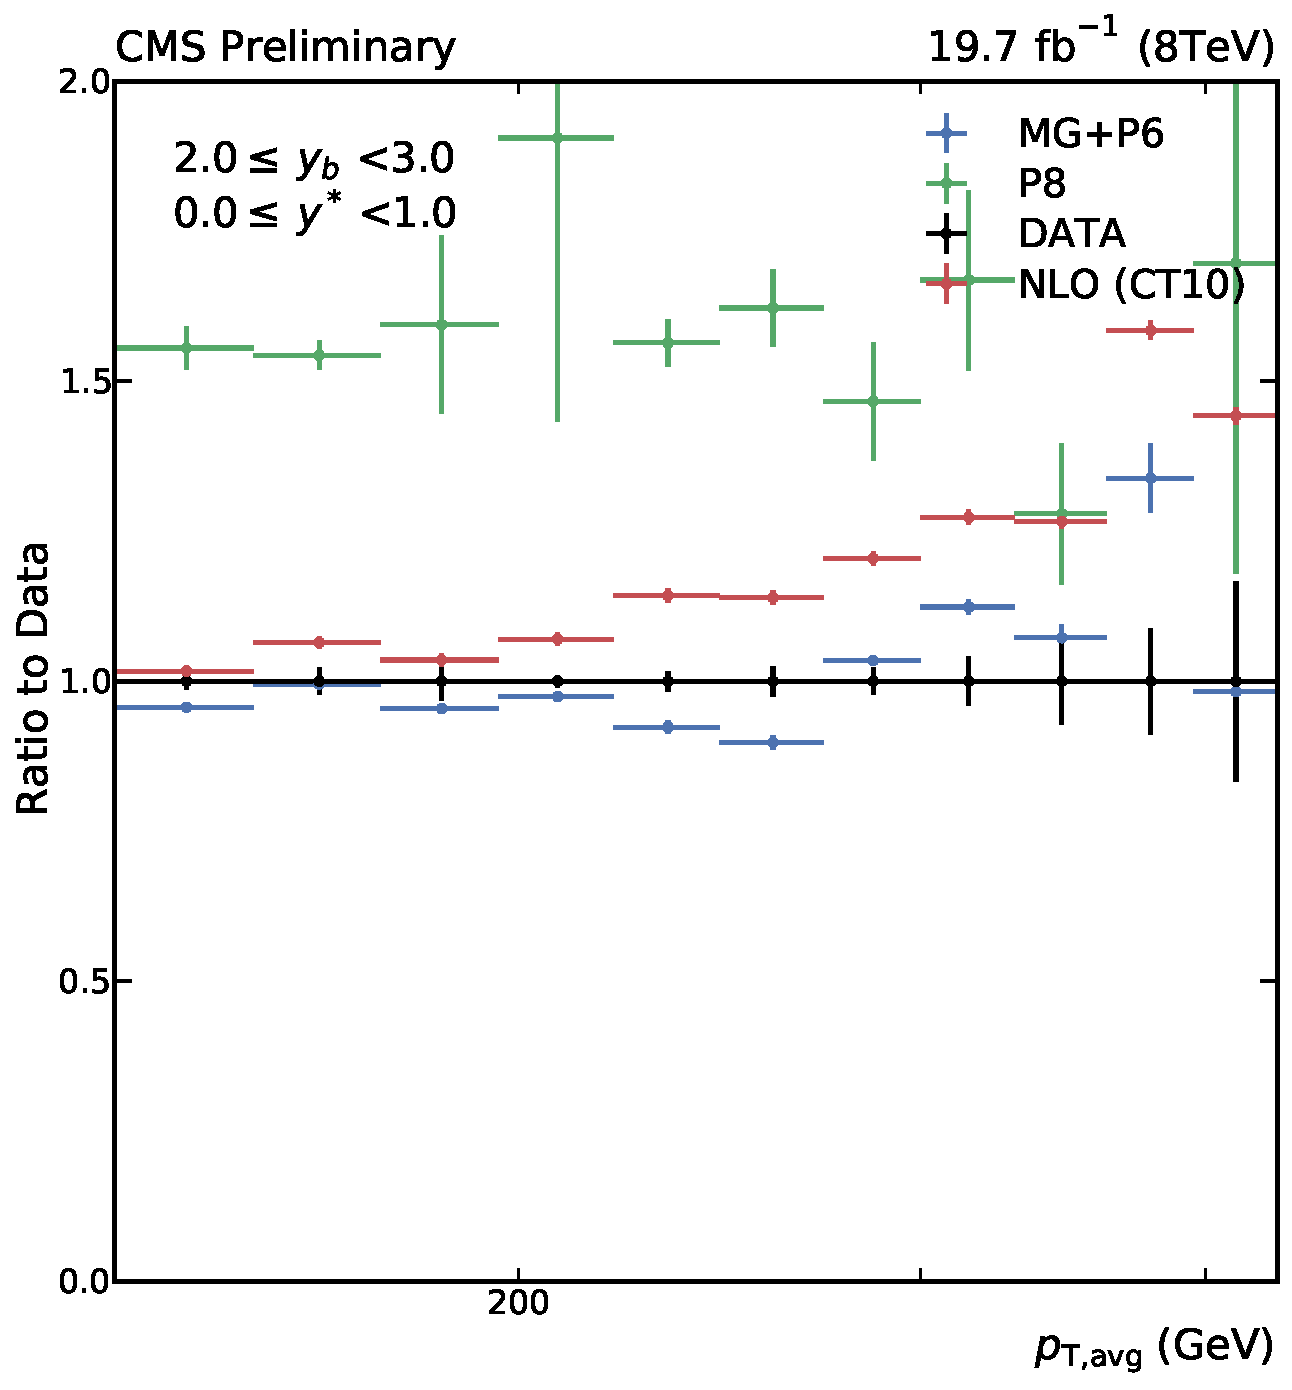
\includegraphics[width=0.45\textwidth]{figures/measurement/ratio_reco_to_data_yb2ys0.pdf}
    \caption[Comparison of data with simulated events]{Comparison of the measurement and the predictions using P8 and MG+P6. The data distributions are normalized
    to the integrated luminosity, the simulated events to the number of generated events and the cross section. The ratio of the simulated
    events to the data points is shown.}
    \label{fig:ratio_recotodata}
\end{figure}


\section{Dijet Transverse Momentum  Resolution}
\label{sec:resolution}

The true transverse momentum of the jets is smeared through the finite
resolution of the CMS detector. To measure the resolution of the \ptavg
observable, the truth information of Monte-Carlo events propagated through the
detector is used. The jets are clustered from stable generator particles as well
as from particle flow candidates reconstructed from the simulated detector
output. When studying the resolution, only events in which the leading two
generator jets are well matched to the reconstructed jets are used. The distance
$\Delta R$ in the $\eta$-$\phi$ plane is calculated as

\begin{equation}
\Delta R = \sqrt{\Delta \eta^2 + \Delta \phi^2}
\end{equation}
and needs to satisfy $\Delta R < 0.3$.

Measurements of the JERC working group at CMS show that the jet energy
resolution in data is actually worse than in simulation and the reconstructed
jet transverse momentum needs to be smeared additonally to match the resolution
in data. Table~\ref{tab:res_smearing} shows the smearing factors which need to
be applied on the transverse momentum of simulated reconstructed jets. The
smearing factors are derived separately for each region of the detector geometry.

\begin{table}[htbp]
\setlength\tabcolsep{4.5pt} 
    \centering
    \caption[Jet energy resolution scale factors]{
             The jet energy resolution in data is significantly worse than in
             simulated events. Therefore, the reconstructed jet tansverse
             momentum in simulated events is smeared using a factor $c$ to
             effectively match the resolution in data, following the
             recommendations of \JetMET group of CMS~\cite{jetmet:resolution}.
             The uncertainty on the resolution is given by an upwards and
             downwards variation $c_\mathrm{up}$ and
             $c_\mathrm{down}$ of the smearing factor.}
    \label{tab:res_smearing}

    \begin{tabular}{lccccccr}
    \toprule
    & & \multicolumn{6}{c}{$|\eta|$}\\\cmidrule{2-8}
               & $0.0$ -- $0.5$ & $0.5$ -- $1.1$ & $1.1$ -- $1.7$ & $1.7$ --
               $2.3$ & $2.3$ -- $2.8$ & $2.8$ -- $3.2$ & $3.2$ -- $5.0$\\
               $c_\text{res}$ &  &  &  & & & & \\\cmidrule{1-1}
    central    & 1.079                   & 1.099                   & 1.121    & 1.208                   & 1.254                   & 1.395    & 1.056\\
    down       & 1.053                   & 1.071                   & 1.092    & 1.162                   & 1.192                   & 1.332 & 0.865\\
    up         & 1.105                   & 1.127                   & 1.150 & 1.254                   & 1.316                   & 1.458 & 1.247\\
    \bottomrule
    \end{tabular}
\end{table}

Each reconstructed jet which is matched to a generated jet is smeared  using the formula
\begin{equation}
\ptreco = \max \left( 0, \ptgen + c(\eta) \cdot (\ptreco - \ptgen) \right)
\end{equation}

After applying the mentioned correction factor, the average dijet
transverse momentum is calculated both using the generator particle jets and
the particle flow jets on detector level. The response $R$ is calculated as

\begin{equation}
    R = \frac{\ptavg^{\text{reco}}}{\ptavg^{\text{gen}}}
\end{equation}

Since the response is dependent on the detector region as well as the transverse
momentum of the jets, the dijet average transverse momentum resolution is
calculated as a function of \ptavggen for each measurement bin in the phase
space variables \ystar and \yboost. Figure~\ref{fig:gen_vs_reco_over_gen} shows the
two-dimensional distributions for each bin.

\begin{figure}[htbp]
    \centering
    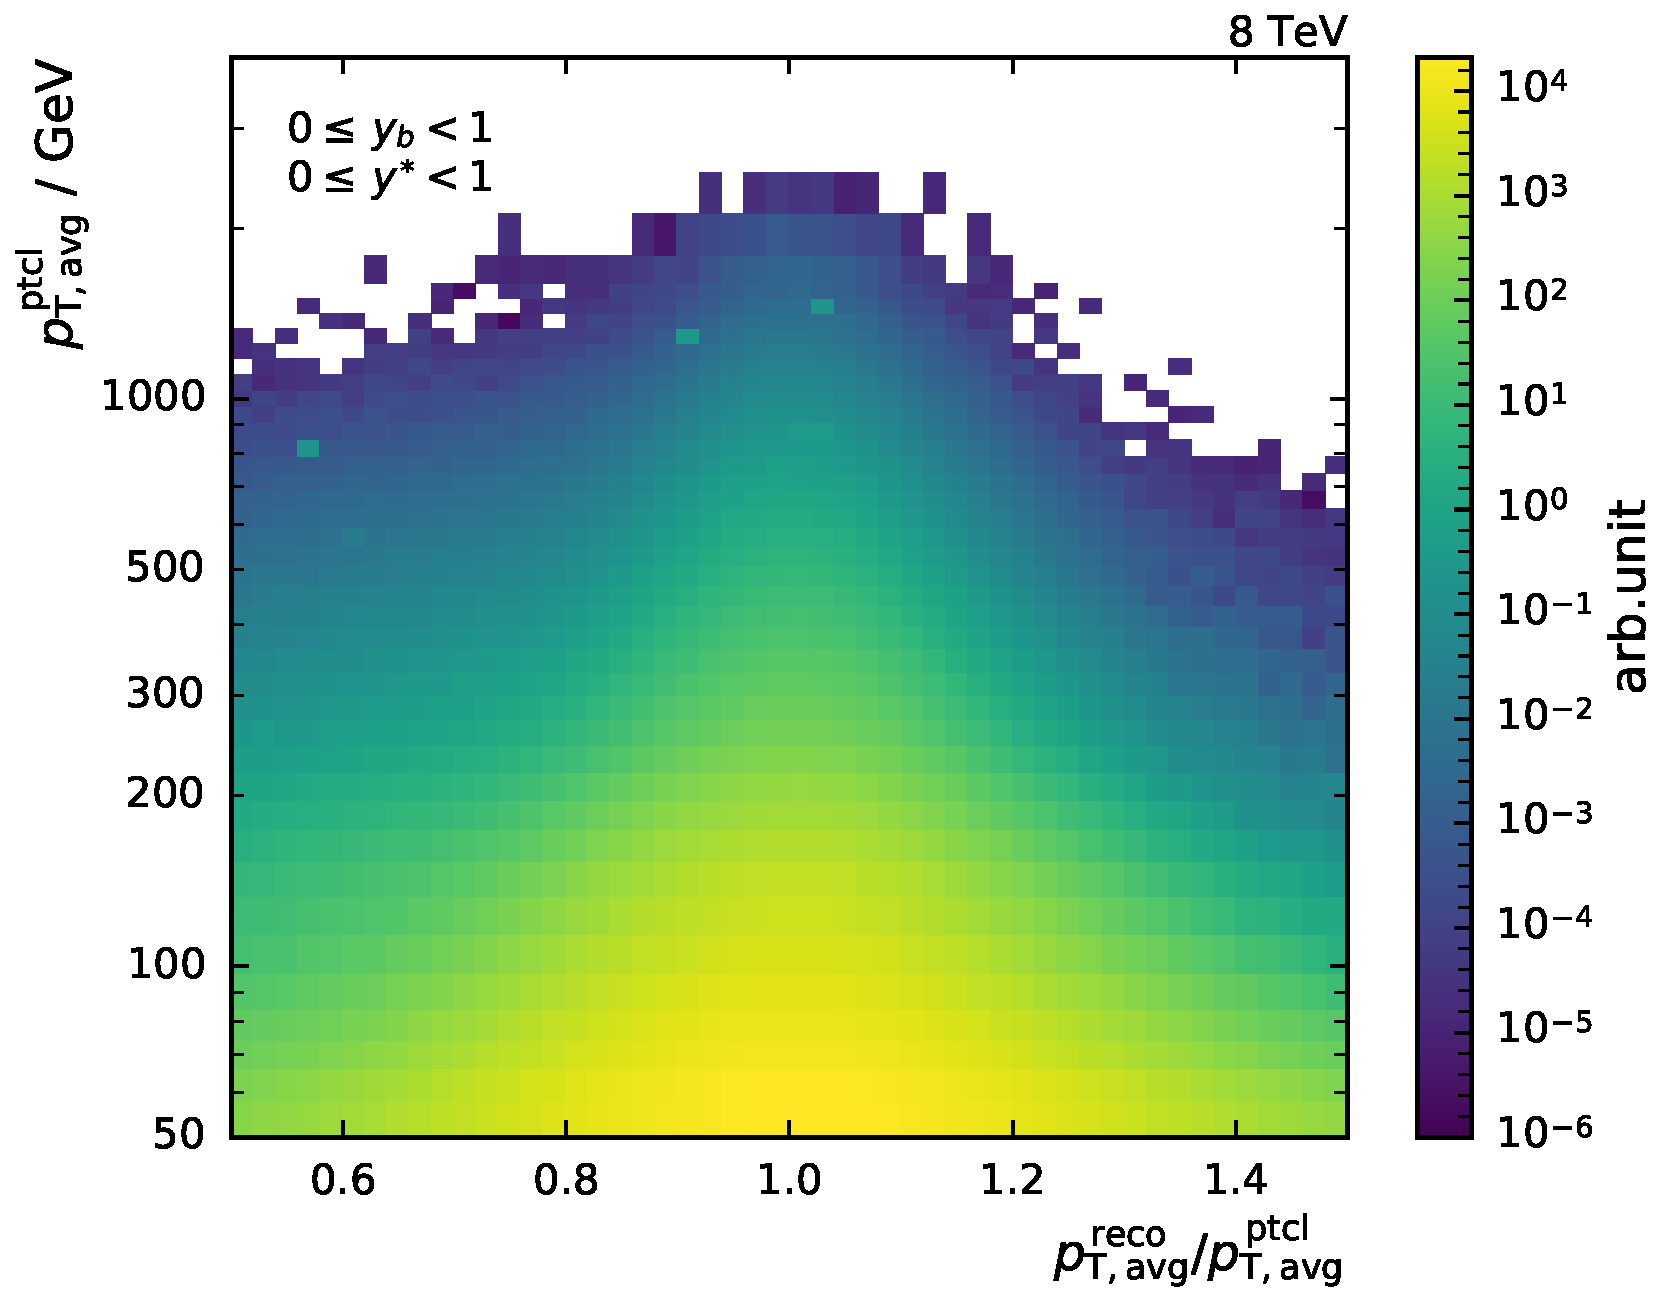
\includegraphics[width=0.45\textwidth]{figures/measurement/gen_vs_reco_vs_gen_ptavg_yb0ys0.pdf}\hfill
    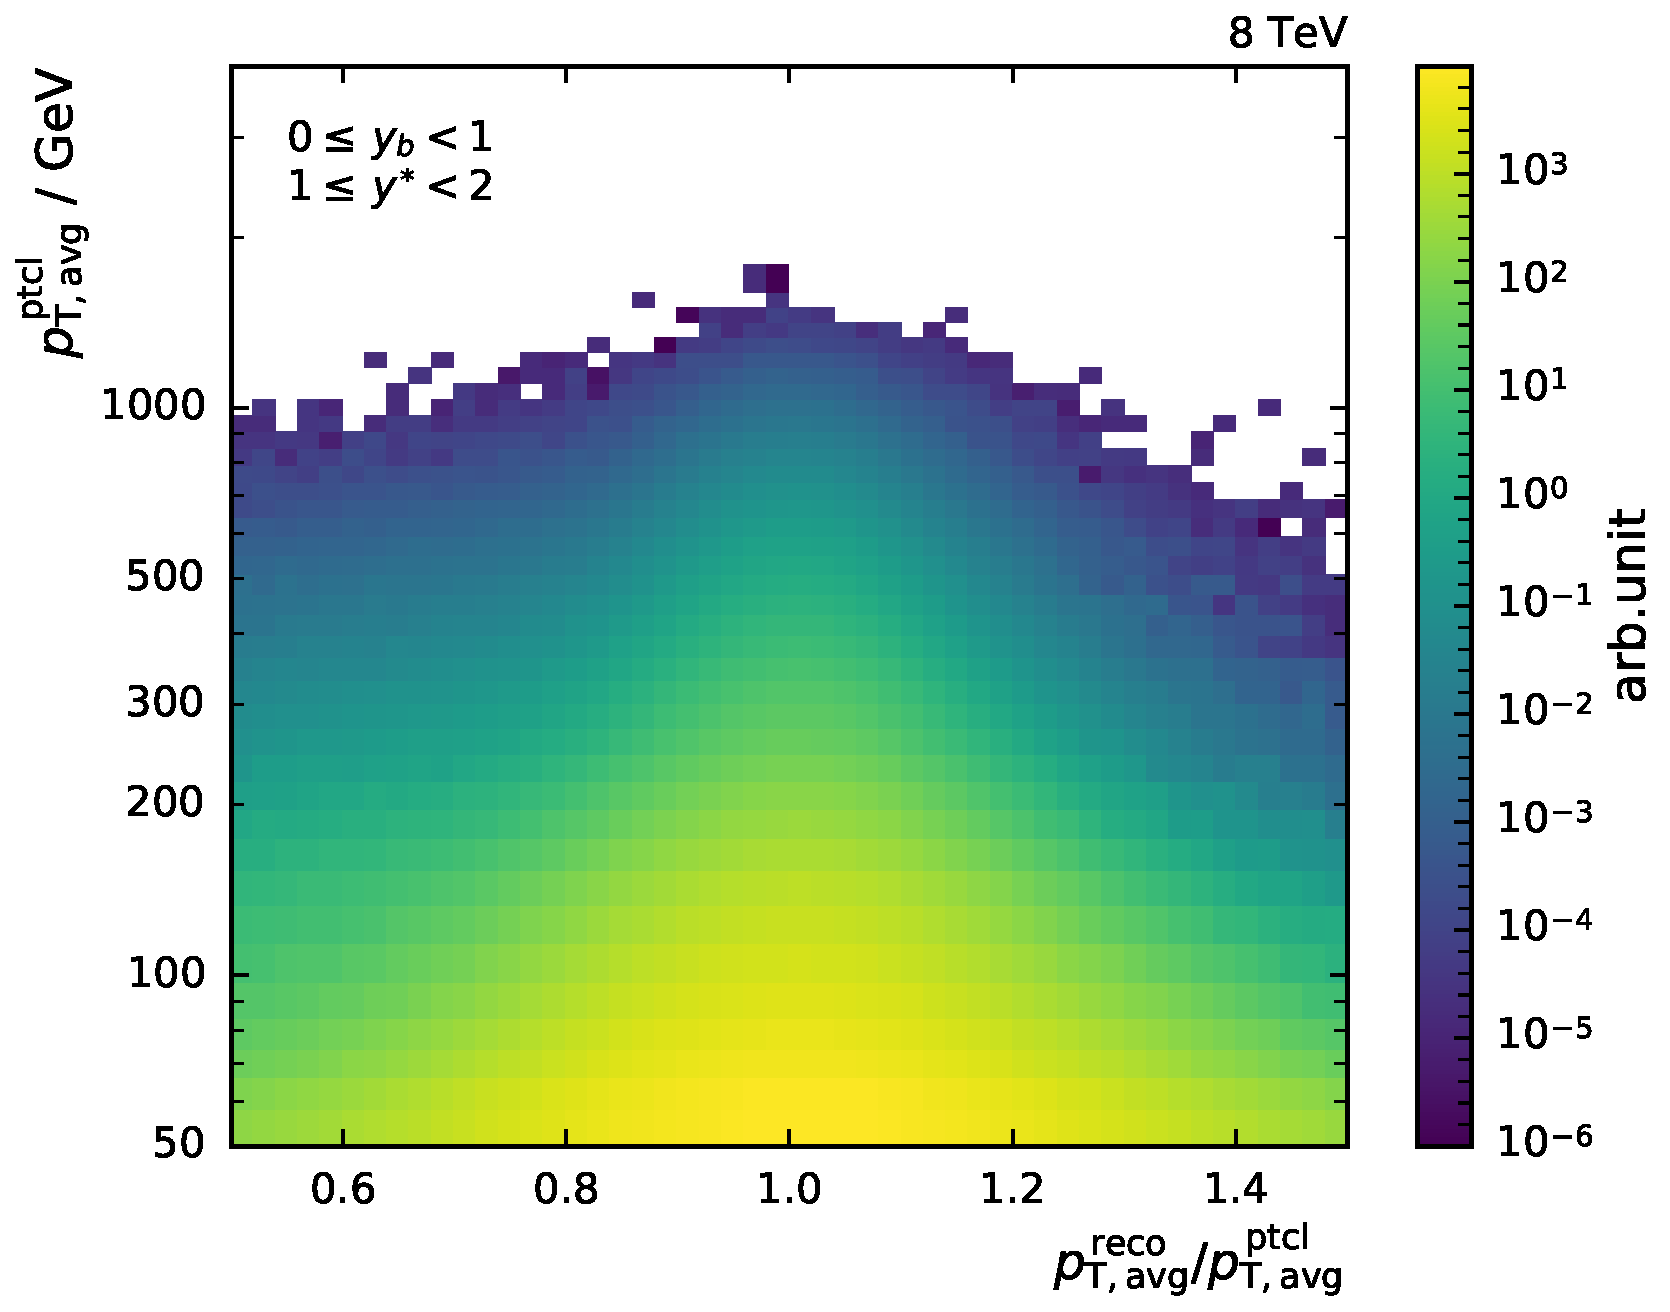
\includegraphics[width=0.45\textwidth]{figures/measurement/gen_vs_reco_vs_gen_ptavg_yb0ys1.pdf}
    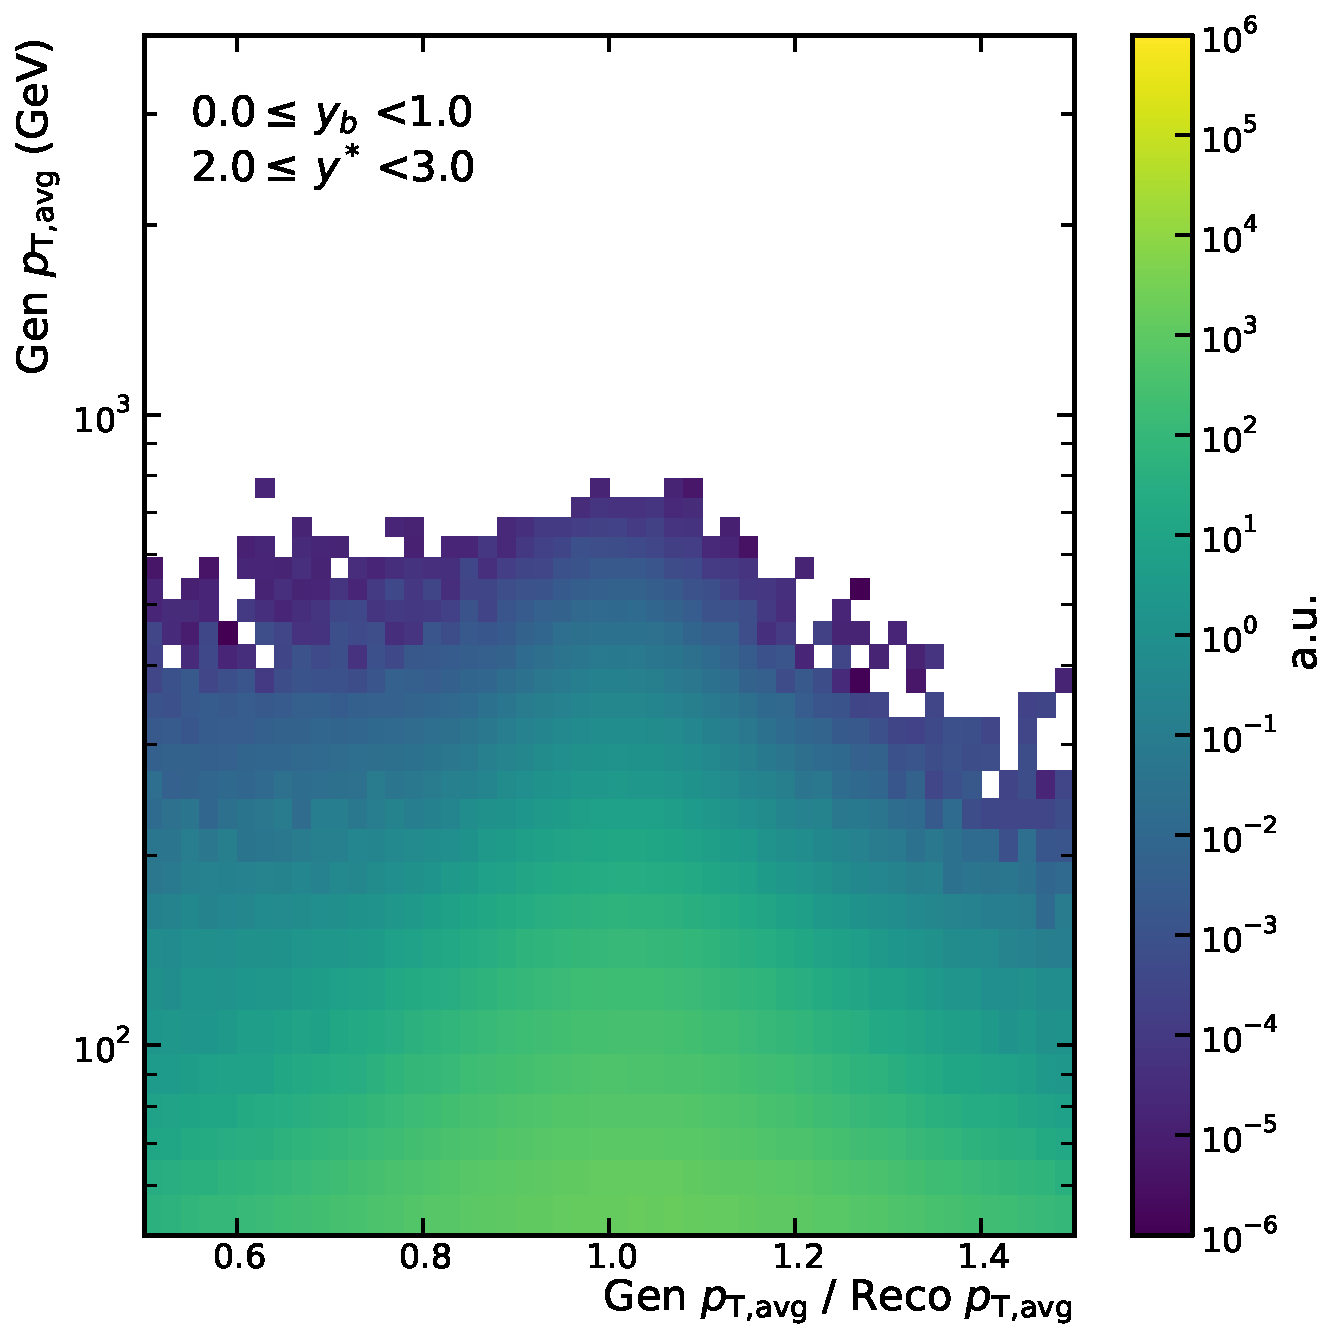
\includegraphics[width=0.45\textwidth]{figures/measurement/gen_vs_reco_vs_gen_ptavg_yb0ys2.pdf}\hfill
    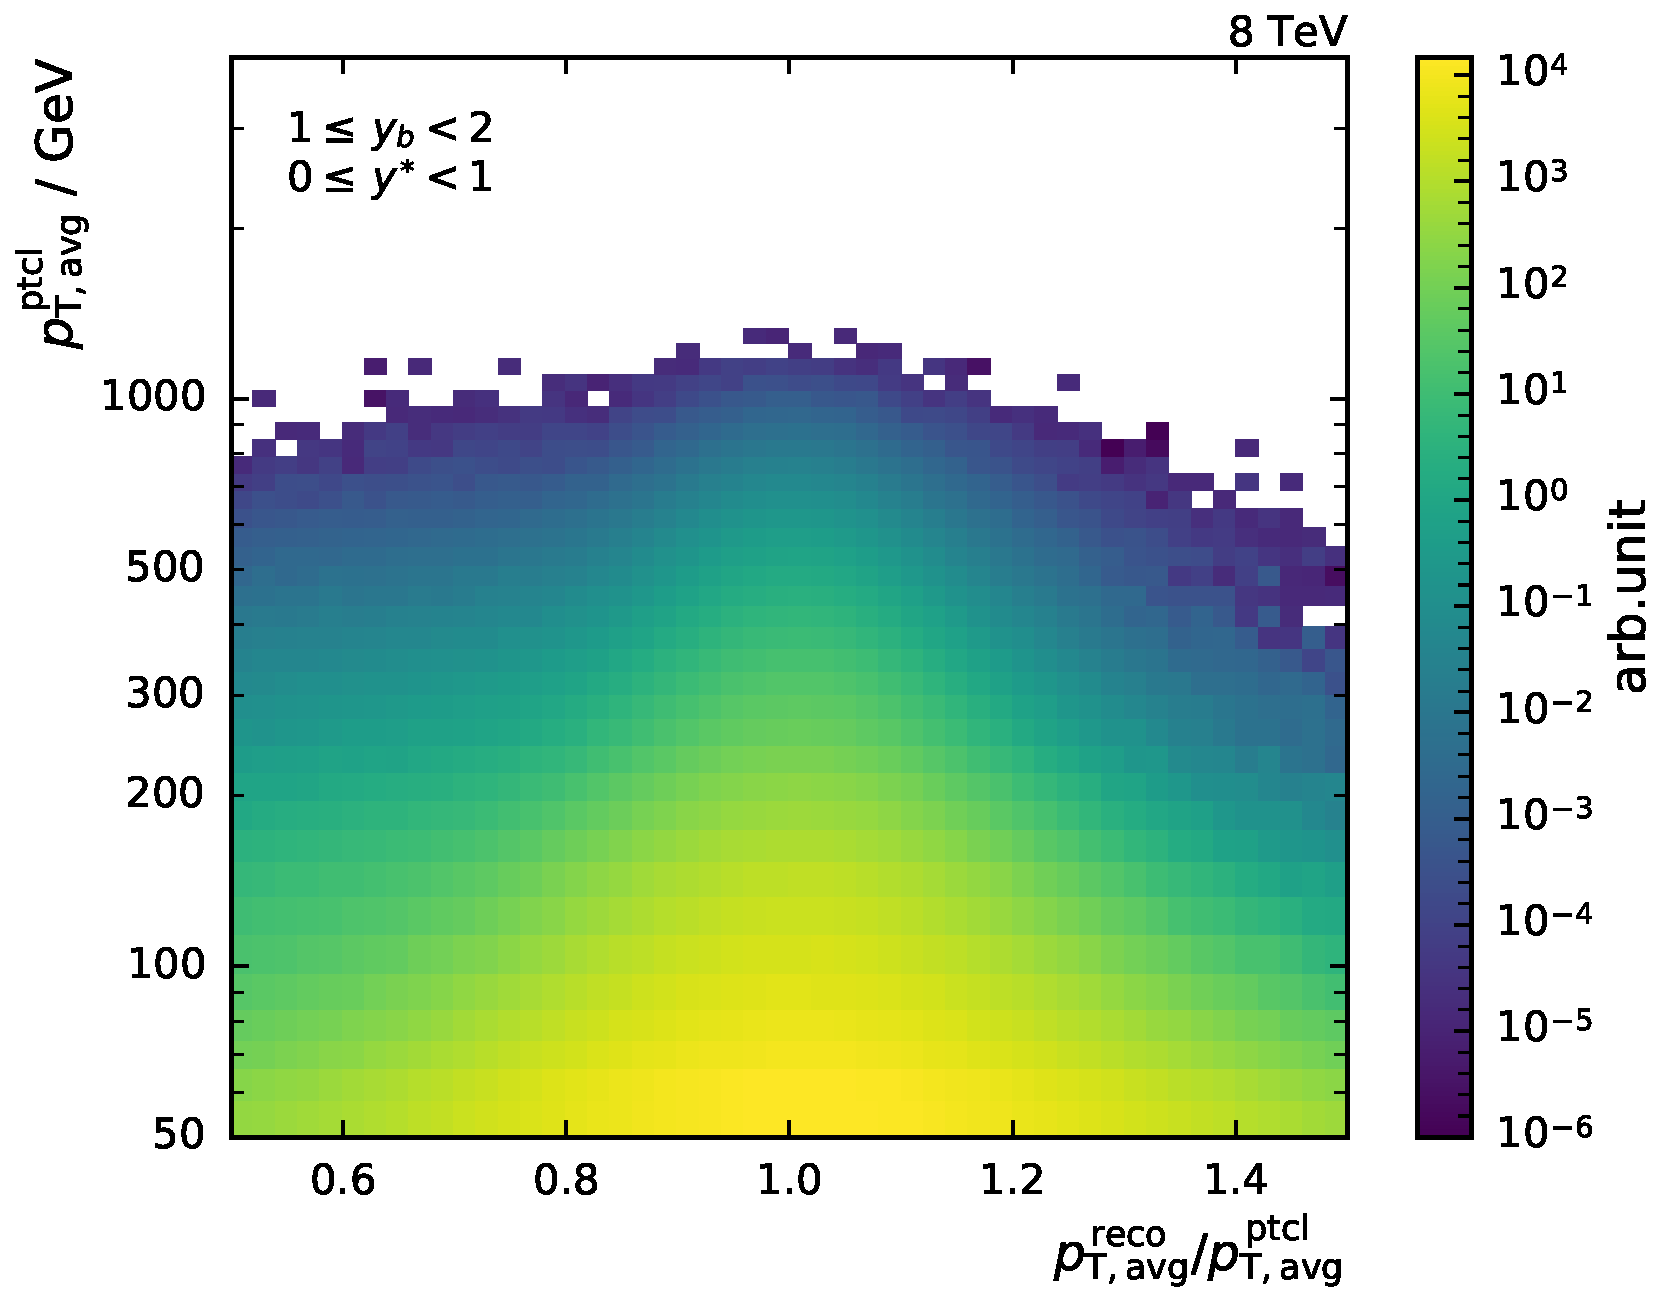
\includegraphics[width=0.45\textwidth]{figures/measurement/gen_vs_reco_vs_gen_ptavg_yb1ys0.pdf}
    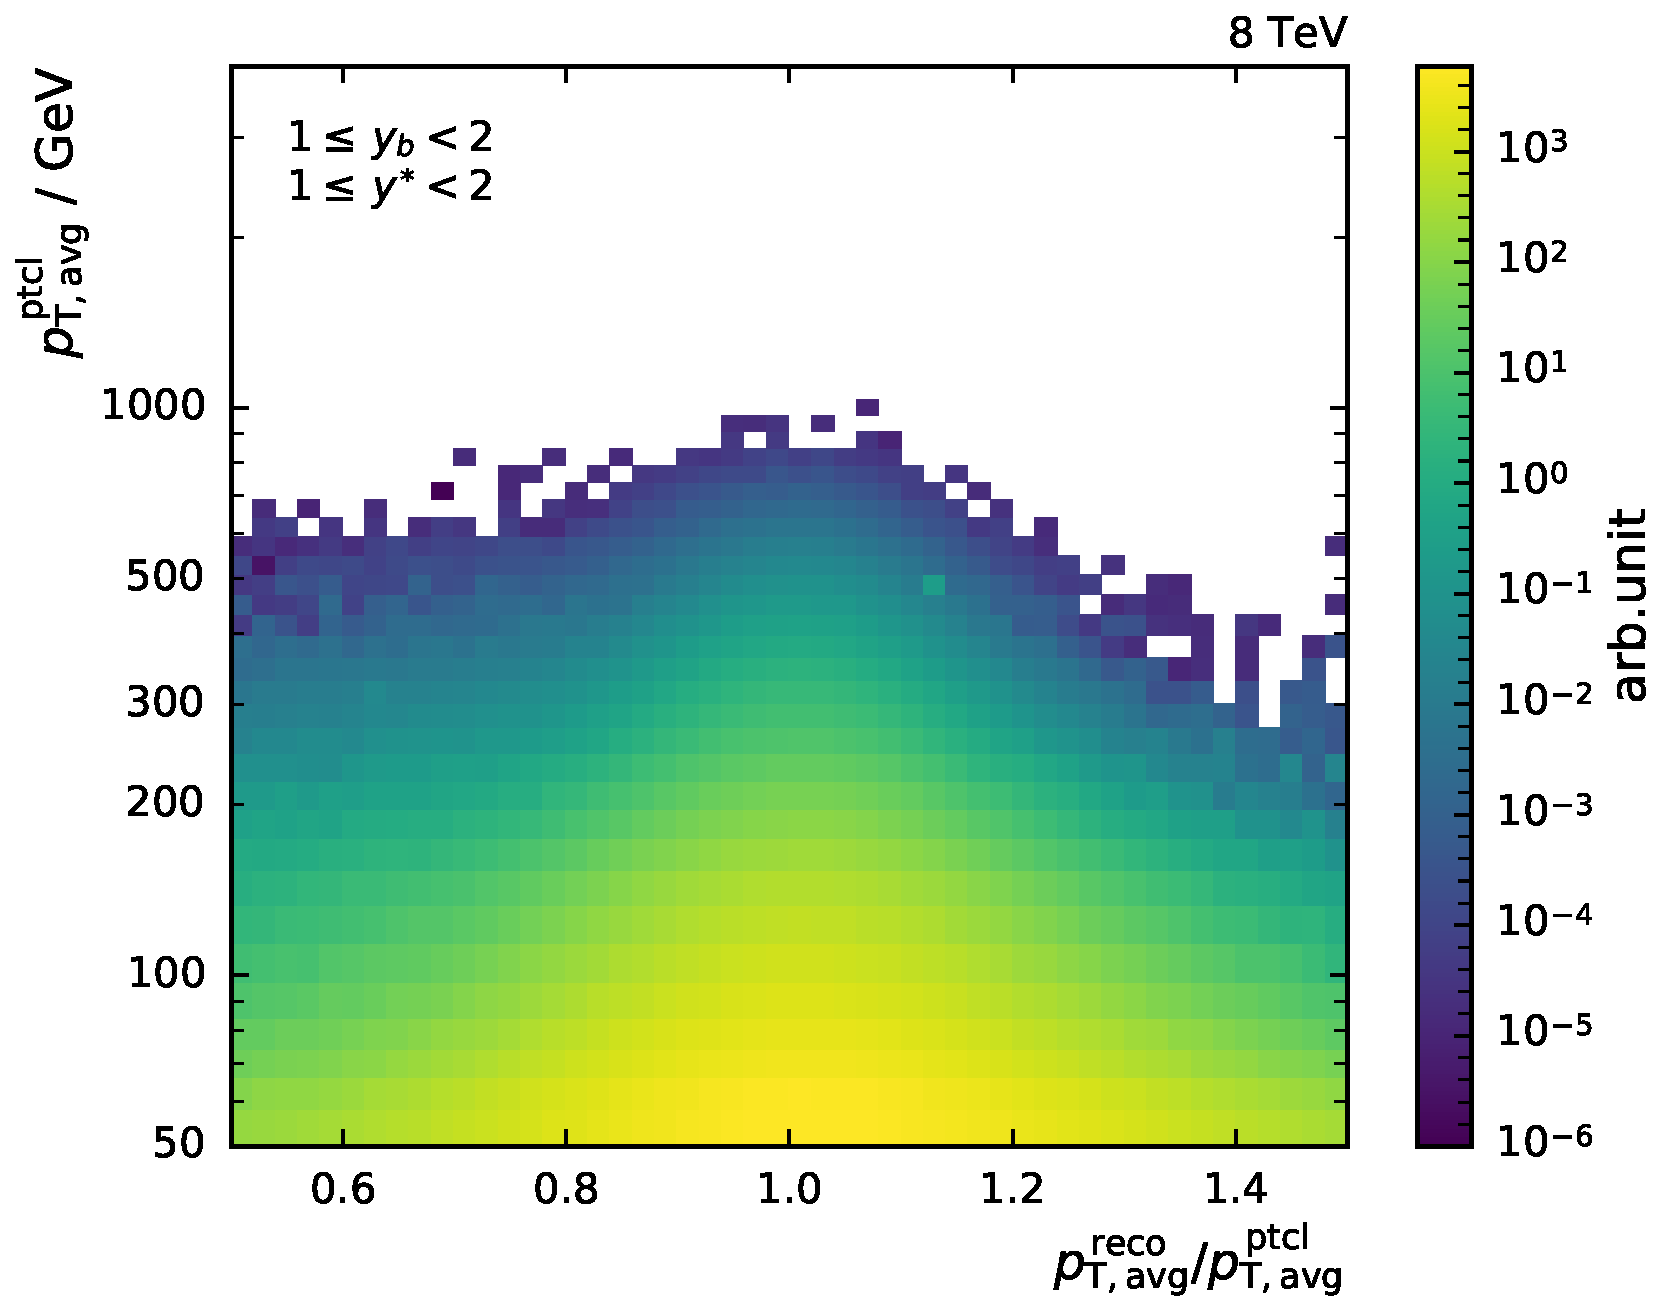
\includegraphics[width=0.45\textwidth]{figures/measurement/gen_vs_reco_vs_gen_ptavg_yb1ys1.pdf}\hfill
    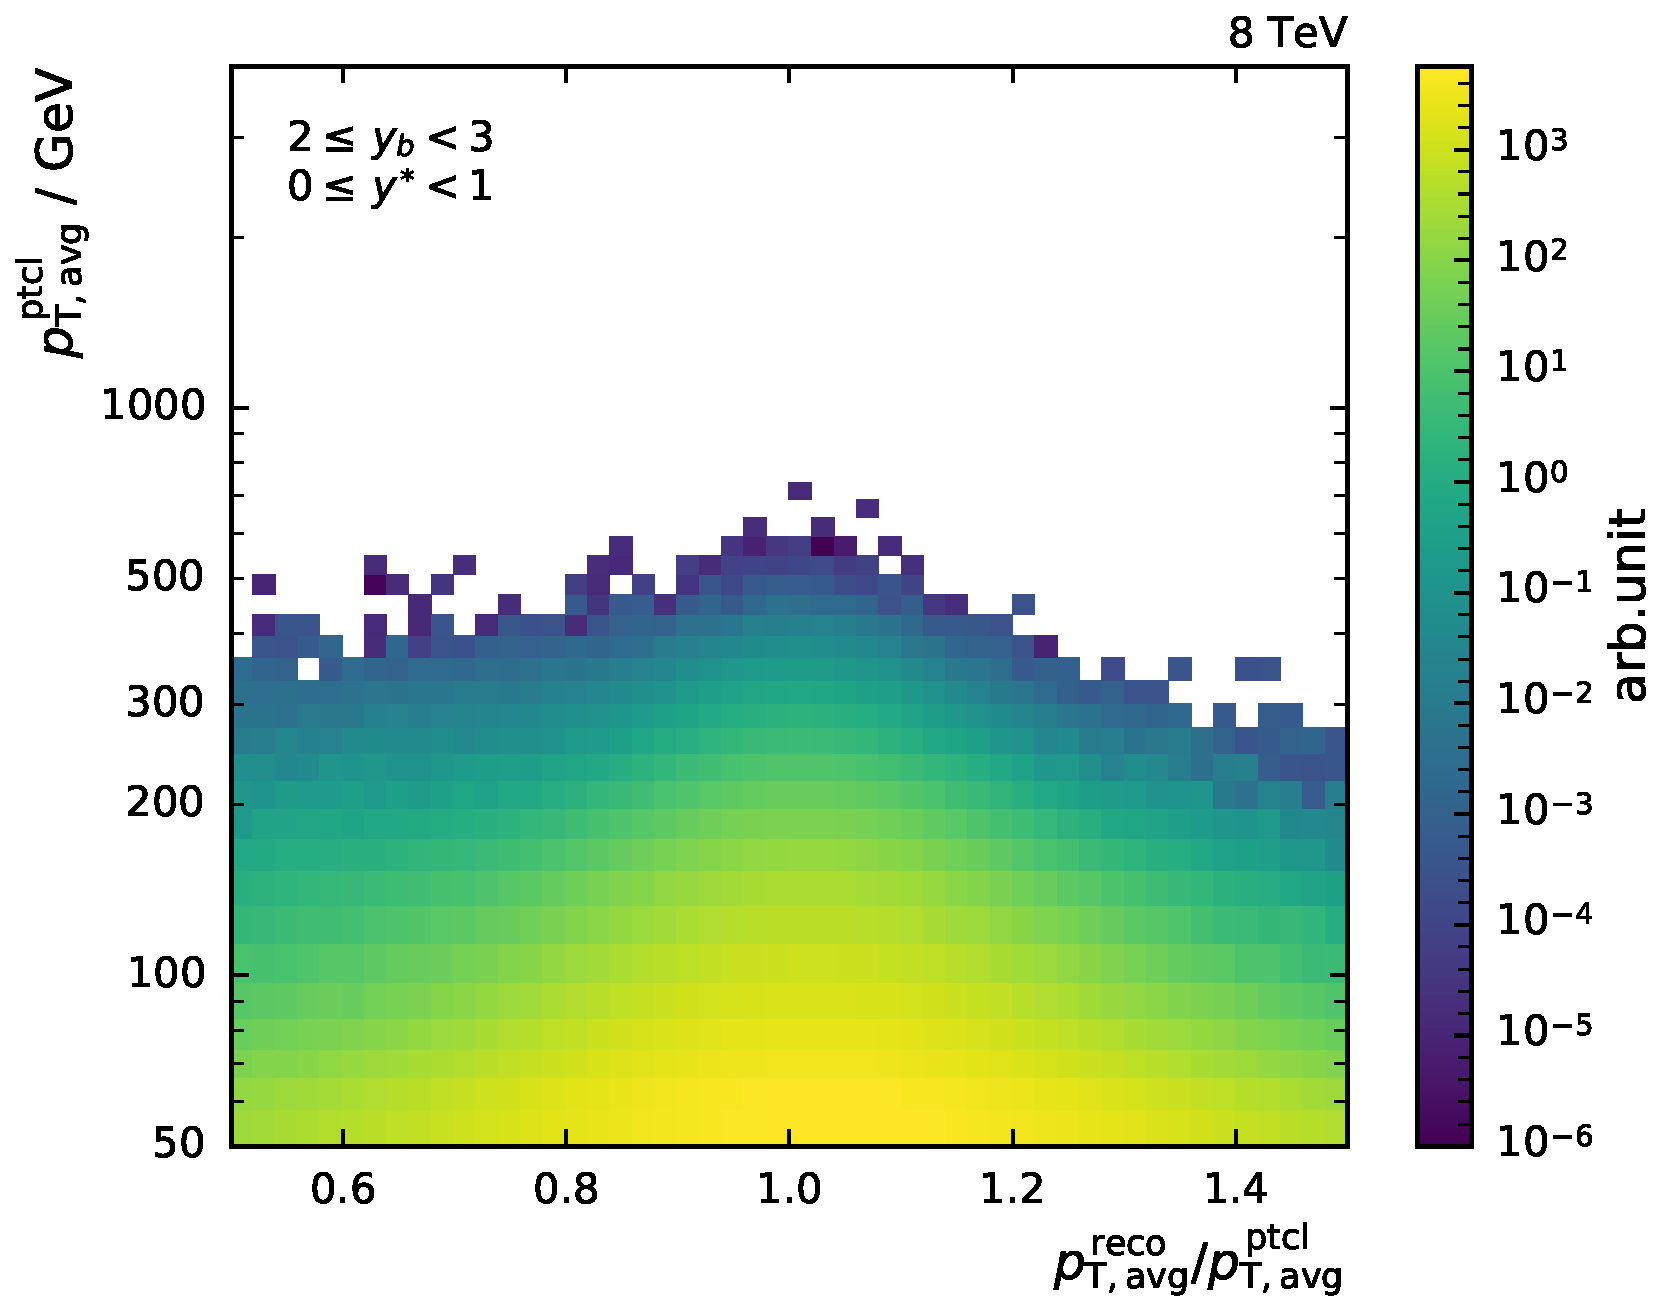
\includegraphics[width=0.45\textwidth]{figures/measurement/gen_vs_reco_vs_gen_ptavg_yb2ys0.pdf}
    \caption[Comparison generated vs. reconstructed transverse energy]{The
    average transverse momentum generated as a function of the ratio of
generated and reconstructed \ptavg. The width of the distribution indicating the
jet energy resolution improves for higher values of \ptavg as expected. The
resolution is extracted for each bin separately.}
    \label{fig:gen_vs_reco_over_gen}
\end{figure}

Figure~\ref{fig:resolution_bin} shows the distribution for one \ptavg bin. The
width is fitted using a gaussian function. The non-gaussian tails, visible in
the logarithmic representation, were found to not influence the resulting
resultion. The width of the distributions in each /ptavg is then shown as a
function of \ptavg. Figure~\ref{fig:resolution_ptavg} shows the final relative
resolution for each \ystar and \yboost bin. The relative resolution is described
by a modified version of the NSC formula.

\begin{equation}
    \frac{\sigma_{\text{ptavg}}}{\ptavg} (\ptavg) = \sqrt{\sgn{N} \left(\frac{N}{\ptavg}\right)^2 + \left(\frac{\ptavg}{\text{GeV}}\right)^s \frac{S^2}{\ptavg} + C^2 }
    \label{eq:resolution}
\end{equation}

\begin{figure}[htbp]
    \centering
    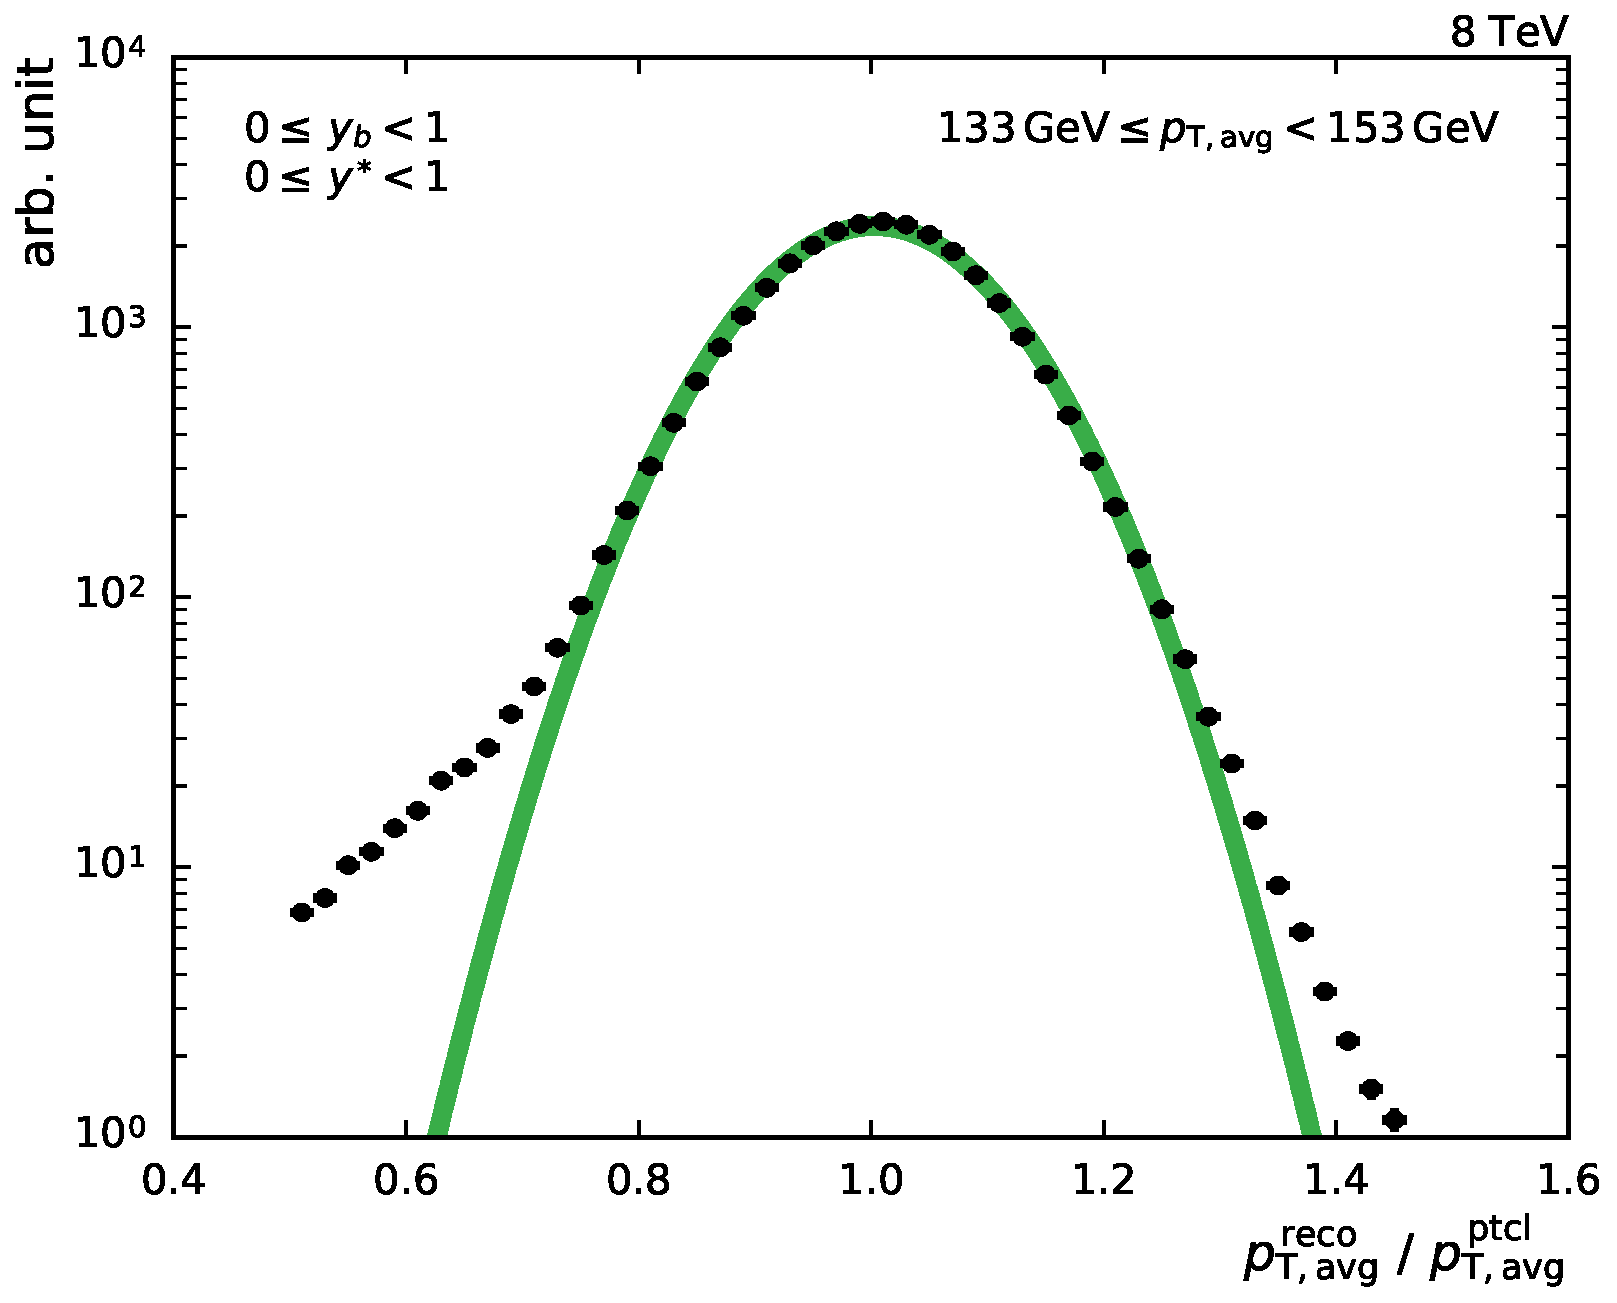
\includegraphics[width=0.5\textwidth]{figures/measurement/resolution_yb0ys0_bin10.pdf}
    \caption{Dijet \ptavg resolution}
    \label{fig:resolution_bin}
\end{figure}


\begin{figure}[htbp]
    \centering
    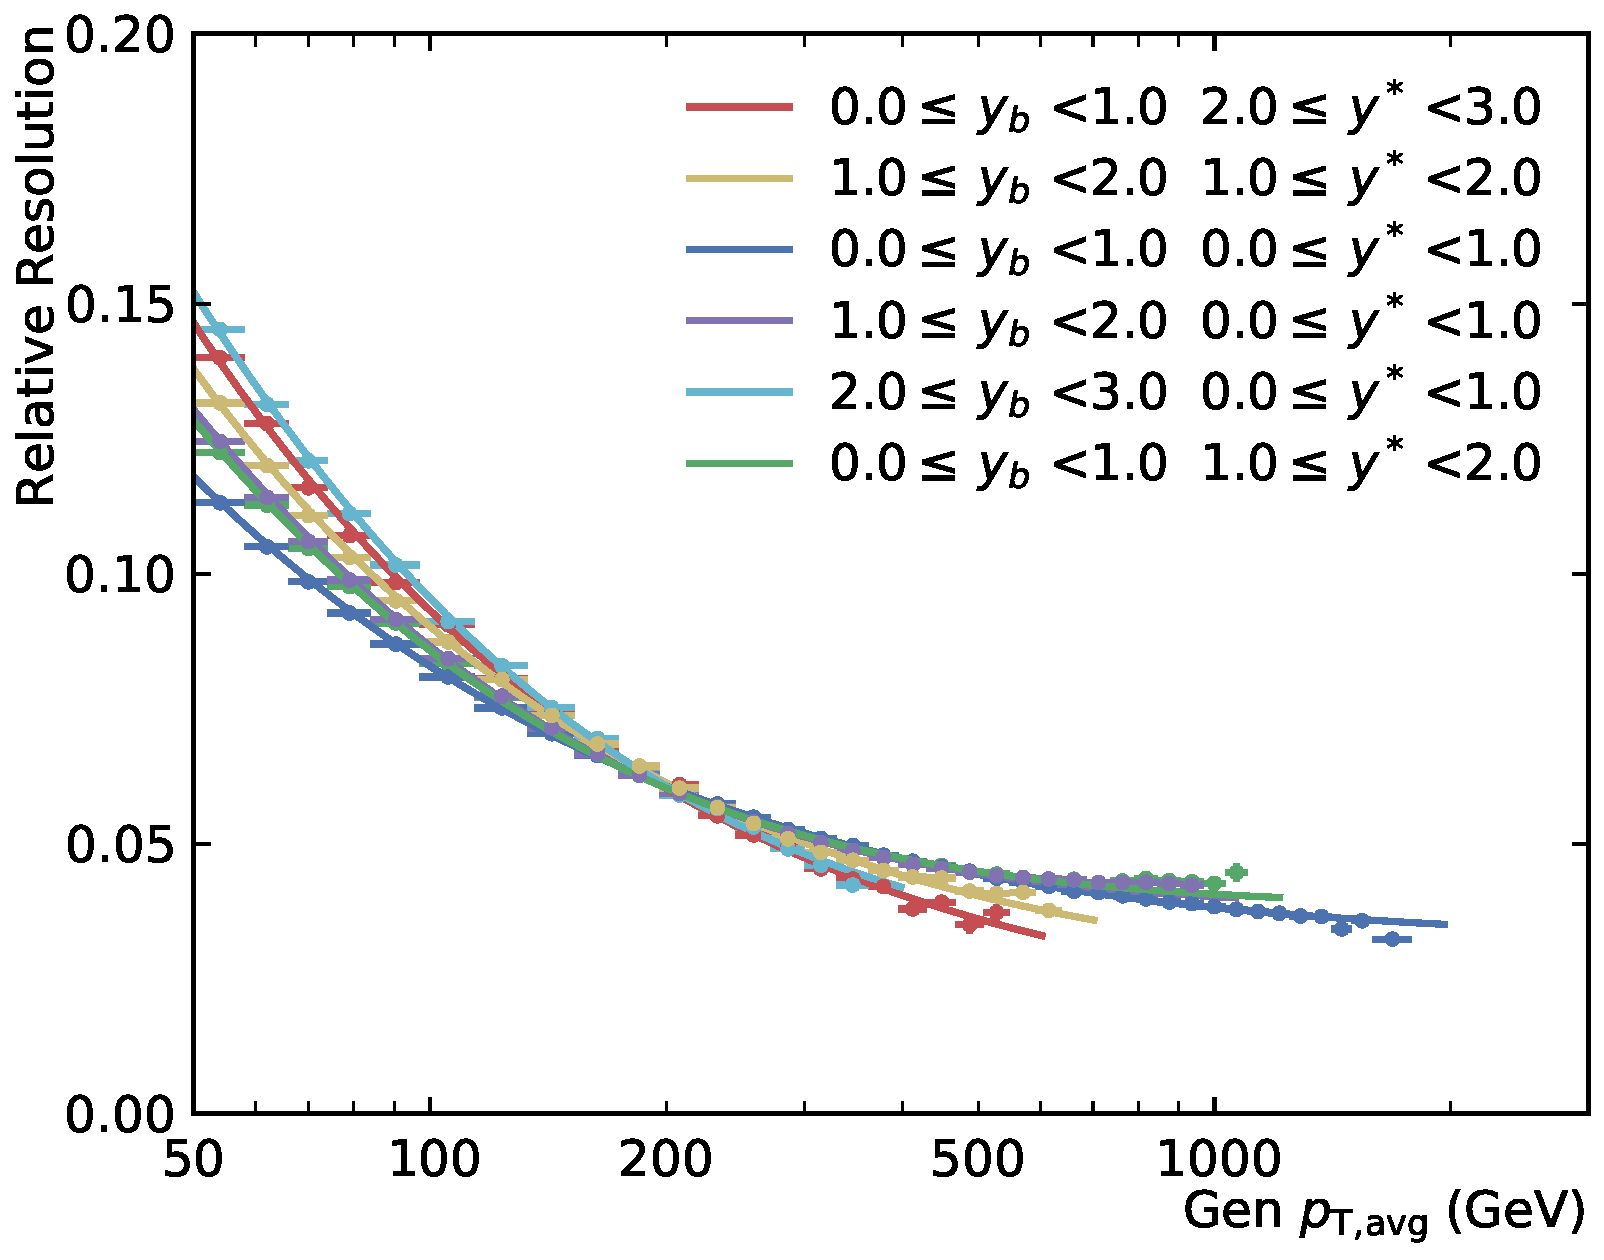
\includegraphics[width=0.5\textwidth]{figures/measurement/resolution_ptavg.pdf}
    \caption{Dijet \ptavg resolution}
    \label{fig:resolution_ptavg}
\end{figure}

The formula is based on the usual NSC formula which describes the resolution in
terms of noise $N$, a stochastic component $S$ and a constant term $C$.
Especially in the low-\pt region in which the tracking has a non-negligible
influence on the resolution due to the particle flow algorithm, a slightly
better fit is obtained by using the modified resolution
formula~\ref{eq:resolution}. Table~\ref{tab:resolution_parameters} gives the
parameters of the fit in each bin of the measurement.

\begin{table}[htbp]
    \centering
    \caption[Relative dijet transverse momentum resolution parameters]{The parameters of the resolution fit are shown for each bin in \ystar and \yboost.}
    \label{tab:resolution_parameters}
    \begin{tabular}{cccccr}
        \toprule
         \yboost & \ystar & N      & S     & C      & s\\\midrule
         0 -- 1  & 0 -- 1 & -6.26  & 3.62  & 0.05   & -0.43\\
         0 -- 1  & 1 -- 2 & -25.96 & 23.05 & 0.05   & -0.91\\
         0 -- 1  & 2 -- 3 & -6.56  & 4.02  & -0.017 & -0.43\\
         1 -- 2  & 0 -- 1 & -28.33 & 25.51 & 0.05   & -0.92\\
         1 -- 2  & 1 -- 2 & -5.79  & 3.13  & 0.03   & -0.35\\
         2 -- 3  & 0 -- 1 & -7.12  & 3.967 & 0.00   & -0.41\\\hline
            \bottomrule
    \end{tabular}
\end{table}

\section{Unfolding of the Measurement}
\label{sec:unfolding}

The final goal is the comparison of the triple-differential dijet cross section
with higher-order QCD calculations. Due to the finite detector acceptance and resolution
the measured spectrum is smeared causing differences between the true dijet \ptavg distribution
and the measured distribution. To accomplish that goal, the measurement has
to be unfolded to yield the result at particle level. Thus all future Monte-Carlo event
generators can be easily compared with this measurement without needing to apply
the detector simulation.

In this analysis, the iterative d'Agostini algorithm~\cite{DAgostini:1994zf} which is
implemented in the RooUnfold~\cite{Adye:2011gm} package is used. The unfolding
process is regularized by the number of interation steps in this algorithm. A
higher number of iterations yields a better reduced \chisq but also increases
the uncertainty and introduces larger bin-by-bin fluctuations and correlations.
The regularization was optimized using a Monte-Carlo data sample and best
results with low bin-by-bin correlations and a low \chisq were achieved using
four iterations in the unfolding algorithm.

In principal, the response matrix for the unfolding algorithm can be directly
filled using the Monte-Carlo generated events containing the thue and measured
information. However this method has several drawbacks. The LO prediction not
neccesarily describes the shape of the distribution in all cases. Additionally
the limited number of events in the Monte-Carlo sample, especially at high
rapidities and high transverse momentum, introduces large statistical
fluctuations in the response matrix. Because of these undesired effects a
different stategy is employed to populate the response matrix.

Based on the good description of the data spectrum by NLO predictions, a forward
smearing is applied. At first, the NLO prediction obtained with the CT14-NLO PDF
set and corrected for non-perturbative effects, is fitted using the function

\begin{equation}
    f(\ptavg) = A_0 \left(
    \frac{\ptavg}{A_3}\right)^{-A_1}\left(1-\frac{\ptavg}{A_3}\right)^{A_2}
\end{equation}

Using a Toy MC method a flat \ptavg spectrum is generated, which is weighted
according to the NLO distribution. The distribution of this generated sample
resembles the fastNLO cross section prediction and is used as the true \ptavg
spectrum. The generated events are smeared using the resolution function
measured in Section~\ref{sec:resolution}. The generation of these Monte-Carlo
toy events is very fast, and the response matrices are filled with around 100
million events each resulting in negligible statistical fluctuations.
Figure~\ref{fig:res_matrix} shows the response matrices used in the unfolding
process. The matrices in the figure are normalized to number of gen events in
each row to improve the readibility. The response matrices are diagonal with
small off-diagonal migrations between close-by \ptavg bins.

\begin{figure}[htp]
    \centering
    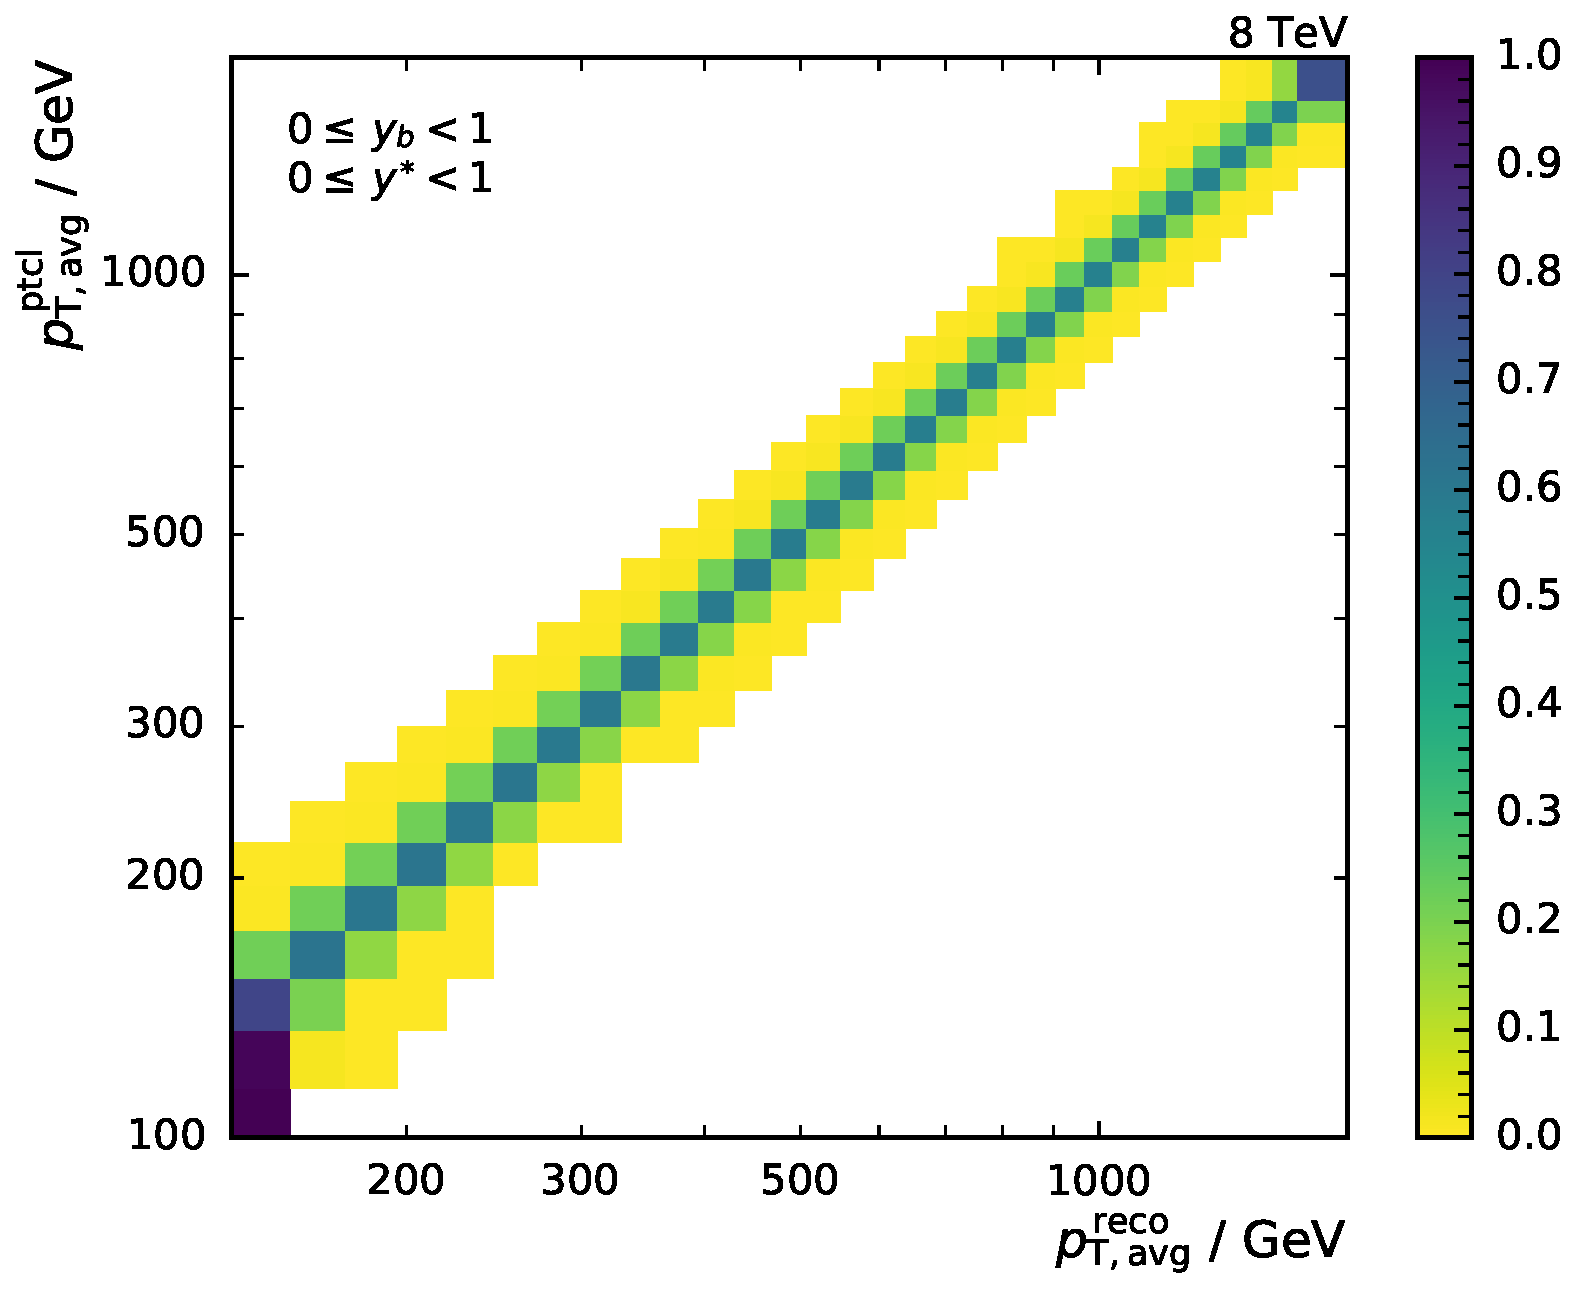
\includegraphics[width=0.45\textwidth]{figures/measurement/res_matrix_ptavg_normalized_yb0ys0.pdf}\hfill
    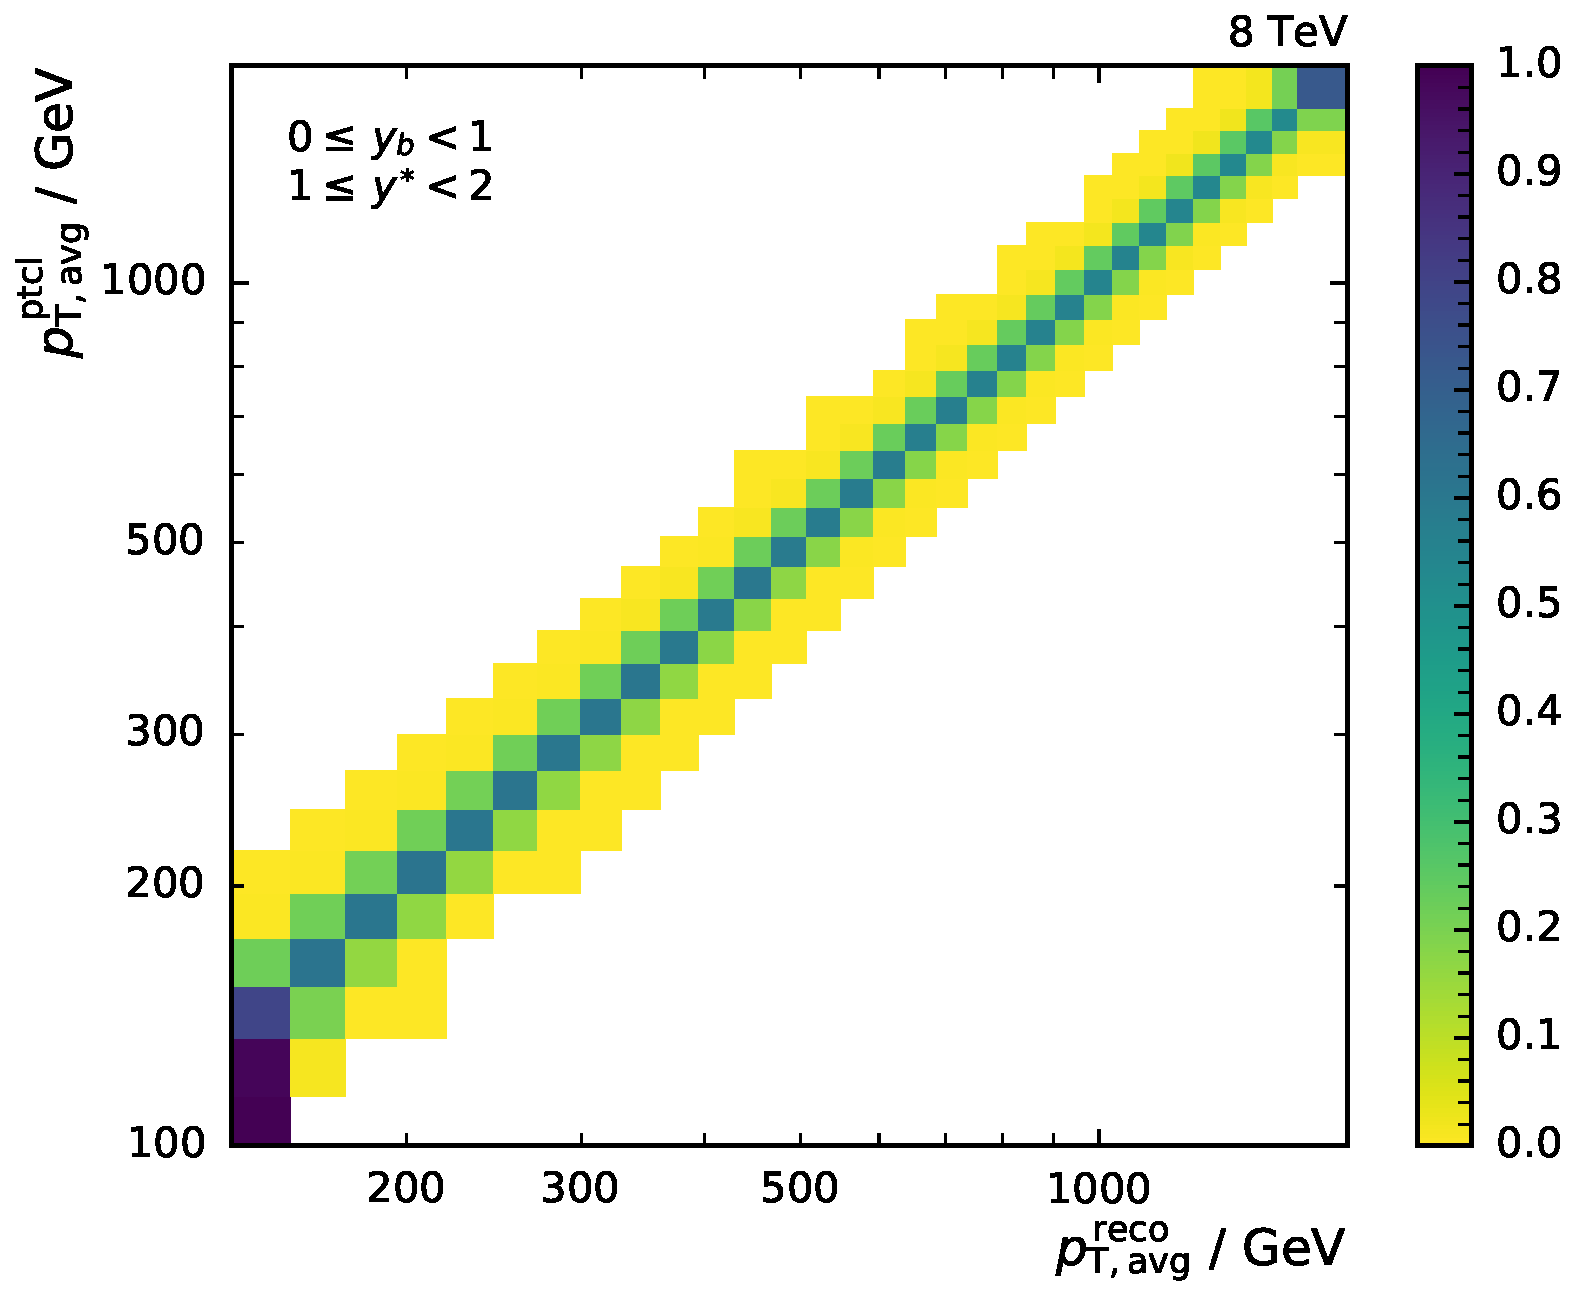
\includegraphics[width=0.45\textwidth]{figures/measurement/res_matrix_ptavg_normalized_yb0ys1.pdf}
    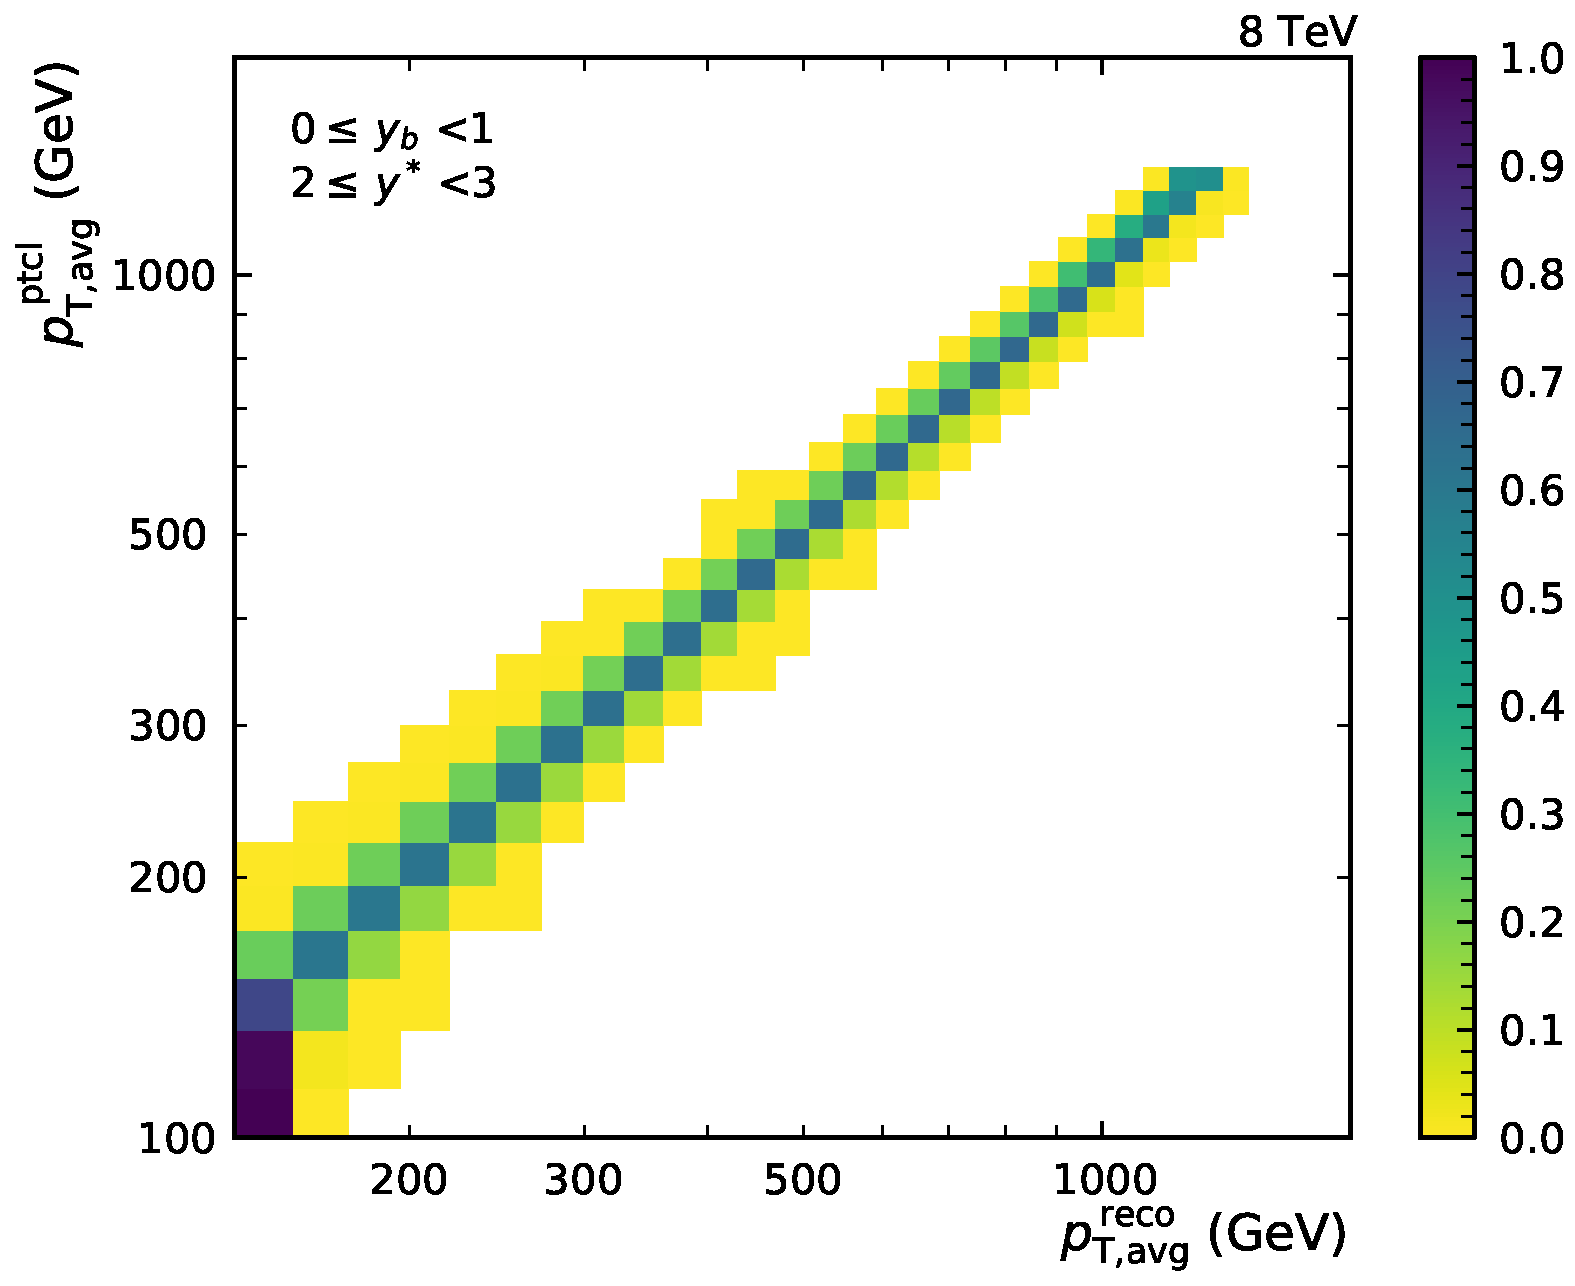
\includegraphics[width=0.45\textwidth]{figures/measurement/res_matrix_ptavg_normalized_yb0ys2.pdf}\hfill
    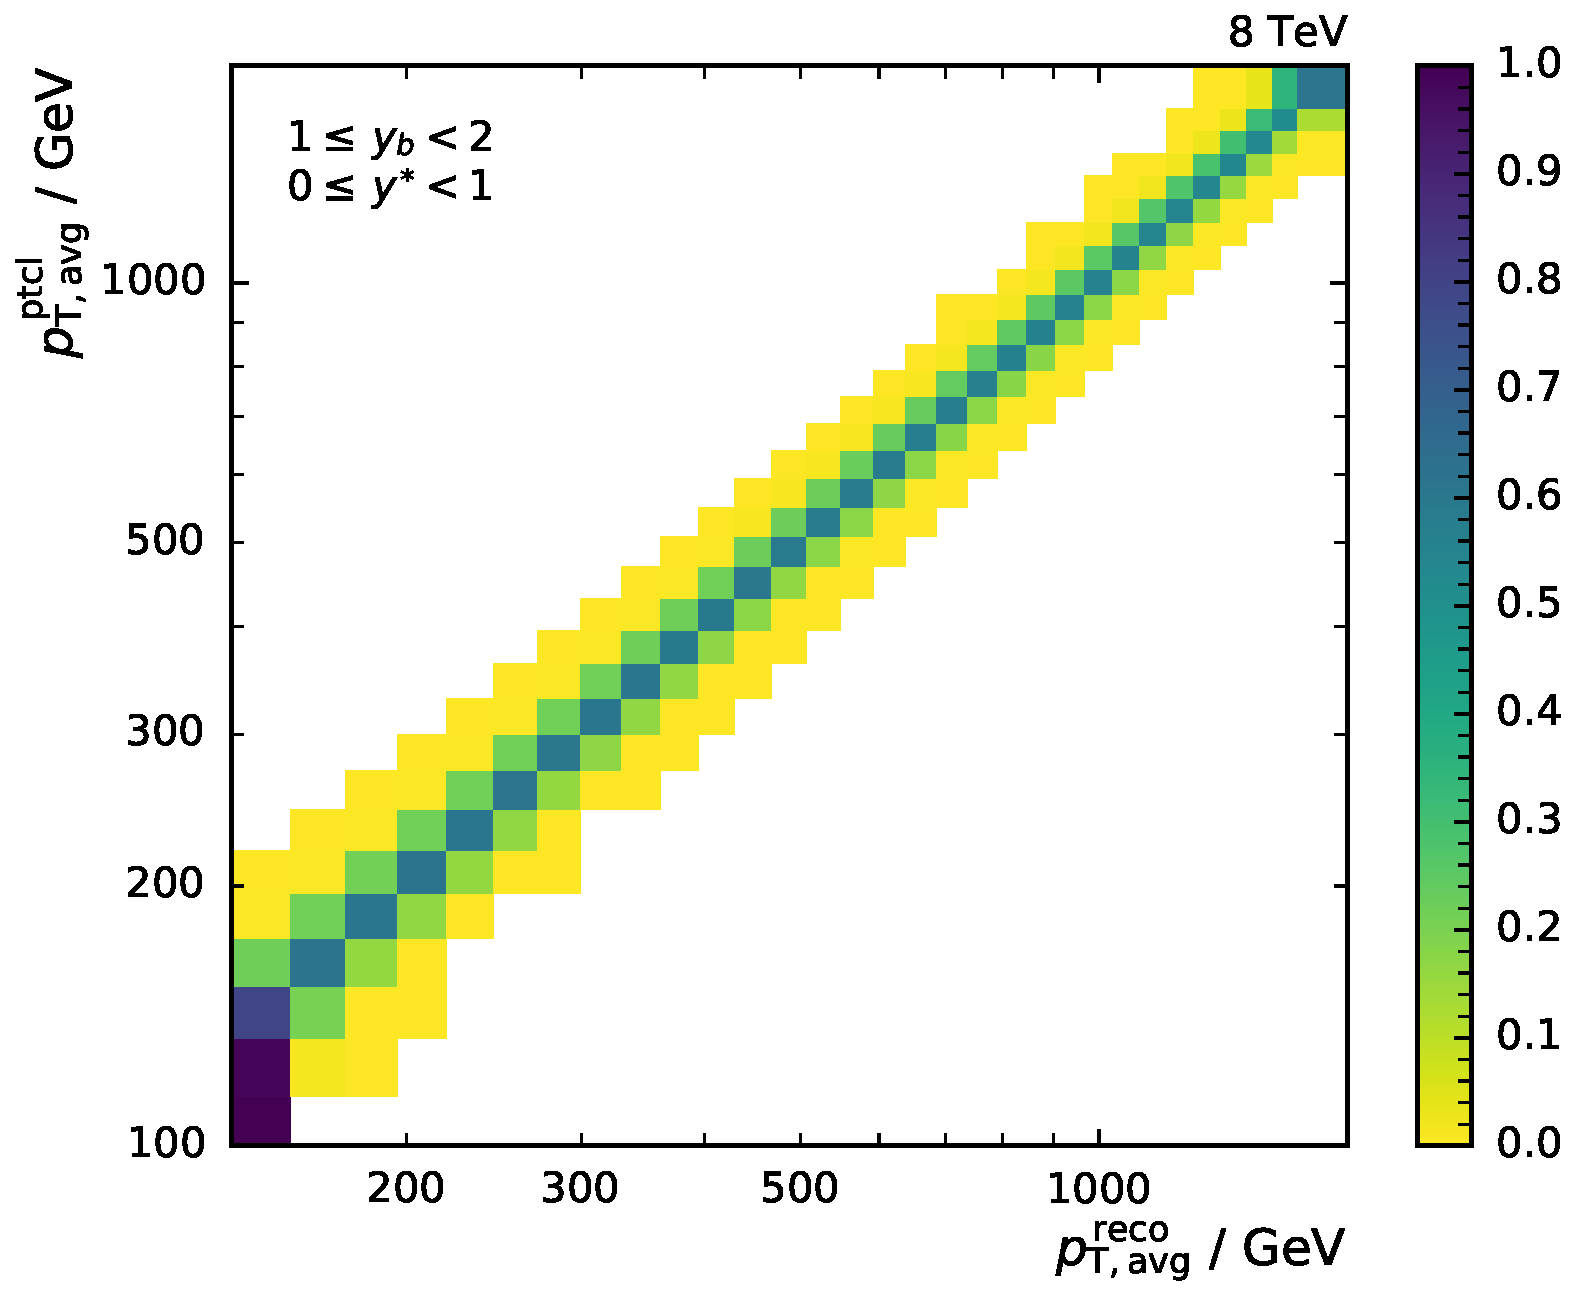
\includegraphics[width=0.45\textwidth]{figures/measurement/res_matrix_ptavg_normalized_yb1ys0.pdf}
    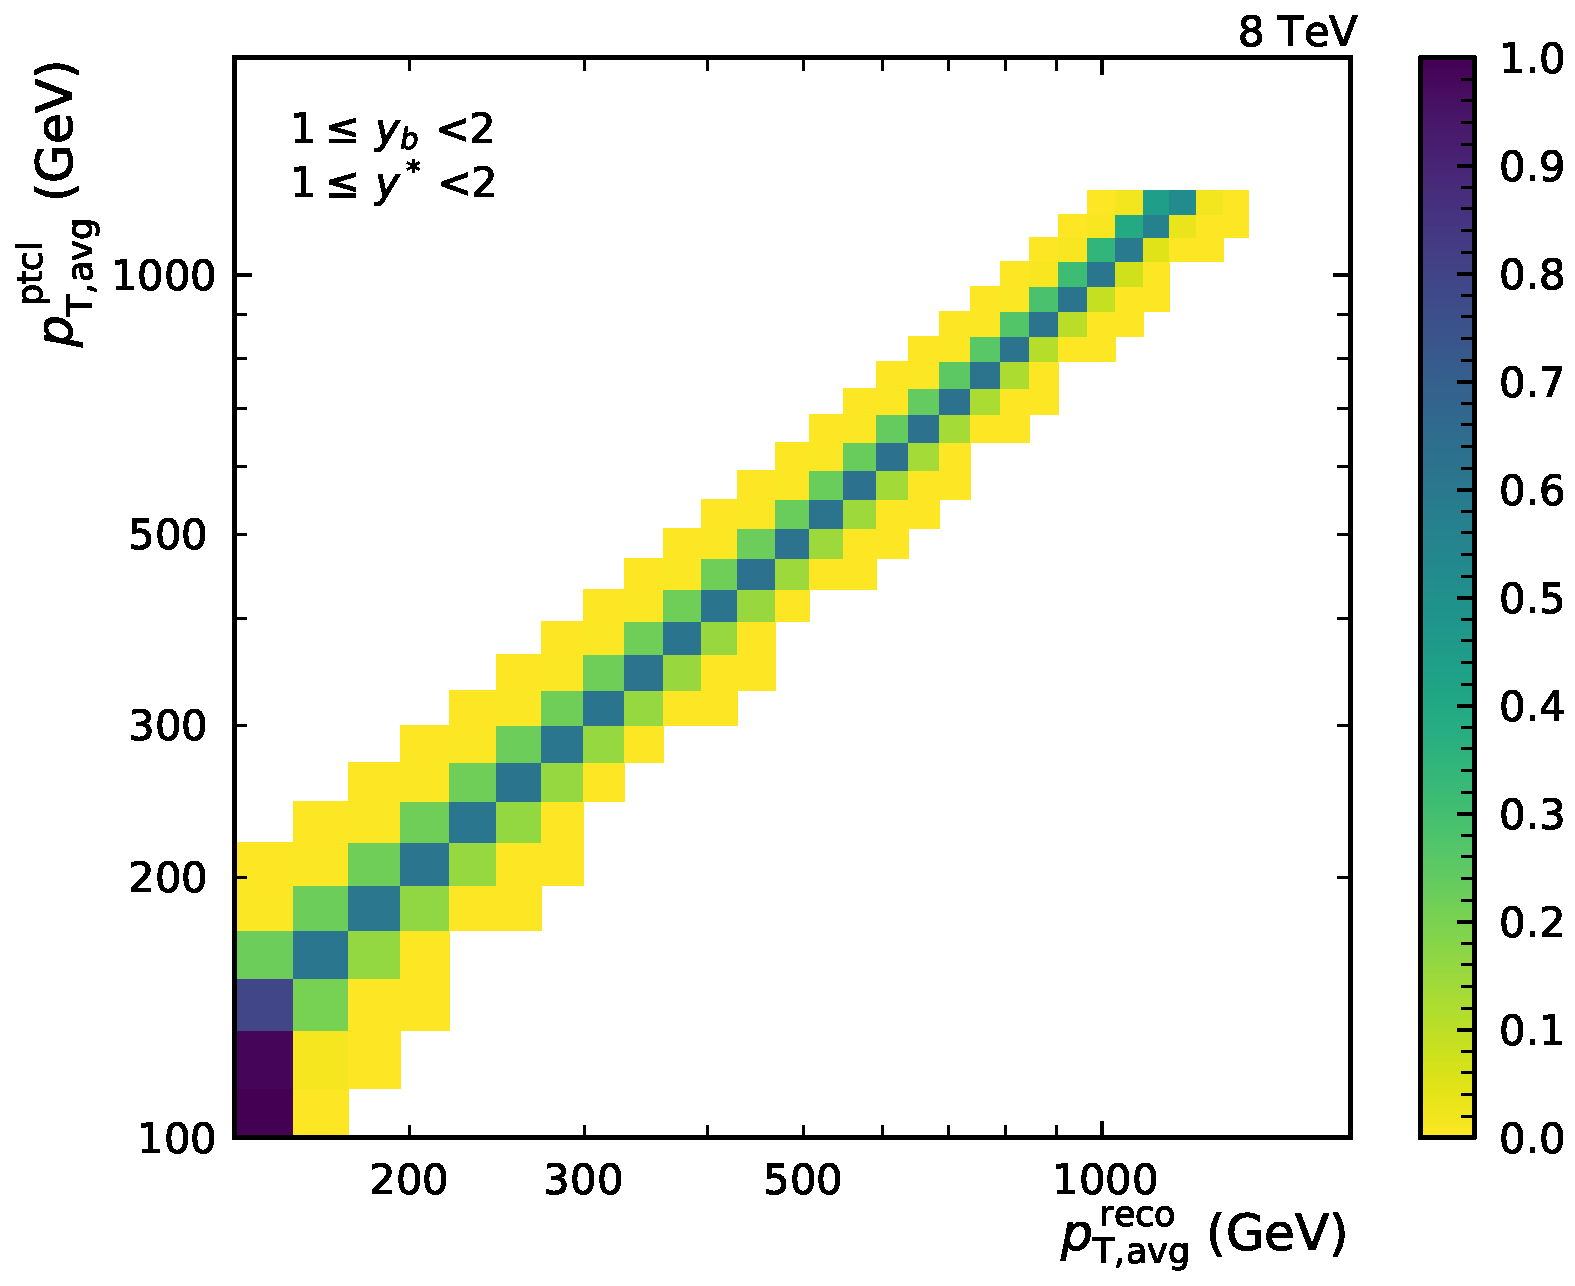
\includegraphics[width=0.45\textwidth]{figures/measurement/res_matrix_ptavg_normalized_yb1ys1.pdf}\hfill
    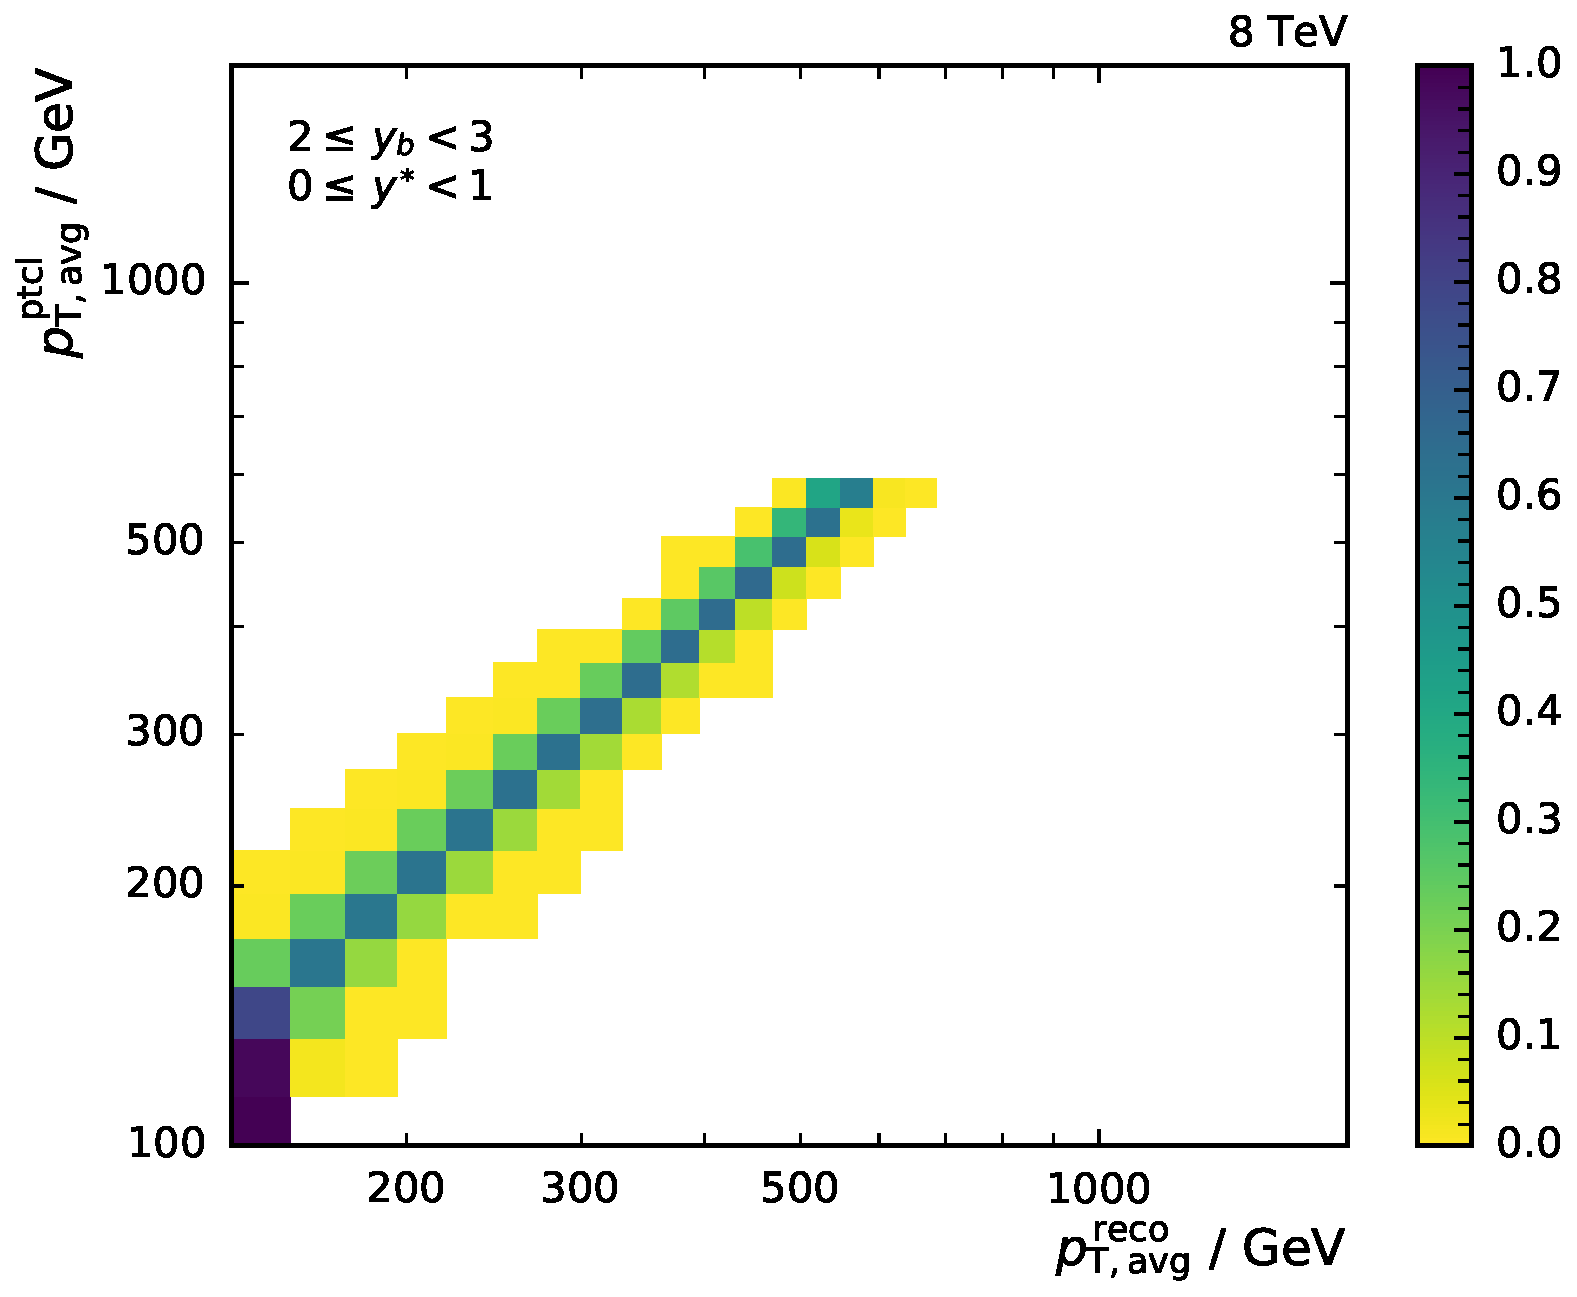
\includegraphics[width=0.45\textwidth]{figures/measurement/res_matrix_ptavg_normalized_yb2ys0.pdf}
    \caption[Response matrix used for the unfolding procedure]{Response matrix used for the unfolding procedure. The response matrices are obtained
            using the smearing method and are normalized to the number of gen events in each row to improve
            the readibility.}
    \label{fig:res_matrix}
\end{figure}

A closure test was performed by applying the unfolding using response matrices
filled directly from the Monte-Carlo samples and from the generated and smeared
toy events. It was found that the results agree in both cases within statistical
uncertainties.

Additionally it was studied that the bin-by-bin migration between phase space
bins in \ystar and \yboost are small and the effects neglibible. Thereby it is
justified to perform the unfolding in each \ystar and \yboost bin separately and
to not perform a three-dimensional unfolding which is much more cumbersome.

The statistical uncertainties of the data distributions are propagated through
the unfolding procedure using toy experiments. The procedure as well as the
results are discussed in detail in Sec.~\ref{sec:stat_unf_uncert}.


\section{Experimental Uncertainties}
\label{experimental_uncertainties}

This section presents the derivation of all experimental sources of uncertainty
which affect the cross section measurement. The comprehensive uncertainty
studies involve the statistical uncertaint which was propagated through the
unfolding, the luminosity uncertainty arising from the imperfection of the CMS
luminosity, the jet energy correction uncertainty due to the calibration of the
jet energy energy and the uncertainty of the jet energy resolution measurement.
Furthermore an uncorrelated residual uncertainty of 1\%, which comprises the
trigger efficiency uncertainty, the jet id efficiency and further residual
effects, is considered.

Fig.~\ref{fig:exp_unc_overview} shows all sources of experimental uncertainty as
well as the total uncertainty, obtained by adding in quadrature the individual
sources. The total uncertainty is 8\% in the measurement bins involving jets at
central rapidity and increases up to 20\% in bins involving jets in the less
well understood forward region.

\todo{table exp uncertainties}

\subsection {Uncertainty on Luminosity Measurement}

As discussed in Sec.~\ref{sec:lumi_measurement}, the luminosity is measured from
the number of clusters in the silicon pixel detector. The integrated luminosity
for the selected data in the 2012 LHC run is determined to be \SI{19.71}{\per
\femto \barn}. 

The uncertainty on the luminosity measurement for the 2012 LHC run is estimated
to be 2.5\% (syst.) and 0.5\% (stat.)~\cite{CMS-PAS-LUM-13-001}. The luminosity
uncertainty afffects the normalization of any absolute cross section measurement
and is therefore taken into account.

\subsection{Unfolding and Statistical Uncertainty}
\label{sec:stat_unf_uncert}

The statistical uncertainties of the data distributions are are propagated
through the unfolding using a toy MC procedure in which the measured histogram
is smeared according to its statistical uncertainty and the unfolding procedure
is performed multiple times for each of these smeared spectra. A million
generated toy spectra are used to propagate the statistical uncertainty.
Figure~\ref{fig:statunc_relative} shows the relative statistical uncertainty before and
after the unfolding procedure. The uncertainty slightly increases during the unfolding
process as it is expected.

\begin{figure}[htbp]
    \centering
    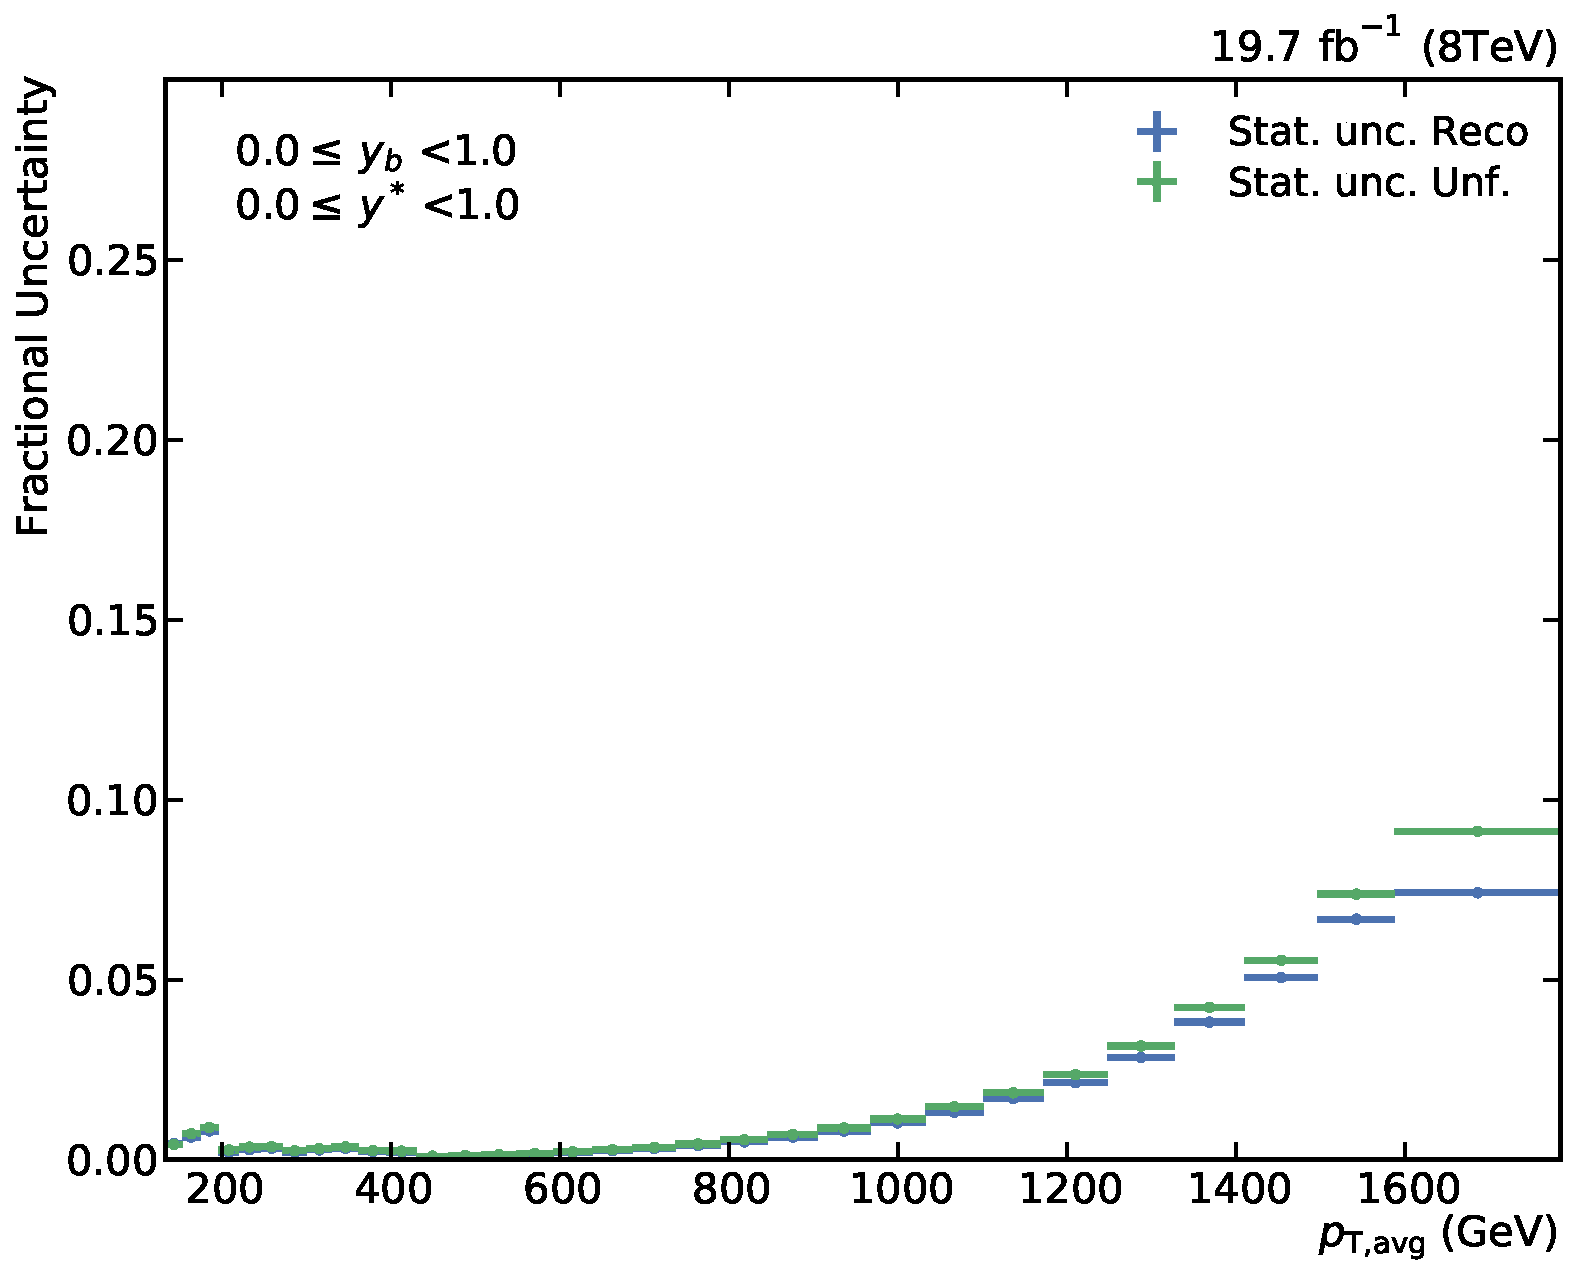
\includegraphics[width=0.45\textwidth]{figures/measurement/statunc_fractional_yb0ys0.pdf}\hfill
    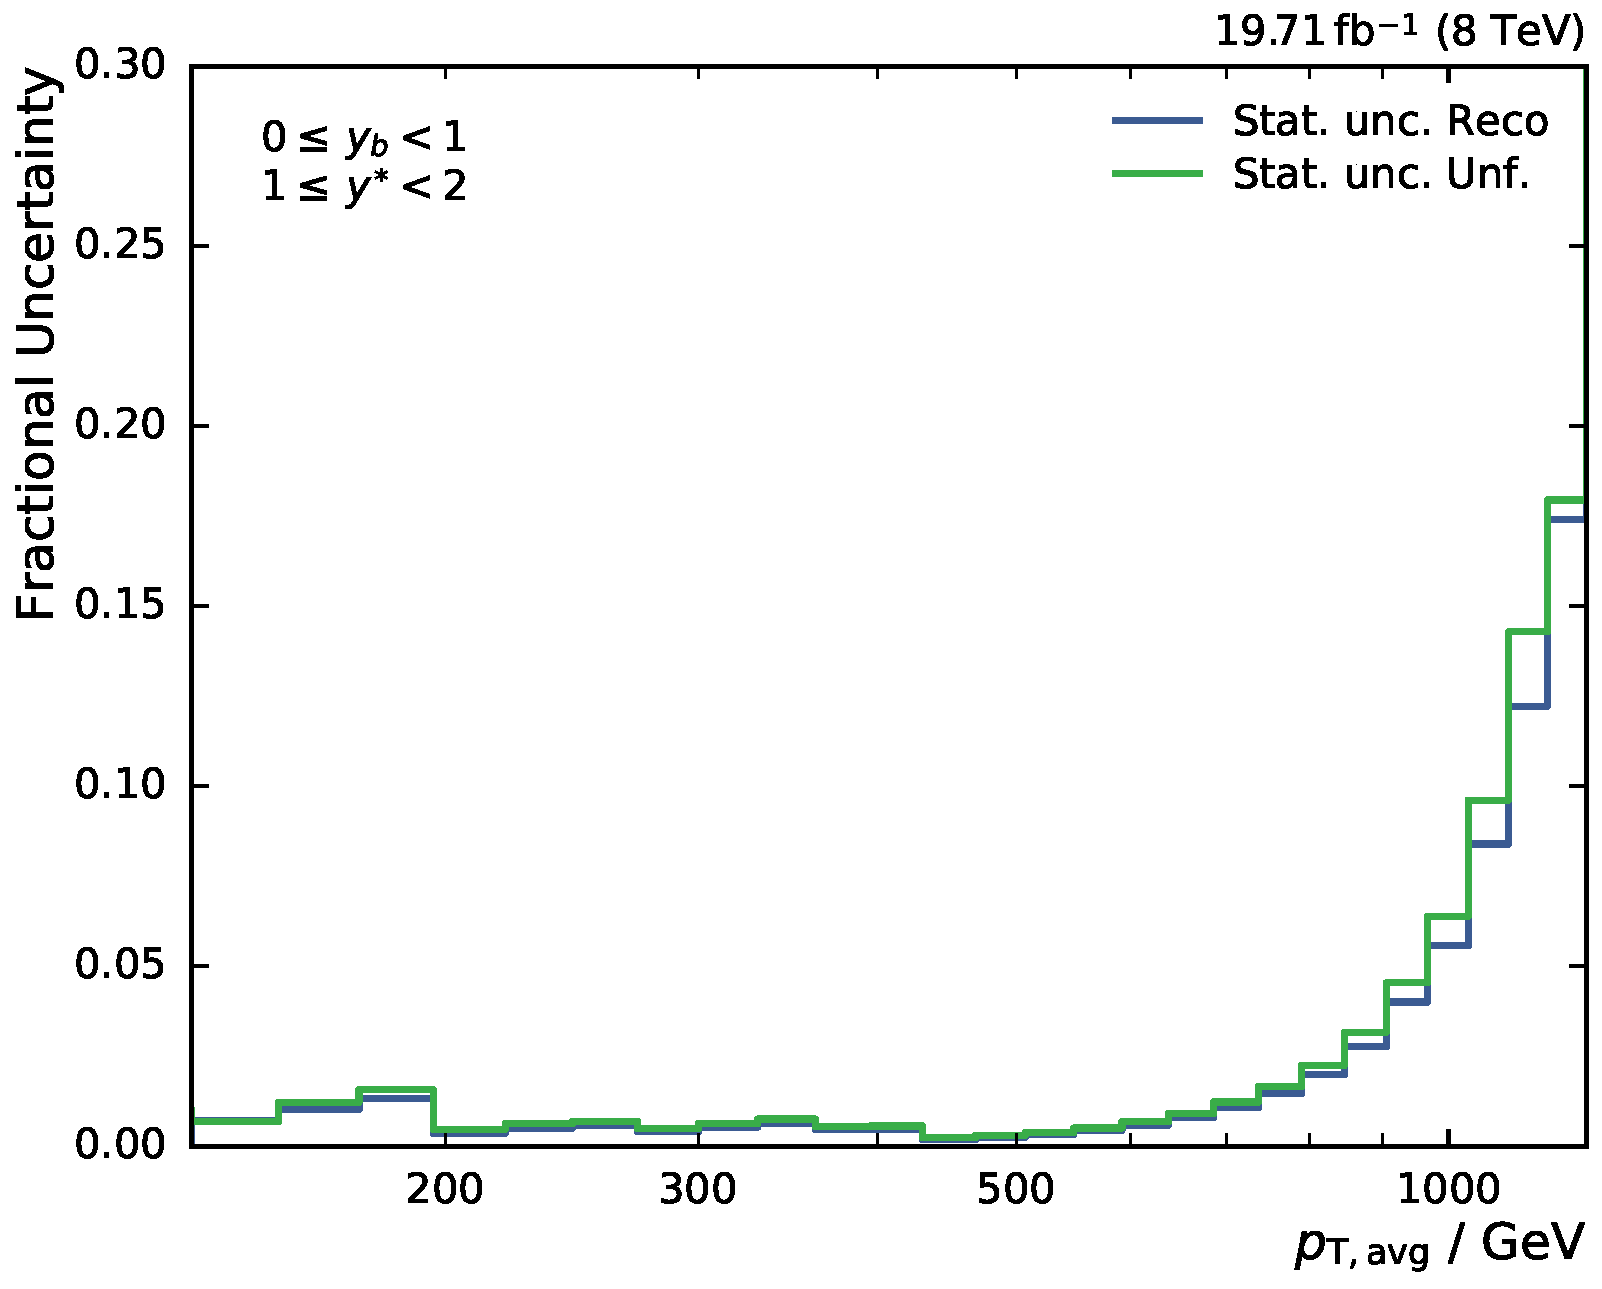
\includegraphics[width=0.45\textwidth]{figures/measurement/statunc_fractional_yb0ys1.pdf}
    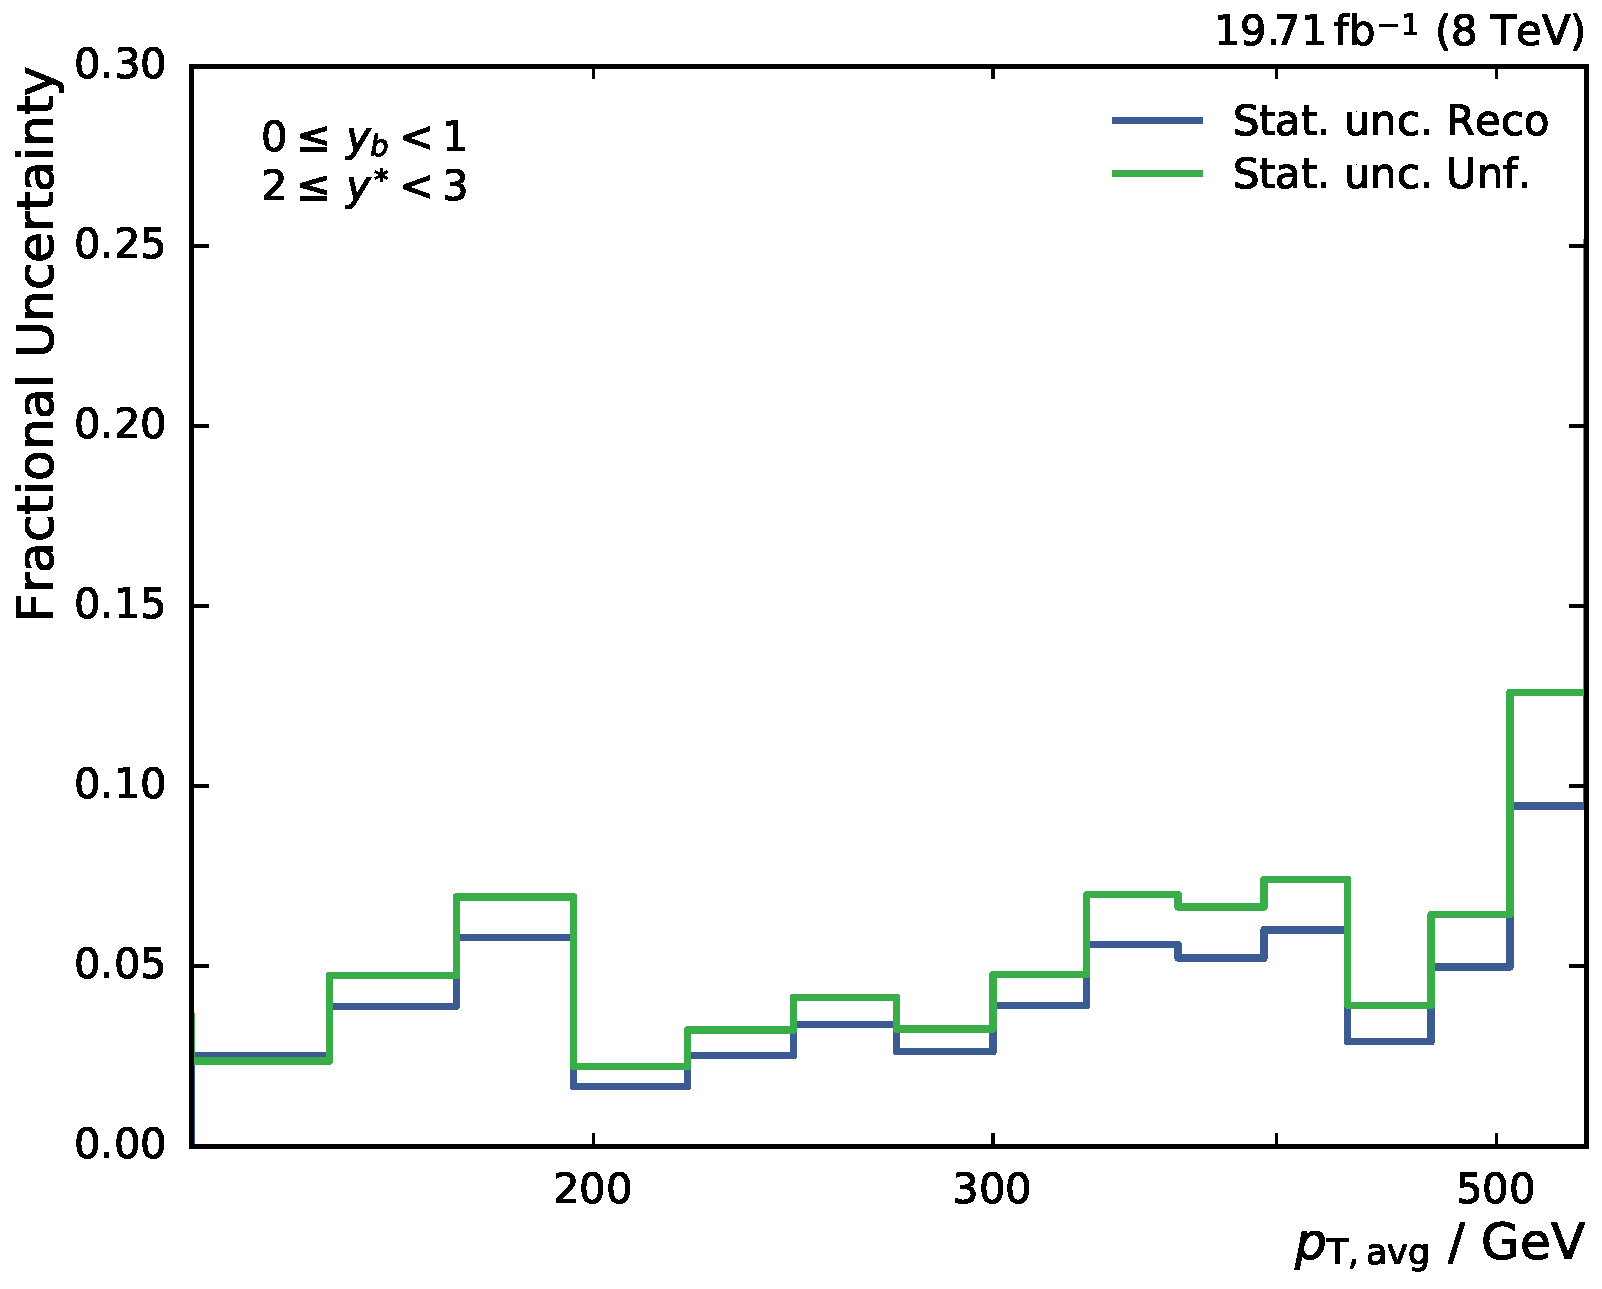
\includegraphics[width=0.45\textwidth]{figures/measurement/statunc_fractional_yb0ys2.pdf}\hfill
    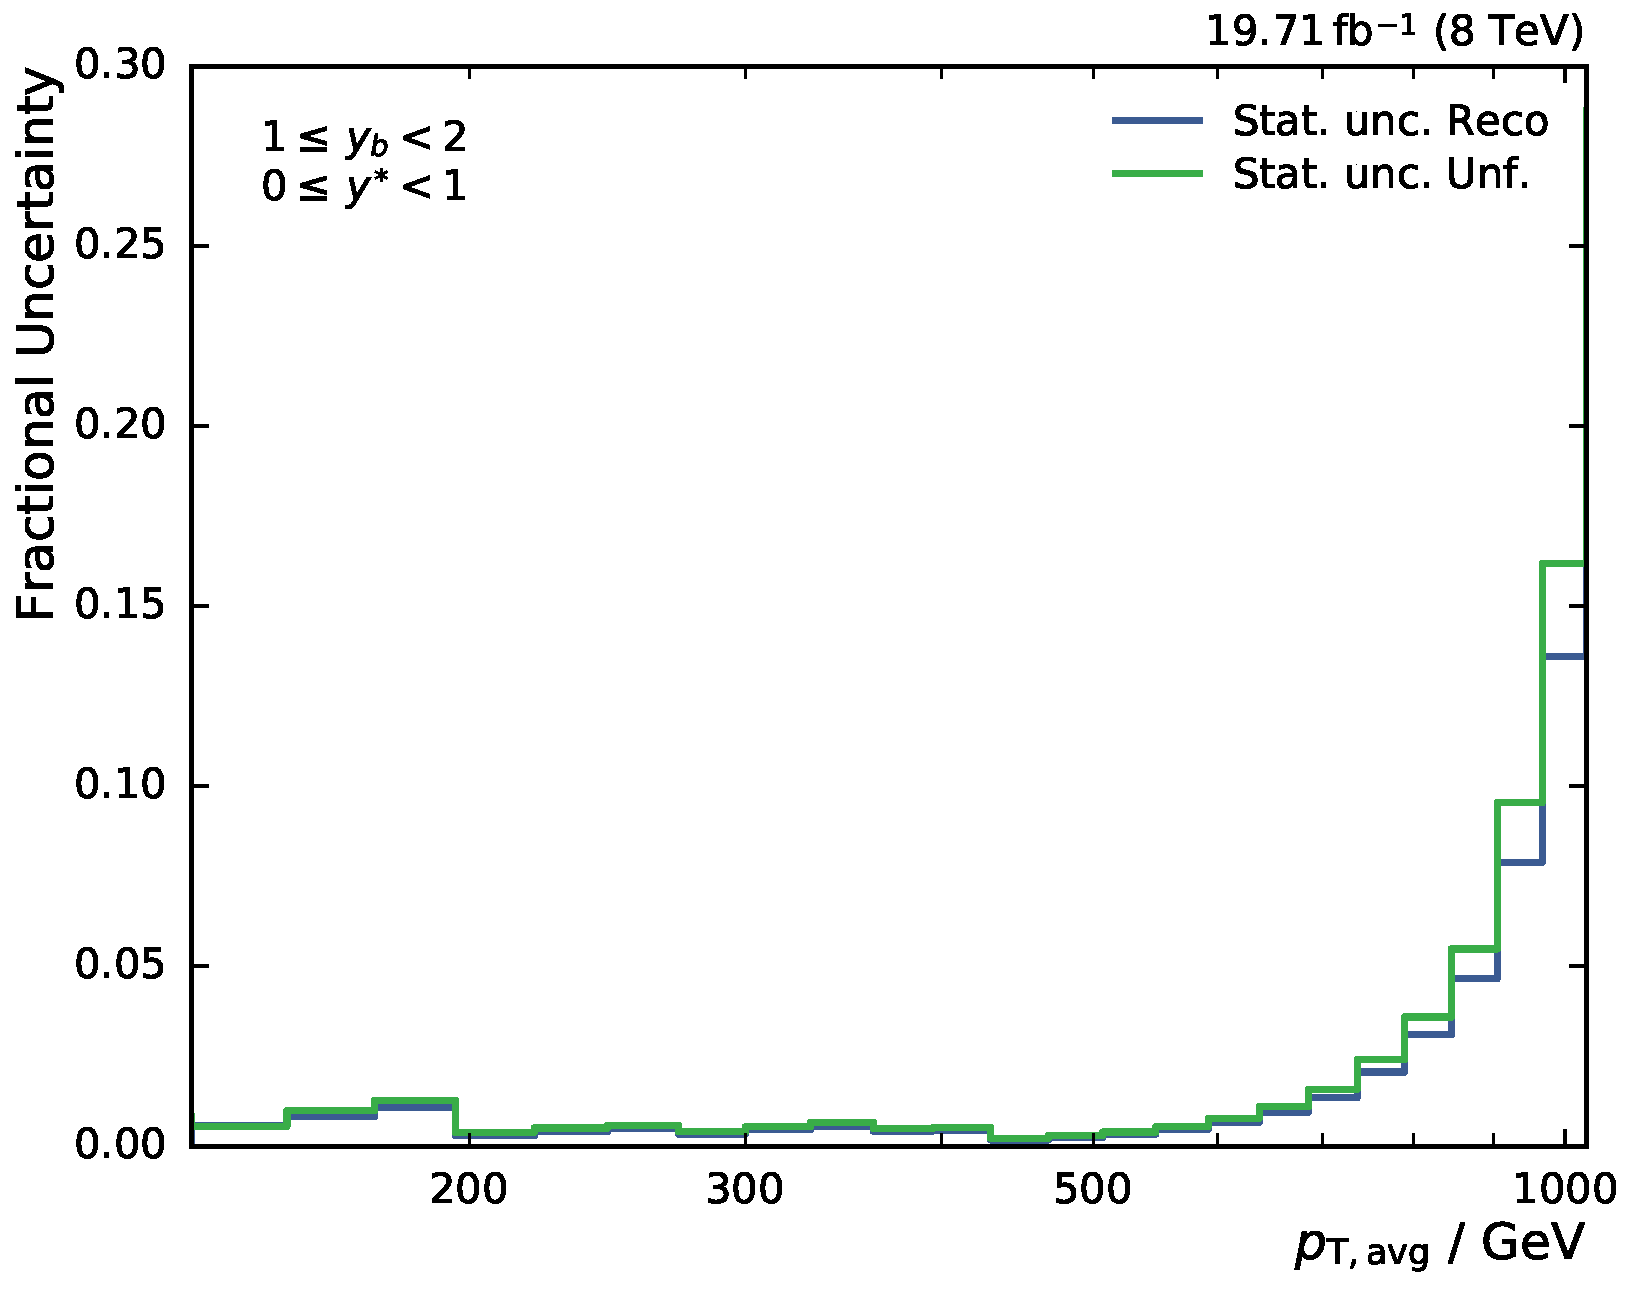
\includegraphics[width=0.45\textwidth]{figures/measurement/statunc_fractional_yb1ys0.pdf}
    \includegraphics[width=0.45\textwidth]{figures/measurement/statunc_fractional_yb1ys1.pdf}\hfill
    \includegraphics[width=0.45\textwidth]{figures/measurement/statunc_fractional_yb2ys0.pdf}
    \caption[Statistical uncertainty of measured and unfolded sprectrum]{The statistical uncertainties of the measured and the unfolded spectrum. Due
    to the unfolding procedure, the uncertainties slightly increase compared to the
    measured spectrum.}
    \label{fig:statunc_relative}
\end{figure}

Futhermore, the unfolding introduces a correlation between bins due to bin
migrations. These correlations are significant for neighbouring bins in \pt and
negligible for far off bins. Figure~\ref{fig:corr_unfolding_nlo} shows the
correlations of the statistical uncertainty after the unfolding.

\begin{figure}[htbp]
    \centering
    \includegraphics[width=0.45\textwidth]{figures/measurement/unf_nlo_corr_yb0ys0.pdf}\hfill
    \includegraphics[width=0.45\textwidth]{figures/measurement/unf_nlo_corr_yb0ys1.pdf}
    \includegraphics[width=0.45\textwidth]{figures/measurement/unf_nlo_corr_yb0ys2.pdf}\hfill
    \includegraphics[width=0.45\textwidth]{figures/measurement/unf_nlo_corr_yb1ys0.pdf}
    \includegraphics[width=0.45\textwidth]{figures/measurement/unf_nlo_corr_yb1ys1.pdf}\hfill
    \includegraphics[width=0.45\textwidth]{figures/measurement/unf_nlo_corr_yb2ys0.pdf}
    \caption[Correlations of statistical uncertainty]{Correlation of the
        statistical uncertainty introduced by the unfolding procedure.
        Neighbouring bins have a significant correlation or anti-correlation
        through bin-by-bin migrations.}
    \label{fig:corr_unfolding_nlo}
\end{figure}

\subsection{Jet Energy Correction Uncertainty}

The dominant part of the experimental uncertainties comes from jet energy
calibration, which correct the measured jet energy for a variety of detector
effects, see Sec.~\ref{sec:jec}. As the corrections are afflicted with multiple
sources of systematic uncertainty, these are propgated individually to the cross section
measurement to conserve all correlations.

The JEC uncertainties are split into 25 mutually independent sources of
uncertainty (JES), in which each source is fully correlated in \pt and $\eta$
and presents a $1\sigma$ shift. As these uncertainties can be asymmetric, the
upwards and downwards variation are treated separately. The sum in quadrature of
all uncertainty sources equals the total uncertainty. Therefore they can be
treated exactly like the PDF eigenvectors sets, which were discussed in
Sec.~\ref{sec:pdf_uncertainties}. The sources of uncertainties are grouped in
four categories which relate to the underlying correction. In the following
list, a short summary of the sources of uncertainty is given. The calibration
procedure and the uncertainties are described in great detail
in~\cite{jec_paper}.

\begin{description}
    \item[Pile-up JES] Differences in the transverse momentum between the true
        offset and the random cone offset observed in simulation. This
        difference is propagated using Z/$\gamma$+jet and dijet balancing
        methods to estimate the residual pileup uncertainty after the
        calibration.
    \item[Relative JES] The relative $\eta$-dependent corrections calibrate
        forward jets using balanced dijet events. The largest contribution to
        the uncertainty arises from jet energy resolution and soft-radiation
        bias corrections. 
    \item[Absolute JES]  The absolute calibration of the jet energy scale relies
        on Z/$\gamma$+jet and multijet events. The uncertainties are related to
        the lepton momentum scale for muon and the single-pion response in the
        HCAL. Observed differences in applied methods, traced back to neutrinos
        and ISR, are also accounted for. 
    \item[Flavor JES] Differences in the flavor response are studied using
        simulation by cross-checking the results with quark- and gluon-tagged
        photon+jet and Z+jet events. The uncertainty is derived based on
        differences observed in the Pythia6 and Herwig++ simulation.
\end{description}

\subsection{Jet Energy Resolution Uncertainty}

The jet energy resolution, as derived in Sec.~\ref{sec:resolution}, influences
the unfolding and consequently introduces a further source of uncertainty on the
unfolded cross section. 

Table~\ref{tab:res_smearing} shows the smearing factors, which were applied on
MC to obtain the actual resolution in data. The official recommendations involve
an uncertainty on this smearing factor to estimate an uncertainty on the
determined resolution, see the varied smearing factors in
Table~\ref{tab:res_smearing}. The resolution determination is repeated with the
up- and downwards variation of the resolution smearing factor $c$ applied. The
unfolding procedure is also reiterated using the variations of the resolution
and the differences of the obtained cross section to the nominal cross section
is accounted for as an additional uncertainty. 

The uncertainty on the cross section is rather small, about 1\% at low rapidity
and increasing to 2\%-3\% at larger rapidities, see
Fig.~\ref{fig:exp_unc_overview}.


\begin{figure}[htbp]
    \centering
    \includegraphics[width=0.45\textwidth]{figures/measurement/exp_unc_overview_yb0ys0.pdf}\hfill
    \includegraphics[width=0.45\textwidth]{figures/measurement/exp_unc_overview_yb0ys1.pdf}
    \includegraphics[width=0.45\textwidth]{figures/measurement/exp_unc_overview_yb0ys2.pdf}\hfill
    \includegraphics[width=0.45\textwidth]{figures/measurement/exp_unc_overview_yb1ys0.pdf}
    \includegraphics[width=0.45\textwidth]{figures/measurement/exp_unc_overview_yb1ys1.pdf}\hfill
    \includegraphics[width=0.45\textwidth]{figures/measurement/exp_unc_overview_yb2ys0.pdf}
    \caption[Overview of experimental uncertainties]{Overview of all
    experimental uncertainties affecting the cross section measurement. The
    errorbars indicate the statistical uncertainty after unfolding. The colored
    lines give the uncertainties resulting of jet energy corrections, jet energy
    resolution, luminosity and residual effects. The total uncertainty is yielded by
    adding in quadrature the individual sources of uncertainty.}
    \label{fig:exp_unc_overview}
\end{figure}

\section{Comparison with NLO Predictions}
\label{sec:nlo_comparisons}

The triple-differential dijet cross section measurement is round off by
comparing the results of the measurement with the NLO cross section calculations
obtained in Sec.~\ref{sec:theory_predictions}. A general comparison is given in
Fig.~\ref{fig:measurement_result} which shows the data overlayed with the NLO
theory prediction obtained with the CT14-NLO PDF set. The measurement and the
prediction agree over eight orders of magnitude in cross section and up to
highest transverse momenta.

\begin{figure}[h!tbp]
    \centering
    \includegraphics[width=0.9\textwidth]{figures/measurement/ptavg_spectrum.pdf}\hfill
    \caption[Spectrum of the Triple-differential Dijet Cross Section]{The
    triple-differential dijet cross section in 6 bins of \ystar and \yboost. The
    data is indicated by different markers for each bin and the theory obtained with CT14-NLO by
    colored lines.}
    \label{fig:measurement_result}
\end{figure}

A detailed comparison revealing plenty of further effects is possible py
calculating the ratio of the data to the theory calculation.
Figures~\ref{fig:ratio_ct14_nlo}---\ref{fig:ratio_nnpdf30_nlo} show the ratio to
data of the theory calculation with the CT14 PDF set and the NNPDF 3.0 PDF set,
respectively. To emphasize effects due to the different PDFs, the ratio figures
include also the predictions obtained with the MMHT 2014 PDF set and the ABM11
PDF set. The predictions with the different PDF sets agree with each other apart
from ABM 11. The differences caused by ABM 11 are well known and seen in a
multitude of further jet measurements and are due to a soft gluon PDF
accompanied by a low value of \asmz in this PDF set. 

A further effect in which all theory predictions differ from the data, is
prominently visible in the central region at large transverse momenta. The
theory predictions underestimates the data by up to 20\%. This effect has been
observed earlier and can be attributed to the missing electroweak corrections
which are positive and sizeable at low rapidity and high transverse momenta.
Theory colleagues are currently working on providing the electroweak corrections
specifically for this measurement, but they were not available in
time\todo{check for ewk}.

\begin{figure}[htbp]
    \centering
    \includegraphics[width=0.45\textwidth]{figures/measurement/ratio_to_CT14nlo+np_totcomp_yb0ys0.pdf}\hfill
    \includegraphics[width=0.45\textwidth]{figures/measurement/ratio_to_CT14nlo+np_totcomp_yb0ys1.pdf}
    \includegraphics[width=0.45\textwidth]{figures/measurement/ratio_to_CT14nlo+np_totcomp_yb0ys2.pdf}\hfill
    \includegraphics[width=0.45\textwidth]{figures/measurement/ratio_to_CT14nlo+np_totcomp_yb1ys0.pdf}
    \includegraphics[width=0.45\textwidth]{figures/measurement/ratio_to_CT14nlo+np_totcomp_yb1ys1.pdf}\hfill
    \includegraphics[width=0.45\textwidth]{figures/measurement/ratio_to_CT14nlo+np_totcomp_yb2ys0.pdf}
    \caption[Ratio of the cross section to CT14 NLO]{
    Ratio of the triple-differential dijet cross sections to the theoretical
    prediction using the central value of the CT14 NLO PDF set for each bin in \ystar
    and \yboost respectively. The datapoints including statistical uncertainty are
    indicated by markers, the total experimental uncertainty is represented by the
    hatched red band. The solid blue band indicates the PDF uncertainty and the
    continous colored lines the predictions of the cross sections calculated with
    other PDF sets. }
    \label{fig:ratio_ct14_nlo}
\end{figure}

\begin{figure}[htbp]
    \centering
    \includegraphics[width=0.45\textwidth]{figures/measurement/ratio_to_NNPDF30+np_totcomp_yb0ys0.pdf}\hfill
    \includegraphics[width=0.45\textwidth]{figures/measurement/ratio_to_NNPDF30+np_totcomp_yb0ys1.pdf}
    \includegraphics[width=0.45\textwidth]{figures/measurement/ratio_to_NNPDF30+np_totcomp_yb0ys2.pdf}\hfill
    \includegraphics[width=0.45\textwidth]{figures/measurement/ratio_to_NNPDF30+np_totcomp_yb1ys0.pdf}
    \includegraphics[width=0.45\textwidth]{figures/measurement/ratio_to_NNPDF30+np_totcomp_yb1ys1.pdf}\hfill
    \includegraphics[width=0.45\textwidth]{figures/measurement/ratio_to_NNPDF30+np_totcomp_yb2ys0.pdf}
    \caption[Ratio of the cross section to NNPDF 3.0 NLO]{
    Ratio of the triple-differential dijet cross sections to the theoretical
    prediction using the central value of the NNPDF 3.0 NLO PDF set for each bin in \ystar
    and \yboost respectively. The datapoints including statistical uncertainty are
    indicated by markers, the total experimental uncertainty is represented by the
    hatched red band. The solid blue band indicates the PDF uncertainty and the
    continous colored lines the predictions of the cross sections calculated with
    other PDF sets. }

    \label{fig:ratio_nnpdf30_nlo}
\end{figure}

Especially phase space regions, in which the data discriminates between the
predictions of different PDF sets, are interesting input for PDF studies. As
discussed in Sec.~\ref{sec:crosssection_definition}, the bins involving boosted
same-side dijet events, in which the fractional proton momenta $x_1$ and $x_2$
are very different, are predestined for PDF studies. The predictions of the
different PDF sets, especially the NNPDF PDF set, yield different results and
are afflicted with a large PDF uncertainty. Moreover, none of the investigated
PDF sets yields a good description of the data in this phase space region, see
bottom right plot in Fig.~\ref{fig:ratio_ct14_nlo}.



